%%%%%%%%%%%%%%%%%%%%%%%%%%%%%%%%%%%%%%%%%%%%%%%%%%%%%%%%%%%%%%%%%%%%%%%%%%%%%%%%%%%%%%%%%
%									TESIS DE DOCTORADO
%								CHRISTIAN FABIAN GARCIA ROMERO
%							   UNIVERSIDAD NACIONAL DE COLOMBIA
%
%%%%%%%%%%%%%%%%%%%%%%%%%%%%%%%%%%%%%%%%%%%%%%%%%%%%%%%%%%%%%%%%%%%%%%%%%%%%%%%%%%%%%%%%%


%%%%%%%%%%%%%%%%%%%%%%%%%%%%%%%%%%%%%%%%%%%%%%%%%%%%%%%%%%%%%%%%%%%%%%%%%%%%%%%%%%%%%%%%%

% TERCER CAPITULO: PROCESOS DE MODELAMIENTO EN ACOPLAMIENTO GEOMECÁNICO

%%%%%%%%%%%%%%%%%%%%%%%%%%%%%%%%%%%%%%%%%%%%%%%%%%%%%%%%%%%%%%%%%%%%%%%%%%%%%%%%%%%%%%%%%

%----------------------------------------------------------------------------------------
% TITULO DEL CAPITULO 3
\chapter{Modelo Geomecánico Totalmente Acoplado}~\hypertarget{chapter_03}{}
\label{ch:chapter_03}

Para la creación del nuevo marco metodológico se parte de un modelo matemático general, el cual se mejora paulatinamente hasta encontrar una serie de modelos mejorados. En este capitulo se describe ese modelo el cual se conoce en la literatura como un \textit{Modelo Geomecánico Totalmente Acoplado-(MGTA)}. Como se explicó en la ~\MYhref[blue]{sec:sec22}{\textit{Sección 2.2: Metodologías de Acoplamiento}}, este modelo se caracteriza por solucionar de manera simultanea las (\textit{EDP}) que representan la física del problema.\bigskip

Para obtener el modelo (\textit{MGTA}) se utiliza la metodología para el modelamiento en medios porosos presentada en la ~\MYhref[blue]{sec:sec23}{\textit{Sección 2.3}}. Según esa metodología se inicia planteando el modelo conceptual, que de manera general establece las bases y simplificaciones para el modelamiento de problemas de flujo. Después se obtiene el modelo matemático, que plantea la formulación de ecuaciones que rigen el problema físico. En un tercer paso, se utiliza el método de los elementos finitos (\textit{MEF}) para hallar el modelo numérico. Finalmente se crea código Python a partir del modelo numérico y se obtiene el modelo computacional del problema. \bigskip


Al final de este capítulo se evidencia una serie de simulaciones numéricas de tres tipos de problemas comunes de acoplamiento geomecánico, todos en presencia de un medio poroso elástico e isotópico: (1) Consolidación Unidimensional; (2) Consolidación bidimensional; (3) Problema “\textit{Five-Spot}” en presencia de flujo bifásico~\footnote{El problema “\textit{Five-Spot}” es común en la ingeniería de reservorios, y se caracteriza por la inyección de un fluido (e.g. gas o agua), en el medio poroso a través de 4 pozos de inyección, y la producción de un segundo tipo de fluido (e.g petroleo) por un solo pozo de producción. Ver \href{https://www.spe.org/web/csp/datasets/set02.htm}{SPE10 Benchmark} para mayor información.}.\bigskip

Con estas simulaciones se verificó que todos estos modelos fueron determinados de manera correcta y son representativos de la física del problema. En capítulos posteriores se toma como base este modelo totalmente acoplado para hacer mejoras en la precisión, exactitud de los resultados y en los tiempos de simulación.
%----------------------------------------------------------------------------------------


%----------------------------------------------------------------------------------------
% TITULO DE LA SECCIÓN 3.1
\section{Modelo Conceptual}~\hypertarget{sec:sec310}{}
\label{sec:sec310}

El modelo conceptual es la colección de supuestos y descripciones de procesos físicos que representan el comportamiento físico de la realidad de interés. A partir de este modelo se pueden construir el modelo matemático y los experimentos de verificación. Un requisito fundamental para la construcción del modelo conceptual es partir de un proceso físico real. El acoplamiento geomecánico se pueden aplicar a varias situaciones reales donde se involucre geomateriales de tipo poroso. Del análisis de la literatura se puede encontrar diversas aplicaciones reales de este tipo de modelo:


\begin{itemize}
    \item Asentamiento y consolidación
    \item Estabilidad de taludes
    \item Manejo de acuíferos
    \item Excavaciones de minas y túneles
    \item Subsidencia y compactaciones de reservorios
    \item Desenvolvimiento de campos de petróleo y gas
    \item Estabilidad de pozos de agua, petróleo y gas
    \item Producción de arena en pozos 
    \item Secuestro de $CO_{2}$
    \item Disposición de residuos peligrosos
    \item Fracturamiento hidráulico

\end{itemize}

Sin importar cual sea la aplicación en concreto que se desee predecir, el modelo conceptual debe tener en cuenta dos tipos de parámetros: (1) Los referentes a las propiedades mecánicas de los medios porosos involucrados; (2) Las características termo-hidráulicas de los materiales presentes; (3) La geometría del dominio y del contorno del problema; (4) Características de la ejecución física del proyecto. Para la determinación de los modelos conceptuales que hacen parte de esta investigación se deben responder tres preguntas:

\begin{enumerate}
    \item  ¿Qué conocemos del problema?
    \item  ¿Qué estamos buscando predecir?
    \item  ¿Cuál es el comportamiento mecánico de los materiales?
\end{enumerate}


%----------------------------------------------------------------------------------------
\subsection{¿Qué conocemos del problema?}~\hypertarget{sec:sec311}{}
\label{sec:sec311}

En cualquier aplicación de acoplamiento geomecánico se tienen una seria de datos que se conocen y otros que son inciertos. Otro tipos de datos son iniciales, pero cambian con el desarrollo del proyecto. Estas características se pueden unir en un solo esquema, que se conoce en modelamiento como un \textit{“Problema de valor inicial y de contorno”– (PVIC)}. Establecer con detalle este tipo de problema, responderá la pregunta y determinará con claridad que sabemos y que no sabemos del problema.\bigskip 

Existen varios tipos de problemas acoplados, que envuelven la determinación de dos o más incógnitas. Cada uno de estos tipos de acoplamiento representa una clase diferente de problema (\textit{PVIC}), como se muestra en la \textbf{Tabla} \textbf{\ref{tab:tabla31}}. Por lo tanto, al inicio del proyecto es fundamental decidir qué tipo de problema acoplado estamos abordando y así establecer lo que conocemos. Para esta investigación solo se afrontarán problemas de dos tipos, es decir, \textit{“Problemas de valor inicial y de contorno flujo-geomecánico”– (PVIC-HG)}  y \textit{“Problemas de valor inicial y de contorno termo-flujo-geomecánico”– (PVIC-THG)}.\bigskip


%#######################################################################################
% TABLA 3.1
\begin{table}[!ht]
\centering
\caption{Tipos de problemas (\textit{PVIC}) en acoplamiento geomecánico}
\vspace*{4mm}
\label{tab:tabla31}
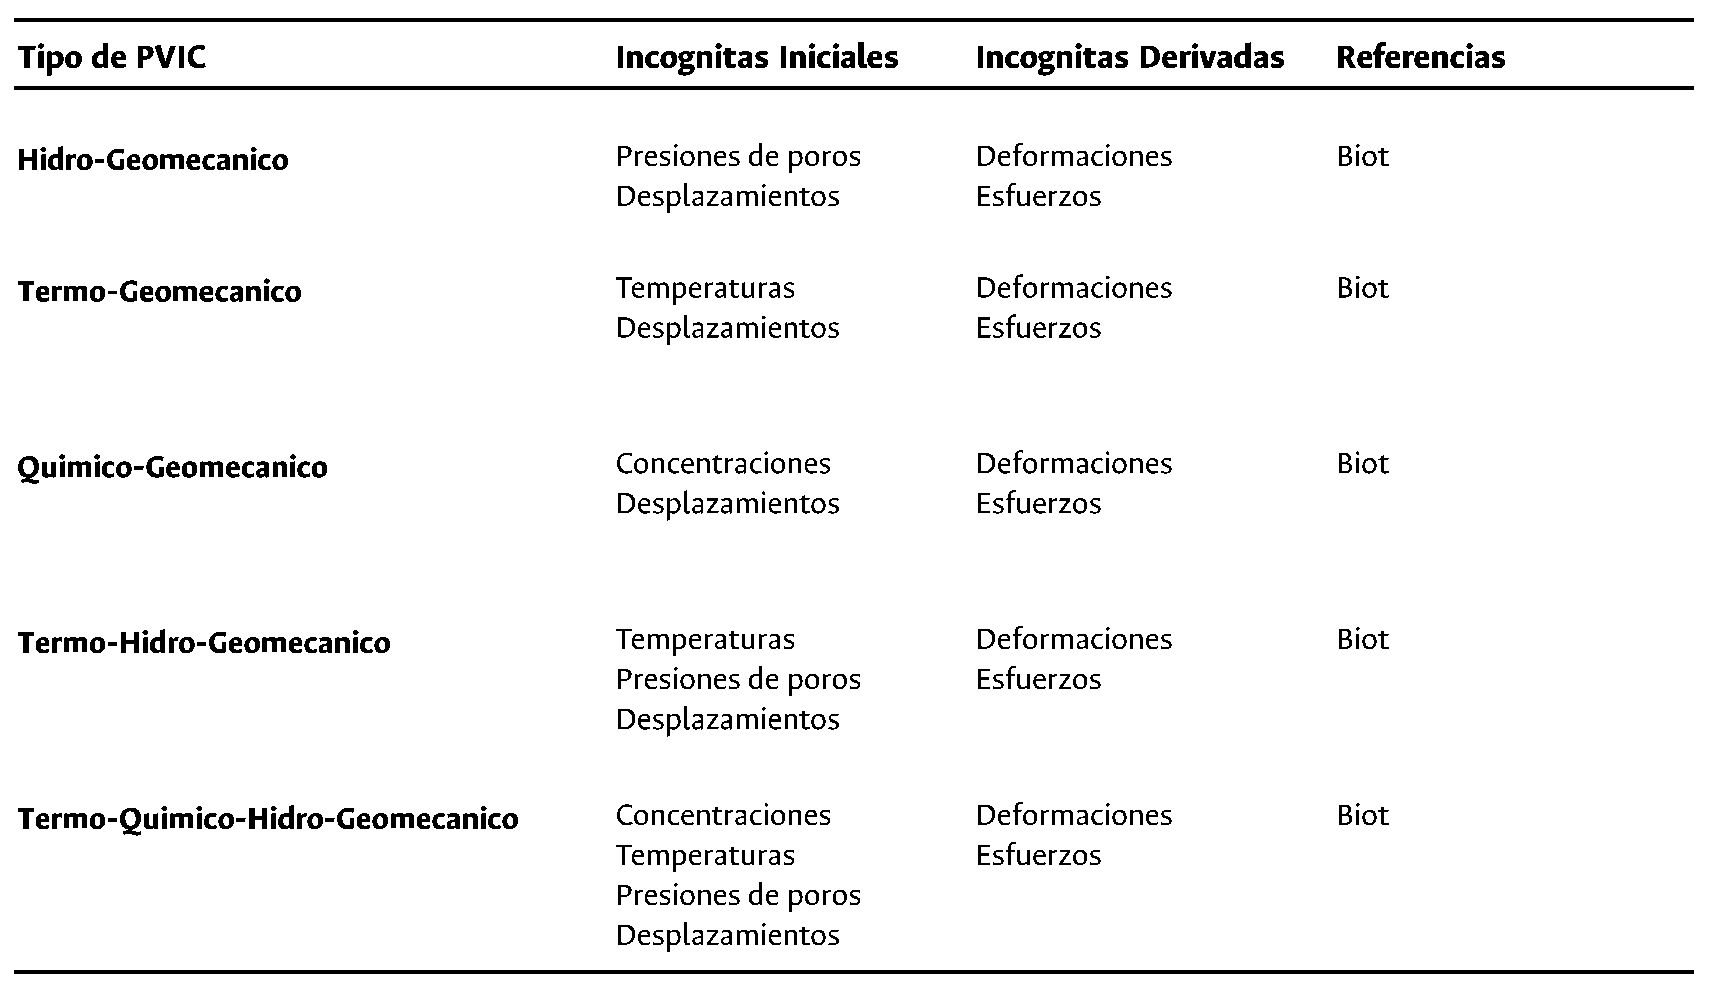
\includegraphics[width=1.0\textwidth]{Tablas/Kap_03/Tipos_PVIC.png}
\end{table}
%########################################################################################

Ya teniendo claro este concepto, podemos establecer las características del modelo conceptual que se debe determinar para poder seguir desarrollando el modelo acoplado. Esas características del modelo conceptual son:

\begin{itemize}
    \item \textbf{Geometría del problema}: Establecer un dominio y sus dimensiones
    \item \textbf{Materiales}: Medios porosos y fluidos presentes con sus características físicas
    \item \textbf{Condiciones iniciales}: Valores de las incógnitas al inicio del proyecto
    \item \textbf{Condiciones de contorno}: Restricciones y grados de libertad del problema
\end{itemize}
\bigskip

%----------------------------------------------------------------------------------------
\subsection{¿Qué estamos buscando predecir?}~\hypertarget{sec:sec312}{}
\label{sec:sec312}

La respuesta a esta pregunta está en la \textbf{Tabla} \textbf{\ref{tab:tabla31}}, en la columna de incógnitas. Estas incógnitas iniciales se pueden determinar directamente del modelo matemático, pero existen "\textit{incógnitas derivadas}", que son de igual o mayor importancia, pero se determinan después de resolver el sistema inicial. Específicamente para acoplamiento un problema (\textit{PVIC-FG}) se pueden determinar estas "\textit{incógnitas derivadas}":

\begin{itemize}
    \item Esfuerzos y deformaciones
    \item Producción de fluidos en pozos
    \item Gradientes hidráulicos, Entre otros.
\end{itemize}

Ya es cuestión tanto del problema como del modelador establecer rutinas de cálculo para la determinación de estas magnitudes. Estas decisiones se deben llevar a cabo en el modelo conceptual para que los modelos posteriores tengan en cuentas estas necesidades y se establezcan las ecuaciones y el código necesario.\bigskip

%----------------------------------------------------------------------------------------
\subsection{¿Cuál es el comportamiento mecánico de los materiales?}~\hypertarget{sec:sec313}{}
\label{sec:sec313}

Por último, pero de gran importancia es establecer los comportamientos mecánicos de los materiales que hacen parte del dominio. Estas características mecánicas se pueden establecer en relaciones constitutivas y características físicas. Lo más común es establecer:

\begin{itemize}
    \item Modelos constitutivos de suelos y rocas
    \item Relaciones constitutivas hidráulicas (e.g. curvas de retención)
    \item Compresibilidad de los fluidos
    \item Cuáles son las fases de los fluidos (i.e. gaseoso, liquido)
    \item Isotropía o anisotropía
    \item Permeabilidades y porosidades de los suelos y rocas, entre otros.
\end{itemize}
%\newpage



%----------------------------------------------------------------------------------------
% TITULO DE LA SECCIÓN 3.2
\section{Modelo Matemático}~\hypertarget{sec:sec320}{}
\label{sec:sec320}

La modelación matemática tiene como objetivo describir los diferentes aspectos del mundo real, su interacción y su dinámica a través de ecuaciones matemáticas. Constituye uno de los pilares de la ciencia y la ingeniería, logrando el desarrollo de dos disciplinas más tradicionales, como lo son el análisis teórico y la experimentación  \cite{Quarteroni2009MathematicalEngineering}.\bigskip

En reservorios de petroleo y gas existen diversos fenómenos físicos que se pueden modelar a través de (\textit{EDP}). Cuando se comienza la producción de hidrocarburos en estos reservorios a través de pozos de producción, ocurren simultáneamente fenómenos de flujo, geomecánicos y termodinámicos. Estos tipos de proyectos energéticos, se pueden modelar con la ayuda de modelos geomecánicos acoplados como los expuestos en la \textbf{Tabla} \textbf{\ref{tab:tabla31}}.\bigskip

Es común en la literatura de ingeniería de reservorios modelar la producción de hidrocarburos a través del \textit{Modelo Black-Oil}, el cual es un modelo de comportamiento multifásico que es estándar en la industria del petroleo. Este modelo es capaz de predecir la compresibilidad y los efectos de transferencia de masa entre fases (i.e. gas, petroleo, agua). La importancia del \textit{Modelo Black-Oil} para los estudios de ingeniería de reservorios lo convierte en un modelo importante para investigadores interesados en desarrollar nuevos métodos para la solución de (\textit{EDP}) de flujo multifásico en cualquier medio poroso\cite{Huan1986TheReservoir}.\bigskip

El \textit{Modelo Black-Oil} es un modelo de flujo trifásico donde se puede modelar el flujo de tres fases: (1) Agua; (2) Petroleo; (3) Gas. La fase gaseosa puede estar libre y/o disuelta en el petroleo. En este modelo se asume que el petroleo y el gas son materiales homogéneos, pero estos hidrocarburos están constituidos por muchos componentes orgánicos, pero se simplifica el comportamiento como si fueran materiales homogéneos, como lo es el agua.\bigskip

En esta sección se plantea un modelo general a partir del \textit{Modelo Black-Oil}, adicionando las características mecánicas de un modelo geomecánico no-isotérmico. Con esto se crea un modelo termo-flujo-geomecánico cuyas características principales son:

\begin{itemize}
    \item Modelo totalmente acoplado en 3-Dimensiones
    \item Flujo trifásico compresible (i.e. gas, petroleo, agua)
    \item Anisotropía (Referente a la permeabilidad del medio poroso)
    \item Relación constitutiva poro-elástica (Biot \cite{Biot1941GeneralConsolidation})
    \item Porosidad dependiente del cambio de esfuerzos
\end{itemize}

A partir de este modelo se pueden obtener otro tipo de modelos que pueden ser aplicados a problemas bifásicos en presencia tanto de suelos como de rocas. Como se puede ver en la Figura 3.1, a partir de este modelo general, que denominaremos "Modelo totalmente acoplado termo-hidro-geomecánico - (MTA-THG)", se pueden obtener los otros modelos aplicando las simplificaciones correspondientes.\bigskip

%////////////////////////////////////////////////////////////////////////////////////////
% FIGURA 3.1
\begin{figure}[!ht]
\centering
\begin{subfigure}[b]{.45\textwidth}
        \centering
        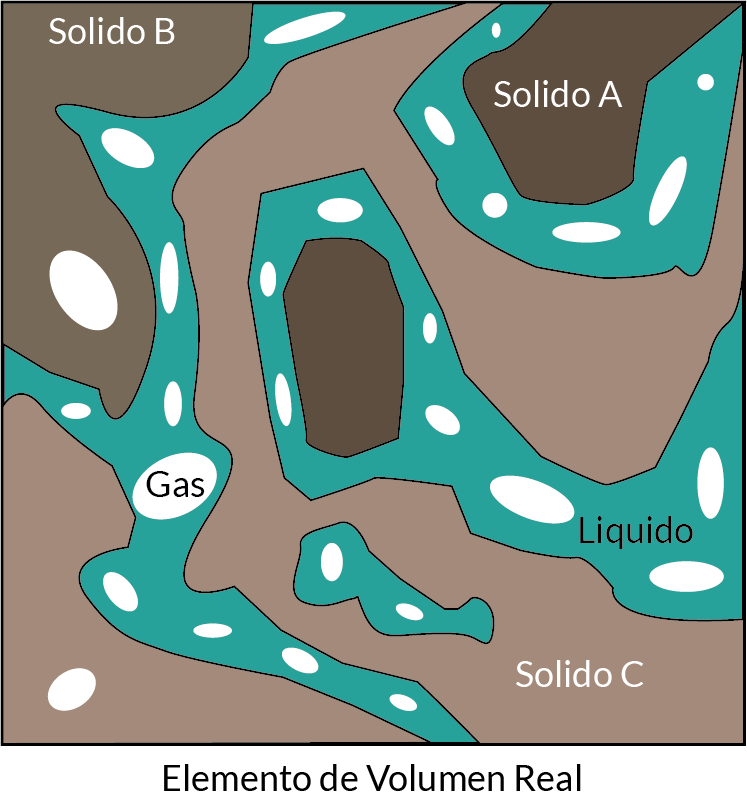
\includegraphics[width=6.5cm]{Imagenes/Kap_03/Real.png}
        \caption{}
        \label{fig:fig31a}
\end{subfigure}
\hfill
\begin{subfigure}[b]{.45\textwidth}
        \centering
        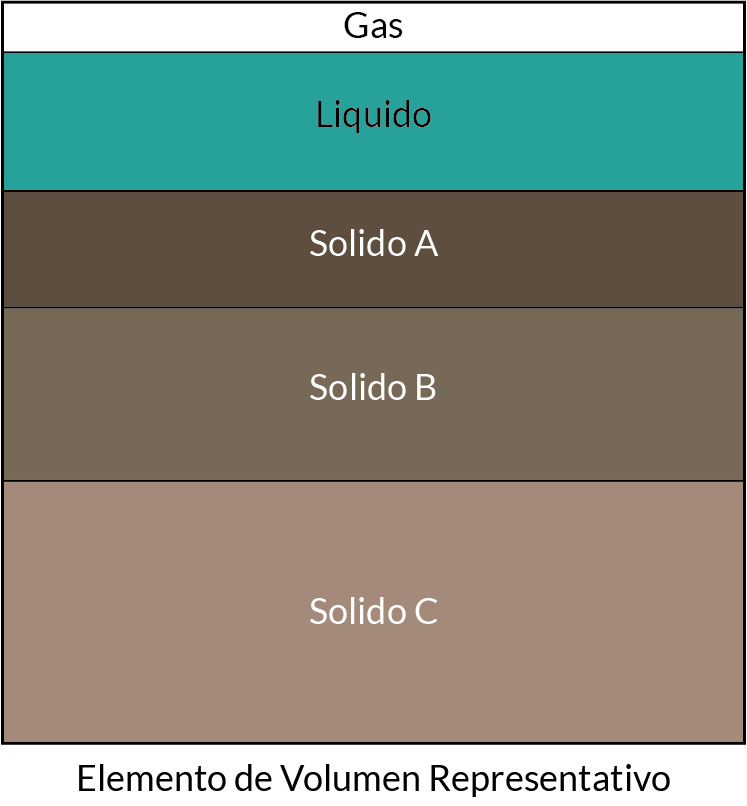
\includegraphics[width=6.5cm]{Imagenes/Kap_03/REV.png}
        \caption{}
        \label{fig:fig31b}
\end{subfigure}
\captionsetup{format=plain}
\caption[Elemento de Volumen Representativo de Medio Poroso]{Elemento de Volumen Representativo de Medio Poroso. (\subref{fig:fig31a}) Elemento de volumen Real; (\subref{fig:fig31b}) Elemento de volumen representativo.} 
%\vspace*{1cm}
\label{fig:fig31}
\end{figure}
%\bigskip
%////////////////////////////////////////////////////////////////////////////////////////


En estado natural un medio poroso de origen geológico, como lo son los suelos y las rocas, está constituido por tres fases como se puede ver en la \textbf{Figura} \ref{fig:fig32}: (1) Fase Solida: Minerales y/o materia orgánica; (2) Fase Liquida: Agua y/o Petróleo; (3) Fase Gaseosa: Aire o Gas Natural.\bigskip

Las características del modelo geomecánico y el modelo de flujo son determinadas por esta característica del medio poroso. El flujo de fluidos en un medio poroso puede ser monofásico cuando fluye un solo tipo de fluido, ya sea agua, petróleo o cualquier tipo de gas. Se dice que el flujo es bifásico si fluyen dos tipos de fluidos, como es el caso de los suelos residuales. Y el flujo trifásico se caracteriza porque fluyen tres tipos de fluidos como es el caso de muchos reservorios de petroleo, ya que fluye agua, gas y petroleo.\bigskip

% %////////////////////////////////////////////////////////////////////////////////////////
% % FIGURA 3.2
% \begin{figure}[!ht]
% \centering
% \begin{subfigure}[b]{.45\textwidth}
%         \centering
%         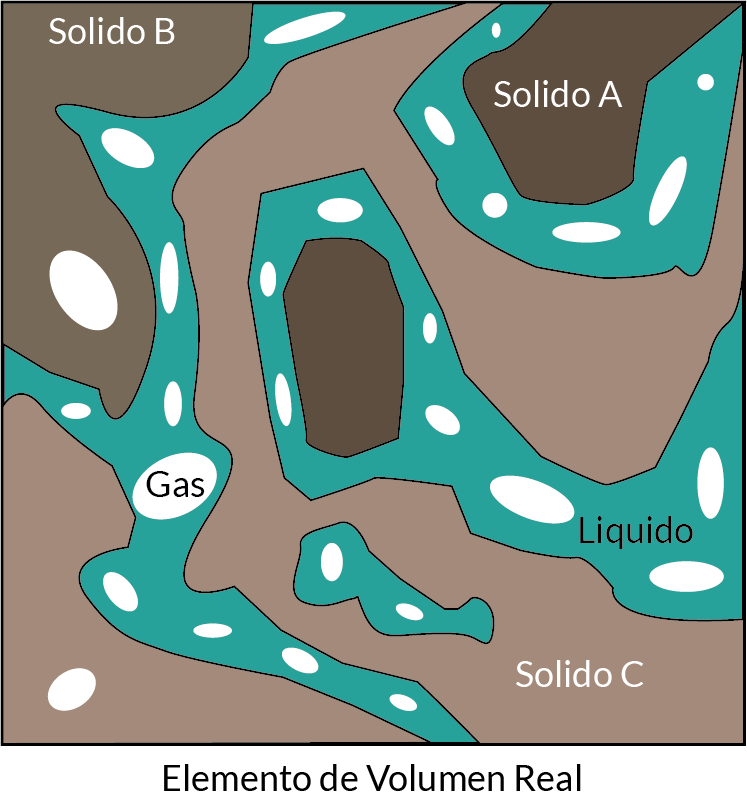
\includegraphics[width=6.5cm]{Imagenes/Kap_03/Real.png}
%         \caption{}
%         \label{fig:fig32a}
% \end{subfigure}
% \hfill
% \begin{subfigure}[b]{.45\textwidth}
%         \centering
%         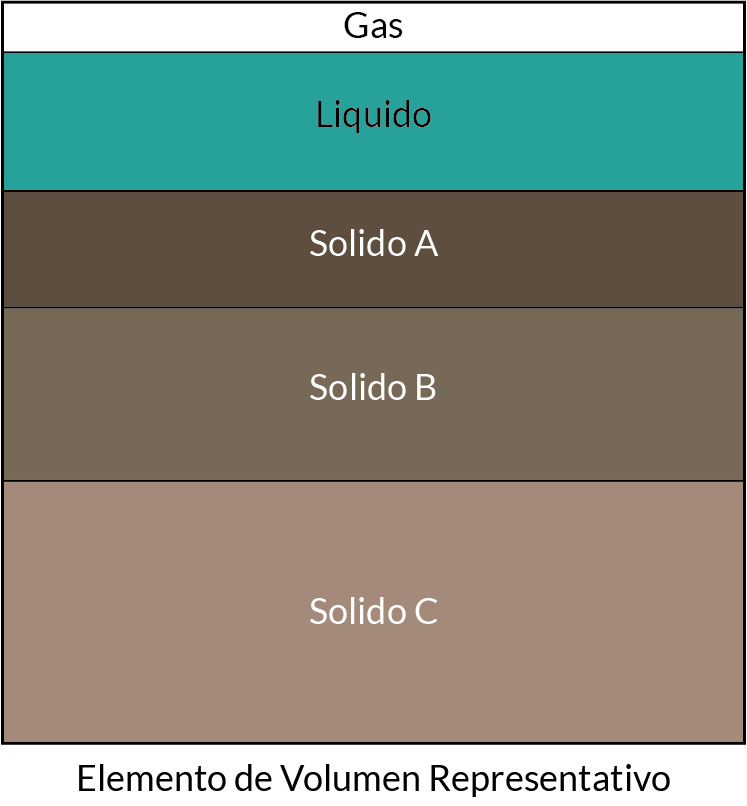
\includegraphics[width=6.5cm]{Imagenes/Kap_03/REV.png}
%         \caption{}
%         \label{fig:fig32b}
% \end{subfigure}
% \captionsetup{format=plain}
% \caption[Elemento de Volumen Representativo de Medio Poroso]{Elemento de Volumen Representativo de Medio Poroso. (\subref{fig:fig31a}) Elemento de volumen Real; (\subref{fig:fig31b}) Elemento de volumen representativo.} 
% %\vspace*{1cm}
% \label{fig:fig32}
% \end{figure}
% %\bigskip
% %////////////////////////////////////////////////////////////////////////////////////////

\bigskip
Todo el desarrollo matemático que se hace de aquí en adelante tiene las siguientes convenciones: (1) Todos los vectores se representan en negrita y con el símbolo $\mathbf{\{\bullet\}}$; (2) Todas las matrices se representan en negrita con el símbolo $\mathbf{\left[\bullet\right]}$; (3) Todos los vectores a menos que se diga lo contrario son vectores columna; (4) El superíndice ($T$) significa el traspuesto de un vector, matriz u operador diferencial; (5) Los valores escalares están representados en texto normal (i.e. sin negrita o cursiva).\newpage


%........................................................................................
% TITULO DE LA SUBSECCIÓN 3.2.1
\subsection{Modelo Geomecánico (\textit{MTA-THG})}~\hypertarget{sec:sec321}{}
\label{sec:sec321}

El comportamiento mecánico de un medio poroso está determinado por su modelo geomecánico o también llamado modelo esfuerzo-deformación. Este modelo permite determinar: (1) Deformaciones; (2) Esfuerzos; (3) Desplazamientos. El modelo geomecánico de un medio poroso se rige por las mismas ecuaciones que definen los medios continuos, como lo son las ecuaciones de equilibrio, compatibilidad de deformaciones y relaciones constitutivas. Cuando se juntan estas tres ecuaciones se define un sistema de (\textit{EDP}) que en esencia es el modelo matemático geomecánico no-acoplado.\bigskip


\textbf{A. Ecuación de Equilibrio}
\\
La ecuación que gobierna la deformación del material sólido se llama ecuación de equilibrio \cite{Shabana2018ComputationalMechanics}. Esta se define en 3-Dimensiones como:

%----------------------------------------------------------------------------------------
% ECUACIÓN 3.1
\begin{ceqn} 
\begin{subequations} \label{eq:equ31} 
\begin{gather}
\frac{\partial\sigma_{xx}}{\partial x} + \frac{\partial\tau_{xy}}{\partial y} + \frac{\partial\tau_{xz}}{\partial z} + b_x = 0 \label{eq:equ31a} \\[5pt]
\frac{\partial\sigma_{yy}}{\partial y} + \frac{\partial\tau_{xy}}{\partial x} + \frac{\partial\tau_{yz}}{\partial z} + b_y = 0 \label{eq:equ31b}\\[5pt]
\frac{\partial\sigma_{zz}}{\partial z} + \frac{\partial\tau_{xz}}{\partial x} + \frac{\partial\tau_{yz}}{\partial y}+ b_z = 0 \label{eq:equ31c}
\end{gather}  
\end{subequations} 
\end{ceqn}
%----------------------------------------------------------------------------------------
donde ($\sigma$) es el esfuerzo normal, ($\tau$) es el esfuerzo cortante, ($b$) las fuerzas de cuerpo. De la ecuación anterior se puede definir:
%----------------------------------------------------------------------------------------
% ECUACIÓN 3.2
\begin{ceqn} 
\begin{subequations} \label{eq:equ32} 
\begin{gather}
[\mathbf{\sigma}] = 
       \begin{bmatrix}
       \sigma_{xx} &  \tau_{xy}   &  \tau_{xz}    \\[0.3em]
       \tau_{xy}   &  \sigma_{yy} &  \tau_{yz}    \\[0.3em]
       \tau_{xz}   &  \tau_{yz}   &  \sigma_{zz}
       \end{bmatrix} 
       \rightarrow 
\{\mathbf{\sigma}\} = 
       \begin{Bmatrix} 
       \sigma_{xx}\\[0.3em]
       \sigma_{yy}\\[0.3em]
       \sigma_{zz}\\[0.3em]
       \tau_{xy}\\[0.3em]
       \tau_{xz}\\[0.3em]
       \tau_{yz}
       \end{Bmatrix} 
       \label{eq:equ32a} \\[10pt]
\{\mathbf{b}\} = 
      \begin{Bmatrix}
       b_{x} \\[0.3em]
       b_{y} \\[0.3em]
       b_{z}
       \end{Bmatrix} 
       \label{eq:equ32b} \\[10pt]
\mathbf{S} = 
       \begin{bmatrix}
       \frac{\partial}{\partial x} & 0 & 0 \\[0.3em]
       0 & \frac{\partial}{\partial y} & 0 \\[0.3em]
       0 & 0 & \frac{\partial}{\partial z}  \\[0.3em]
       \frac{\partial}{\partial y} & \frac{\partial}{\partial x} & 0 \\[0.3em]
       \frac{\partial}{\partial z} & 0 & \frac{\partial}{\partial x} \\[0.3em]
       0 & \frac{\partial}{\partial z} & \frac{\partial}{\partial y}
       \end{bmatrix}
       \label{eq:equ32c} 
\end{gather}  
\end{subequations} 
\end{ceqn}
%----------------------------------------------------------------------------------------

por lo tanto, la \textbf{Ecuación} \textbf{\ref{eq:equ31}} se puede escribir como:

%----------------------------------------------------------------------------------------
% ECUACIÓN 3.3
\begin{ceqn} 
\begin{gather} \label{eq:equ33} 
\mathbf{S}^T\{\mathbf{\sigma}\} + \{\mathbf{b}\} = \{\mathbf{0}\}
\end{gather}  
\end{ceqn}
%----------------------------------------------------------------------------------------
donde ($\mathbf{S}$) es un operador diferencial de deformaciones, ($\mathbf{\sigma}$) es el vector de esfuerzo total, ($\mathbf{b}$) es el vector de fuerzas de cuerpo. Esta ecuación rige el equilibrio de fuerzas para cualquier medio poroso, ya sea en condiciones saturadas o parcialmente saturadas.\bigskip


\textbf{B. Esfuerzo Efectivo}
\\
Usando la teoría de consolidación de Biot (1941)\cite{Biot1941GeneralConsolidation}, el esfuerzo total puede expresarse como:

%----------------------------------------------------------------------------------------
% ECUACIÓN 3.4
\begin{ceqn} 
\begin{subequations} \label{eq:equ34} 
\begin{gather}
\sigma_{xx} = \sigma'_{xx} - \alpha \overline{p}  \label{eq:equ34a}   \\[3pt]
\sigma_{yy} = \sigma'_{yy} - \alpha \overline{p}  \label{eq:equ34b}   \\[3pt]
\sigma_{zz} = \sigma'_{zz} - \alpha \overline{p}  \label{eq:equ34c}   \\[3pt]
\tau_{xy}   = \tau'_{xy} - 0 = \tau_{xy} \label{eq:equ34d} \\[3pt]
\tau_{xz}   = \tau'_{xz} - 0 = \tau_{xy} \label{eq:equ34e} \\[3pt]
\tau_{yz}   = \tau'_{yz} - 0 = \tau_{xy} \label{eq:equ34f}
\end{gather}  
\end{subequations} 
\end{ceqn}
%----------------------------------------------------------------------------------------
donde ($\mathbf{\sigma'}$) es el esfuerzo efectivo, ($\overline{p}$) es la presión de poros promedio, ($\alpha$) es el coeficiente de Biot \cite{Biot1941GeneralConsolidation}. De la ecuación anterior podemos definir:

%----------------------------------------------------------------------------------------
% ECUACIÓN 3.5
\begin{ceqn} 
\begin{subequations} \label{eq:equ35} 
\begin{gather}
\{\mathbf{\sigma'}\} = 
       \begin{Bmatrix} 
       \sigma'_{xx}\\[3pt]
       \sigma'_{yy}\\[3pt]
       \sigma'_{zz}\\[3pt]
       \tau_{xy}\\[3pt]
       \tau_{xz}\\[3pt]
       \tau_{yz}
       \end{Bmatrix} 
       \label{eq:equ35a} \\[5pt]
\{\mathbf{I}\} = 
      \begin{Bmatrix}
       1 & 1 & 1 & 0 & 0 & 0
       \end{Bmatrix} ^T
       \label{eq:equ35b} \\[10pt]
\alpha = 
       1 - \frac{\{\mathbf{I}\}^T[\mathbf{D}]\{\mathbf{I}\}}{9K_m}
       \label{eq:equ35c}
\end{gather}  
\end{subequations} 
\end{ceqn}
%----------------------------------------------------------------------------------------
\\
Substituyendo las \textbf{Ecuaciones} \textbf{\ref{eq:equ32a}} y \textbf{\ref{eq:equ35}} en la \textbf{Ecuación} \textbf{\ref{eq:equ34}} se obtiene:

%----------------------------------------------------------------------------------------
% ECUACIÓN 3.6
\begin{ceqn} 
\label{eq:equ36} 
\begin{gather}
\{\mathbf{\sigma}\} = \{\mathbf{\sigma'}\} - \alpha\{\mathbf{I}\} p 
\end{gather}  
\end{ceqn}
%----------------------------------------------------------------------------------------
donde ($\mathbf{\sigma'}$) es el vector de esfuerzos efectivos, ($\mathbf{I}$) es un vector identidad, ($\mathbf{D}$) es la matriz de rigidez del modelo constitutivo, ($K_{m}$), es el modulo de compresibilidad volumétrica de los solidos del medio. \bigskip %\vspace{0.7cm}


\textbf{C. Relación Constitutiva}
\\
Las relaciones constitutivas se escribirán en forma general utilizando una definición incremental:
%----------------------------------------------------------------------------------------
% ECUACIÓN 3.7
\begin{ceqn} 
\begin{gather} \label{eq:equ37} 
d\mathbf{\sigma}'=[\mathbf{D}] (d\mathbf{\epsilon} - d\mathbf{\epsilon_{T}})
\end{gather}  
\end{ceqn}
%----------------------------------------------------------------------------------------
donde ($\mathbf{d\epsilon}$) es el incremento de deformación total, ($\mathbf{d\epsilon_{T}}$) es el incremento de deformación volumétrica térmica, ($\mathbf{d\sigma'}$) es el incremento del esfuerzo efectivo.

Definiendo:

%----------------------------------------------------------------------------------------
% ECUACIÓN 3.8
\begin{ceqn} 
\begin{subequations} \label{eq:equ38} 
\begin{gather}
\{\mathbf{\sigma'}\} = 
       \begin{Bmatrix} 
       \sigma'_{xx}\\[3pt]
       \sigma'_{yy}\\[3pt]
       \sigma'_{zz}\\[3pt]
       \tau_{xy}\\[3pt]
       \tau_{xz}\\[3pt]
       \tau_{yz}
       \end{Bmatrix} 
       \label{eq:equ38a} \\[5pt]
\{\mathbf{I}\} = 
      \begin{Bmatrix}
       1 & 1 & 1 & 0 & 0 & 0
       \end{Bmatrix} ^T
       \label{eq:equ38b} \\[10pt]
\mathbf{\epsilon_{T}} = \frac{\beta_s}{3}\{\mathbf{I}\}T
       \label{eq:equ38c} \\[5pt]
\alpha = 1 - \frac{\{\mathbf{I}\}[\mathbf{D}]\{\mathbf{I}\}^T}{9K_m}
       \label{eq:equ38d}
\end{gather}  
\end{subequations} 
\end{ceqn}
%----------------------------------------------------------------------------------------
donde ($\epsilon$) es la deformación axial, ($\gamma$) es la deformación cortante. Por lo tanto, la \textbf{Ecuación} \textbf{\ref{eq:equ37}} se puede expresar:

%----------------------------------------------------------------------------------------
% ECUACIÓN 3.9
\begin{ceqn} 
\begin{gather} \label{eq:equ39} 
\normalsize{\{\mathbf{d\sigma'}\} = [\mathbf{D}] \{\mathbf{d\epsilon}\}} 
- \frac{\beta_s}{3}[\mathbf{D}]\{\mathbf{I}\}T
\end{gather}  
\end{ceqn}
%----------------------------------------------------------------------------------------

\bigskip
\textbf{D. Compatibilidad de Deformaciones}
\\
La relación de compatibilidad de deformaciones se define como:

%----------------------------------------------------------------------------------------
% ECUACIÓN 3.10
\begin{ceqn} 
\begin{subequations} \label{eq:equ310} 
\begin{gather}
\epsilon_{xx} = \frac{\partial u_{xx}}{\partial x} 
\label{eq:equ310a} \\[3pt]
\epsilon_{yy} = \frac{\partial u_{yy}}{\partial y}
\label{eq:equ310b} \\[3pt]
\epsilon_{zz} = \frac{\partial u_{zz}}{\partial z}
\label{eq:equ310c} \\[3pt]
\gamma_{xy} = \frac{\partial u_{yy}}{\partial x} + \frac{\partial u_{xx}}{\partial y}
\label{eq:equ310d} \\[3pt]
\gamma_{xz} = \frac{\partial u_{zz}}{\partial x} + \frac{\partial u_{xx}}{\partial z}
\label{eq:equ310e} \\[3pt]
\gamma_{yz} = \frac{\partial u_{yy}}{\partial z} + \frac{\partial v_{zz}}{\partial y}
\label{eq:equ310f}
\end{gather}  
\end{subequations} 
\end{ceqn}
%----------------------------------------------------------------------------------------
donde ($u$) es el desplazamiento en las tres dimensiones. Utilizando las \textbf{Ecuaciones} \textbf{\ref{eq:equ32c}} y \textbf{\ref{eq:equ38}} en la \textbf{Ecuación} \textbf{\ref{eq:equ39}} y \textbf{\ref{eq:equ310}} se obtiene:

%----------------------------------------------------------------------------------------
% ECUACIÓN 3.11
\begin{ceqn} 
\begin{subequations} \label{eq:equ311} 
\begin{gather}
\{d\mathbf{\epsilon}\}=\mathbf{S} \{d\mathbf{u}\} \label{eq:equ311a} \\[5pt]
\{d\mathbf{\sigma'}\}=[\mathbf{D}]\mathbf{S}\{d\mathbf{u}\} - \frac{\beta_s}{3}[\mathbf{D}]\{\mathbf{I}\}T \label{eq:equ311b}
\end{gather}  
\end{subequations} 
\end{ceqn}
%----------------------------------------------------------------------------------------
donde ($\mathbf{u}$) es el vector de incremento en los desplazamientos, ($\beta_s$) es el coeficiente de expansión térmica del medio poroso.\vspace{0.7cm}


\textbf{E. Saturación}
\\
El grado de saturación ($S$) se define como la razón entre el volumen de vacíos y el volumen total del medio poroso. Para un suelo saturado, el grado de saturación del fluido es 100\%. Para un medio parcialmente saturado, el grado de saturación es la suma de la saturación de los fluidos que saturan el medio poroso. Para el modelo \textit{Black-Oil}:

%----------------------------------------------------------------------------------------
% ECUACIÓN 3.12
\begin{ceqn} 
\begin{gather} \label{eq:equ312} 
S_w + S_o + S_g = 1
\end{gather}  
\end{ceqn}
%----------------------------------------------------------------------------------------

donde ($S_w$) es la saturación del agua, ($S_o$) es la saturación del petroleo y  ($S_g$) es la saturación del gas.\bigskip


\textbf{F. Presión Capilar}
\\
Cuando se habla de flujo multifásico se debe tener en cuenta la influencia de la presión capilar ($P_c$). Se define la presión capilar como la diferencia de presión a través de la interfase que separa dos fluidos inmiscibles, cuando se ponen en contacto en un medio poroso. Con ayuda de la presión capilar se establece la relación que existe entre la presión de poros de un fluido con mayor tendencia de mojar preferencialmente un medio poroso y la de un fluido con menor tendencia. En el modelo \textit{Black-Oil} se define dos tipos de presiones capilares, una para el sistema petroleo-agua y otra para el sistema gas-petroleo. \bigskip

En un reservorio de petróleo se sabe que el agua moja preferencialmente la roca en la mayoría de los casos, como se ve en la \textbf{Figura} \ref{fig:fig33}. El gas se mantiene en los canales centrales de los poros puesto que es un fluido que presenta la menor tendencia de mojar preferencialmente la roca. El petróleo por ser un fluido intermedio en términos de mojabilidad, estaría localizado entre el agua y el gas.Por lo tanto la presión capilar se puede expresar como:

%----------------------------------------------------------------------------------------
% ECUACIÓN 3.13
\begin{ceqn} 
\begin{subequations} \label{eq:equ313} 
\begin{align}
\shortintertext{Sistema petroleo-agu:} &P_{c-ow} = p_o - p_w\label{eq:equ313a} \\[5pt]
\shortintertext{Sistema gas-petroleo:}  &P_{c-go} = p_g - p_o \label{eq:equ313b}
\end{align}
\end{subequations} 
\end{ceqn}
%----------------------------------------------------------------------------------------

donde ($p_w$) es la presión de poros del agua, ($p_o$) es la presión de poros del petroleo, ($p_g$) es la presión de poros del gas, ($P_{c-ow}$) es la presión capilar del sistema petroleo-agua y ($P_{c-go}$) es la presión capilar del sistema gas-petroleo.\bigskip

%////////////////////////////////////////////////////////////////////////////////////////
% Figura 3.3
\begin{figure}[!ht]
\centering
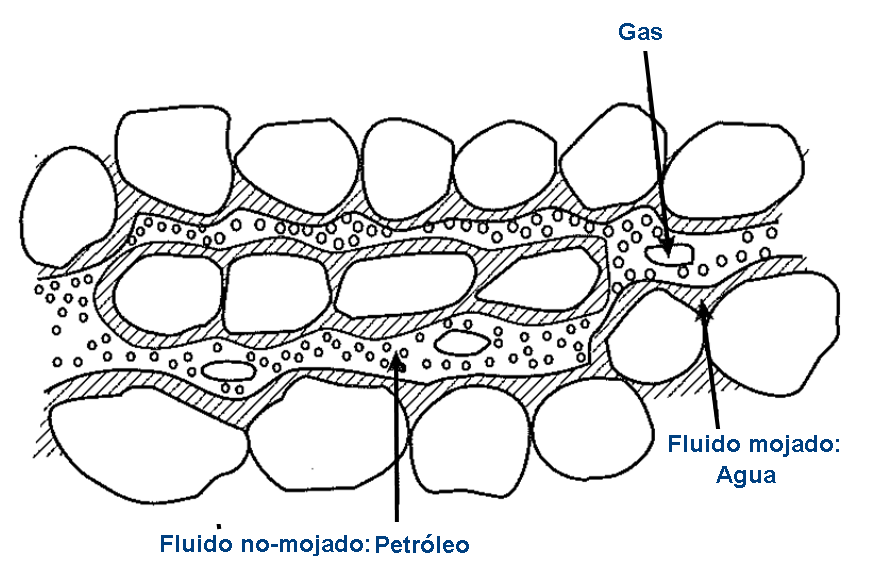
\includegraphics[width=9cm]{Imagenes/Mojabilidad.png}
\caption[Distribución de los fluidos mojado y no-mojado]{Distribución de los fluidos mojado y no-mojado. Adaptado de Rosa et al.(2006)}
\label{fig:fig33}
\end{figure}
%/////////////////////////////////////////////////////////////////////////////////////////


\textbf{G. Tasa de Saturación}
\\
En flujo multifásico no-isotérmico es importante determinar la tasa de cambio de la saturación de los fluidos. Con ayuda de la regla de la cadena se puede escribir:

%----------------------------------------------------------------------------------------
% ECUACIÓN 3.14
\begin{ceqn} 
\begin{subequations} \label{eq:equ314} 
\begin{align}
\shortintertext{Agua:} &\frac{\partial S_w}{\partial t} = \frac{\partial S_w}{\partial P_{c-ow}}\frac{\partial P_{c-ow}}{\partial t} + \frac{\partial S_w}{\partial T}\frac{\partial T}{\partial t}
\label{eq:equ326a} \\[10pt]
\shortintertext{Gas:} 			&\frac{\partial S_g}{\partial t} = \frac{\partial S_g}{\partial P_{c-go}}\frac{\partial P_{c-go}}{\partial t} + \frac{\partial S_g}{\partial T}\frac{\partial T}{\partial t}
\label{eq:equ314b} \\[10pt]
\shortintertext{Petroleo:} 			&\frac{\partial S_o}{\partial t} = -\frac{\partial S_w}{\partial t} -\frac{\partial S_g}{\partial t} \label{eq:equ314b}
\end{align}
\end{subequations} 
\end{ceqn}
%----------------------------------------------------------------------------------------
\bigskip
Utilizando la siguiente nomenclatura para las derivadas en el tiempo:

%----------------------------------------------------------------------------------------
% ECUACIÓN 3.15
\begin{ceqn} 
\begin{gather} \label{eq:equ315} 
\frac{\partial x}{\partial t} = \dot{x}
\end{gather}  
\end{ceqn}
%----------------------------------------------------------------------------------------

\bigskip
y remplazando la \textbf{Ecuación} \textbf{\ref{eq:equ313}} en la \textbf{Ecuación} \textbf{\ref{eq:equ314}} se obtiene:

%----------------------------------------------------------------------------------------
% ECUACIÓN 3.16
\begin{ceqn} 
\begin{subequations} \label{eq:equ316} 
\begin{align}
\shortintertext{Agua:}     &\dot{S_w} = S'_w\left[\dot{p_o} - \dot{p_w} \right] +S'_{wT}\dot{T} \label{eq:equ316a} \\[10pt]
\shortintertext{Gas:} 	&\dot{S_g} = S'_w\left[\dot{p_g} - \dot{p_o} \right] +S'_{gT}\dot{T} \label{eq:equ316b} \\[10pt]
\shortintertext{Petroleo:} 	&\dot{S_o} = -S'_w\left[\dot{p_o} - \dot{p_w} \right] - S'_w\left[\dot{p_g} - \dot{p_o} \right] -(S'_{wT}+S'_{gT}) \dot{T}  \label{eq:equ316c}
\end{align}
\end{subequations} 
\end{ceqn}
%----------------------------------------------------------------------------------------

donde:

%----------------------------------------------------------------------------------------
% ECUACIÓN 3.17
\begin{ceqn} 
\begin{subequations} \label{eq:equ317} 
\begin{gather}
S'_w = \frac{\partial S_w}{\partial P_{c-ow}}
\label{eq:equ317a} \\[3pt]
S'_g = -S'_w
\label{eq:equ317b} \\[3pt]
S'_{wT} = \frac{\partial S_w}{\partial T}
\label{eq:equ317c} \\[3pt]
S'_{gT} = \frac{\partial S_g}{\partial T}
\label{eq:equ317d}
\end{gather}  
\end{subequations} 
\end{ceqn}
%----------------------------------------------------------------------------------------


\textbf{H. Presión de Poros Promedio}
\\
En presencia de flujo multifásico se puede determinar la presión promedio de poros como la suma de las contribuciones de presión de poros de cada fluido, ponderadas con sus respectivas saturaciones:

%----------------------------------------------------------------------------------------
% ECUACIÓN 3.18
\begin{ceqn} 
\begin{gather} \label{eq:equ318} 
\overline{p} = S_w p_w + S_o p_o + S_g p_g
\end{gather}  
\end{ceqn}
%----------------------------------------------------------------------------------------
\\
\textbf{I. Tasa de Presión de Poros Promedio}
\\
La tasa de variación de la presión promedio de poros es función se obtiene derivando la \textbf{Ecuación} \textbf{\ref{eq:equ318}} con respecto al tiempo. Con ayuda de la regla de la cadena se obtiene:\bigskip

%----------------------------------------------------------------------------------------
% ECUACIÓN 3.19
\begin{ceqn} 
\begin{gather} \label{eq:equ319}
\dot{\overline{p}} = p_w\dot{S_w} + S_w\dot{p_w} + p_o\dot{S_o} + S_o\dot{p_o} + p_g\dot{S_g} + S_g\dot{p_g}
\end{gather}  
\end{ceqn}
%----------------------------------------------------------------------------------------
\\
Substituyendo la \textbf{Ecuación} \textbf{\ref{eq:equ316}} en la \textbf{Ecuación} \textbf{\ref{eq:equ318}} se obtiene:

%----------------------------------------------------------------------------------------
% ECUACIÓN 3.20
\begin{ceqn} 
\begin{gather}
\label{eq:equ320} 
\dot{\overline{p}} = S''_w\dot{p_w} + S''_o\dot{p_o} + S''_g\dot{p_g} + S''_T\dot{T}
\end{gather}  
\end{ceqn}
%----------------------------------------------------------------------------------------
%\bigskip

donde:

%----------------------------------------------------------------------------------------
% ECUACIÓN 3.21
\begin{ceqn} 
\begin{subequations} \label{eq:equ321} 
\begin{gather}
S''_w = S_w + P_{c-ow}S'_w 
\label{eq:equ321a} \\[3pt]
S''_o = S_o - P_{c-ow}S'_w - P_{c-go}S'_g
\label{eq:equ321b} \\[3pt]
S''_g = S_g + P_{c-go}S'_g
\label{eq:equ321c} \\[3pt]
S''_{T} = P_{c-go}S'_{gT} - P_{c-ow}S'_{wT}
\label{eq:equ321d}
\end{gather}  
\end{subequations} 
\end{ceqn}
%----------------------------------------------------------------------------------------
\\

\textbf{J. Gradiente de la Presión de Poros Promedio}
\\
De la misma forma como se determino la \textbf{Ecuación} \textbf{\ref{eq:equ320}}, se puede obtener la variación de la presión de poros promedio respecto al espacio, la cual es:

%----------------------------------------------------------------------------------------
% ECUACIÓN 3.22
\begin{ceqn} 
\begin{gather} \label{eq:equ322} 
\nabla \overline{p} = S''_w\nabla p_w + S''_o\nabla p_o + S''_g\nabla p_g
\end{gather}  
\end{ceqn}
%----------------------------------------------------------------------------------------


\textbf{K. Ecuación Geomecánica}
\\
La ecuación geomecánica es la que determina el comportamiento mecánico de un medio poroso en presencia de un cambio de los esfuerzos efectivos. Para determinarla se substituye las \textbf{Ecuaciones} \textbf{\ref{eq:equ36}} y \textbf{\ref{eq:equ311b}} en la \textbf{Ecuación} \textbf{\ref{eq:equ33}}, que resulta en:
%----------------------------------------------------------------------------------------
% ECUACIÓN 3.23

\begin{ceqn} 
\label{eq:equ323} 
\begin{gather}
\mathbf{S}^T[\mathbf{D}]\mathbf{S}\{\mathbf{u}\} - \alpha\mathbf{S}^T\{\mathbf{I}\} \overline{p} + \{\mathbf{b}\}=\{\mathbf{0}\} 
\end{gather} 
\end{ceqn}
%----------------------------------------------------------------------------------------

Definiendo:

%----------------------------------------------------------------------------------------
% ECUACIÓN 3.24
\begin{ceqn} 
\begin{subequations} \label{eq:equ324} 
\begin{gather}
\nabla = \begin{Bmatrix} 
           \frac{\partial}{\partial x} \\[5pt]
           \frac{\partial}{\partial y}
           \end{Bmatrix}
           \label{eq:equ324a} \\[10pt]
\mathbf{S}^T\{\mathbf{I}\} = \nabla
\label{eq:equ324b}
\end{gather}  
\end{subequations} 
\end{ceqn}
%----------------------------------------------------------------------------------------
donde ($\nabla$) es el operador de divergencia. Substituyendo la \textbf{Ecuación} \textbf{\ref{eq:equ322}} y \textbf{\ref{eq:equ324}} en la \textbf{Ecuación} \textbf{\ref{eq:equ323}}, reordenando y simplificando se obtiene:\\

%----------------------------------------------------------------------------------------
% ECUACIÓN 3.25
\hfsetfillcolor{black!20}
\hfsetbordercolor{black}
\begin{ceqn} 
\begin{gather} \label{eq:equ325}
\tikzmarkin{equ325}(0.3,-0.5)(-0.3,0.6)
\mathbf{S}^T[\mathbf{D}]\mathbf{S}\{\mathbf{u}\} - 
\alpha S''_w\nabla p_w - \alpha S''_o\nabla p_o -  \alpha S''_g\nabla p_g + - \frac{\beta_s}{3}[\mathbf{D}]\{\mathbf{I}\} \nabla T  + \{\mathbf{b}\} = \{\mathbf{0}\}
\tikzmarkend{equ325}
\end{gather}  
\end{ceqn}
%----------------------------------------------------------------------------------------
\\
La \textbf{Ecuación} \textbf{\ref{eq:equ325}} es la (\textit{EDP}) que gobierna el comportamiento geomecánico del modelo (\textit{MTA-THG}). Esta ecuación tiene cinco incógnitas el vector de desplazamiento, la presión de poros de cada fluido y la temperatura.\vspace{0.7cm}



%........................................................................................
% TITULO DE LA SUBSECCIÓN 3.2.2
\subsection{Modelo de Flujo (\textit{MTA-THG})}~\hypertarget{sec:sec322}{}
\label{sec:sec322}


El movimiento de fluidos a través de medios porosos está gobernado por las mismas leyes fundamentales que rigen su movimiento en otros medios, como la atmósfera, redes de tuberías o fuentes de agua. Esas leyes están basadas en la conservación de la masa, momento y energía \cite{Aziz1979PetroleumSimulation}. Para determinar el modelo de flujo se va utilizar el \textit{Modelo Black-Oil} y el procedimiento utilizado por Pao et al.(2001). En el Apéndice A, se hace todo el desarrollo necesario para determinar la (\textit{EDP}) que rige el comportamiento de flujo para cada uno de los fluidos presentes en el medio poroso. Esa ecuación se expresa:\\

%----------------------------------------------------------------------------------------
% ECUACIÓN 3.26

\begin{ceqn} 
\label{eq:equ326} 
\begin{gather}
\nabla^T \left[ T_m \nabla[p_i - g\rho_I]\right] =
\alpha \lambda_f\{\mathbf{I}\}\mathbf{S}\{\dot{u}\} + \lambda_f \frac{\alpha - \phi}{K_m}\dot{\overline{p}} - (\alpha - \phi)\frac{S_i}{B_i}\frac{\beta_s}{3}\dot{T}
+ \phi \dot{\lambda_f}
\end{gather} 
\end{ceqn}
%----------------------------------------------------------------------------------------
\newpage
donde:
%----------------------------------------------------------------------------------------
% ECUACIÓN 3.27
\begin{ceqn} 
\begin{subequations} \label{eq:equ327} 
\begin{gather}
T_m = [\mathbf{K}] \left[ \frac{k_{ri}}{\mu_{i} B_{i}} + R_{si} \frac{k_{ri}}{\mu_{i} B_{i}} \right]      
\label{eq:equ327a} \\[10pt]
\lambda_f = \frac{S_i}{B_i} + R_{si}\frac{S_i}{B_i}
\label{eq:equ327b}
\end{gather}  
\end{subequations} 
\end{ceqn}
%----------------------------------------------------------------------------------------


donde ($\mathbf{K}$) es el tensor de permeabilidad intrínseca, ($k_{ri}$) es la permeabilidad relativa del fluido $i$, ($\mu_i$) es la viscosidad dinámica del fluido $i$, ($B_i$) es el factor volumen-formación del fluido $i$, ($g$) es la aceleración de la gravedad, ($\rho_I$) es la densidad del fluido $i$ en condiciones estándar \footnote{Según}, ($R_{si}$) es la razón de solubilidad del fluido $i$,el subíndice ($i$) indica los fluidos que saturan el medio (i.e. gas, petroleo, agua)\bigskip

\textbf{A. Ecuación de flujo para el agua}
\\
Para aplicar la \textbf{Ecuación} \textbf{\ref{eq:equ326}} a la fase del agua se debe asumir lo siguiente: (1) El agua no tiene gas disuelto ($R_{sw} = 0$); (2) El agua en condiciones de reservorio es compresible ($B_{w} \neq 0$). Por lo tanto:\bigskip

%----------------------------------------------------------------------------------------
% ECUACIÓN 3.28

\begin{ceqn} 
\label{eq:equ328} 
\begin{gather}
\nabla^T \left[ \frac{[\mathbf{K}] k_{rw}}{\mu_{w}B_{w}} \nabla[p_w - g\rho_{W}] \right] =
\alpha \frac{S_w}{B_w}\{\mathbf{I}\}\mathbf{S}\{\dot{u}\} + \frac{S_w}{B_w} \frac{(\alpha - \phi)}{K_m}\dot{\overline{p}} - (\alpha - \phi)\frac{S_w}{B_w}\frac{\beta_s}{3}\dot{T}
+ \phi \frac{\partial}{\partial t}\left(\frac{S_w}{B_w}\right)
\end{gather} 
\end{ceqn}
%----------------------------------------------------------------------------------------

\bigskip
El ultimo termino de la \textbf{Ecuación} \textbf{\ref{eq:equ328}} se determina por medio de la regla de la cadena resultando en:

%----------------------------------------------------------------------------------------
% ECUACIÓN 3.29

\begin{ceqn} 
\begin{subequations} \label{eq:equ329} 
\begin{gather}
\phi \frac{\partial}{\partial t}\left(\frac{S_w}{B_w}\right) = \frac{\phi}{B_w} \dot{S_w} + \phi S_w \frac{\partial (1/B_w) }{\partial pw}\ \dot{p_w}
+ \phi S_w \frac{\partial (1/B_w) }{\partial T}\ \dot{T}
\label{eq:equ329a} \\[10pt]
\phi \frac{\partial}{\partial t}\left(\frac{S_w}{B_w}\right) = \frac{\phi}{B_w} \dot{S_w} + \phi S_w B'_{wp} \ \dot{p_w}
+ \phi S_w B'_{wT} \ \dot{T}
\label{eq:equ329b}
\end{gather}
\end{subequations} 
\end{ceqn}
%----------------------------------------------------------------------------------------

\bigskip
Reemplazando las \textbf{Ecuaciones} \textbf{\ref{eq:equ320}} y \textbf{\ref{eq:equ329}} en la \textbf{Ecuación} \textbf{\ref{eq:equ328}} y reordenando se obtiene:

%----------------------------------------------------------------------------------------
% ECUACIÓN 3.30
\hfsetfillcolor{black!20}
\hfsetbordercolor{black}
\begin{ceqn} 
\label{eq:equ330} 
\begin{gather}
\begin{multlined}
\tikzmarkin{equ330}(0.25,-0.5)(-0.25,0.7)
\nabla^T \left[ \frac{[\mathbf{K}] k_{rw}}{\mu_{w}B_{w}} \nabla[p_w - g\rho_{w,std}] \right] =
\left[\frac{S_w}{B_w} \frac{(\alpha - \phi)}{K_m}S''_w - \frac{\phi}{B_w} S'_w + \phi S_w B'_{wp}   \right]\dot{p_w}\\[10pt] 
+ \left[\frac{S_w}{B_w} \frac{(\alpha - \phi)}{K_m}S''_o + \frac{\phi}{B_w} S'_w\right]\dot{p_o} + \left[\frac{S_w}{B_w} \frac{(\alpha - \phi)}{K_m}S''_g \right]\dot{p_g}  \\[10pt]
+ \alpha \frac{S_w}{B_w}\{\mathbf{I}\}\mathbf{S}\{\dot{u}\} + \left[ \frac{S_w}{B_w}\frac{(\alpha - \phi)}{K_m}S''_{T} + \frac{\phi}{B_w} S'_{wT} + \phi S_w B'_{wT} - \frac{S_w}{B_w}(\alpha - \phi)\beta_s  \right]\dot{T}
\tikzmarkend{equ330} \label{eq:equ330a}
\end{multlined}
\end{gather}  
\end{ceqn}
%----------------------------------------------------------------------------------------




% %----------------------------------------------------------------------------------------
% % ECUACIÓN 3.15
% \begin{ceqn} 
% \begin{subequations} \label{eq:equ315} 
% \begin{gather}
% \frac{\partial w_{xx}}{\partial x} + \frac{\partial \epsilon_{xx}}{\partial t} + \frac{\phi}{K_f}\frac{\partial p}{\partial t} + \frac{(1-\phi)}{K_m}\frac{\partial p}{\partial t} - \frac{K}{K_m}\left[\frac{\partial \epsilon_{xx}}{\partial t} + \frac{1}{K_m}\frac{\partial p}{\partial t}\right]= 0
% \label{eq:equ315a}\\[10pt]
% \frac{\partial w_{yy}}{\partial y} + \frac{\partial \epsilon_{yy}}{\partial t} + \frac{\phi}{K_f}\frac{\partial p}{\partial t} + \frac{(1-\phi)}{K_m}\frac{\partial p}{\partial t} - \frac{K}{K_m}\left[\frac{\partial \epsilon_{yy}}{\partial t} + \frac{1}{K_m}\frac{\partial p}{\partial t}\right] = 0
% \label{eq:equ315b}\\[10pt]
% \frac{\partial w_{zz}}{\partial z} + \frac{\partial \epsilon_{zz}}{\partial t} + \frac{\phi}{K_f}\frac{\partial p}{\partial t} + \frac{(1-\phi)}{K_m}\frac{\partial p}{\partial t} - \frac{K}{K_m}\left[\frac{\partial \epsilon_{zz}}{\partial t} + \frac{1}{K_m}\frac{\partial p}{\partial t}\right] = 0
% \label{eq:equ315c}
% \end{gather}  
% \end{subequations} 
% \end{ceqn}
% %----------------------------------------------------------------------------------------
% \\
% donde ($\mathbf{w}$) son las velocidades de infiltración del fluido que satura el medio en las tres direcciones, ($K_f$) es el módulo de compresibilidad volumétrica del fluido, ($K$) es el módulo de compresibilidad volumétrica del medio, ($\phi$) es la porosidad del medio. De la anterior ecuación se puede definir:

% %----------------------------------------------------------------------------------------
% % ECUACIÓN 3.16
% \begin{ceqn} 
% \begin{subequations} \label{eq:equ316} 
% \begin{gather}
% \{\mathbf{w}\} = \begin{Bmatrix} 
%                 w_{xx}\\[5pt]
%                 w_{yy}\\[5pt]
%                 w_{zz}
%                 \end{Bmatrix}
%                 \label{eq:equ316a}\\[10pt]
% K = \frac{\{\mathbf{I}\}[\mathbf{D}]\{\mathbf{I}\}^T}{9} \label{eq:equ316b}
% \end{gather}  
% \end{subequations} 
% \end{ceqn}
% %----------------------------------------------------------------------------------------
% \\
% Substituyendo las \textbf{Ecuaciones} \textbf{\ref{eq:equ316}} en la \textbf{Ecuación} \textbf{\ref{eq:equ315}}, reorganizando se obtiene:

% %----------------------------------------------------------------------------------------
% % ECUACIÓN 3.17
% \begin{ceqn}
% \begin{subequations}\label{eq:equ317}
% \begin{gather}
% \nabla^T \{\mathbf{w}\} + \left[1-\frac{\{\mathbf{I}\}[\mathbf{D}]\{\mathbf{I}\}^T}{9K_m}\right]\frac{\partial \{\mathbf{I}\}^T \{\mathbf{\epsilon}\}}{\partial t} +\left[\frac{\phi}{K_f}+\frac{(1-\phi)}{K_m}-\frac{\{\mathbf{I}\}[\mathbf{D}]\{\mathbf{I}\}^T}{(3K_{m})^{2}}\right]\frac{\partial p}{\partial t} = 0 \label{eq:equ317a}\\[10pt]
% \nabla^T \{\mathbf{w}\} + \alpha\frac{\partial \{\mathbf{I}\}^T \{\mathbf{\epsilon}\}}{\partial t} +\left[\frac{\phi}{K_f}+\frac{(\alpha-\phi)}{K_m}\right]\frac{\partial p}{\partial t} = 0 \label{eq:equ317a}
% \end{gather}
% \end{subequations} 
% \end{ceqn}
% %----------------------------------------------------------------------------------------
% \\
% donde ($\mathbf{w}$) es el vector de velocidad de infiltración. Esta ecuación es la que rige el flujo en medios porosos saturados con características isotópicas y elásticas. Se tienen dos incógnitas, el campo de desplazamientos y la presión de poros del fluido que satura el medio. La ley de Darcy \cite{Zienkiewicz1999ComputationalGeomechanics} establece que:

% %----------------------------------------------------------------------------------------
% % ECUACIÓN 3.18
% \begin{ceqn} 
% \begin{subequations} \label{eq:equ318} 
% \begin{gather}
% w_{xx} = -k_{xx}\frac{\partial h}{\partial x}
% \label{eq:equ318a}\\[10pt]
% w_{yy} = -k_{yy}\frac{\partial h}{\partial y}
% \label{eq:equ318b}\\[10pt]
% w_{zz} = -k_{zz}\frac{\partial h}{\partial z}
% \label{eq:equ318c}
% \end{gather}  
% \end{subequations} 
% \end{ceqn}
% %----------------------------------------------------------------------------------------

% donde ($h$) es la carga total de energía, ($k$) es la conductividad hidráulica.\bigskip


% Definiendo: 

% %----------------------------------------------------------------------------------------
% % ECUACIÓN 3.19
% \begin{ceqn} 
% \begin{subequations} \label{eq:equ319} 
% \begin{gather}
% k = \frac{\gamma}{\mu} \overline{K}
% \label{eq:equ319a}\\[10pt]
% h = \frac{p}{\gamma} + \frac{w^2}{2g} + z
% \label{eq:equ319b}
% \end{gather}  
% \end{subequations} 
% \end{ceqn}
% %----------------------------------------------------------------------------------------

% donde ($\gamma$)  y ($\mu$) son el peso especifico y la viscosidad dinámica del fluido de saturación respectivamente, ($\overline{K}$) es la permeabilidad absoluta del medio poroso. Reemplazando la  \textbf{Ecuación} \textbf{\ref{eq:equ319}} en la \textbf{Ecuación} \textbf{\ref{eq:equ318}} y despreciando el aporte de la carga de velocidad, se obtiene: 

% %----------------------------------------------------------------------------------------
% % ECUACIÓN 3.20
% \begin{ceqn} 
% \begin{subequations} \label{eq:equ320} 
% \begin{gather}
% \{\mathbf{w}\}=-\frac{[\mathbf{\overline{K}}]}{\mu} (\nabla p + \rho \mathbf{g}\nabla z)
% \label{eq:equ320a}\\[10pt]
% [\mathbf{\overline{K}}]=\begin{bmatrix} 
% k_{xx} & 0 & 0 \\[3pt]
% 0 & k_{yy} & 0 \\[3pt]
% 0 & 0 & k_{zz} 
% \end{bmatrix}
% \label{eq:equ320b}\\[10pt]
% \nabla z = \frac{\partial z}{\partial x} + \frac{\partial z}{\partial y} +\frac{\partial z}{\partial z} = 1
% \label{eq:equ320c}
% \end{gather}  
% \end{subequations} 
% \end{ceqn}
% %----------------------------------------------------------------------------------------
% donde ($\mathbf{\overline{K}}$) es el tensor de permeabilidad. Reemplazando la \textbf{Ecuación} \textbf{\ref{eq:equ320}}  en la \textbf{Ecuación} \textbf{\ref{eq:equ317}} se obtiene:

% %----------------------------------------------------------------------------------------
% % ECUACIÓN 3.21
% \begin{ceqn}
% \begin{gather}\label{eq:equ321}
% \normalsize{\nabla^T \left[\frac{[\mathbf{\overline{K}}]}{\mu}(\nabla p + \rho \mathbf{g})\right] = \alpha\frac{\partial \{\mathbf{I}\}\mathbf{S}\{\mathbf{u}\}}{\partial t} +\left[\frac{\phi}{K_f}+\frac{(\alpha-\phi)}{K_m}\right]\frac{\partial p}{\partial t}}
% \end{gather}   
% \end{ceqn}
% %----------------------------------------------------------------------------------------

% Definiendo:
% %----------------------------------------------------------------------------------------
% % ECUACIÓN 3.22
% \begin{ceqn} 
% \begin{subequations} \label{eq:equ322} 
% \begin{gather}
% \{\mathbf{\dot{u}}\} = \frac{\partial \{\mathbf{u}\}}{\partial t}
% \label{eq:equ322a}\\[10pt]
% \dot{p} = \frac{\partial p}{\partial t}
% \label{eq:equ322b}\\[10pt]
% \frac{1}{Q} = \frac{\phi}{K_f}+\frac{(\alpha-\phi)}{K_m}
% \label{eq:equ322c}
% \end{gather}  
% \end{subequations} 
% \end{ceqn}
% %----------------------------------------------------------------------------------------

% La \textbf{Ecuación} \textbf{\ref{eq:equ321}} se puede escribir:
% %----------------------------------------------------------------------------------------
% % ECUACIÓN 3.23
% \hfsetfillcolor{black!20}
% \hfsetbordercolor{black}
% \begin{ceqn}
% \begin{gather}\label{eq:equ323}
% \tikzmarkin{equ323}(0.5,-0.7)(-0.5,0.9)
% \nabla^T \left[\frac{[\mathbf{\overline{K}}]}{\mu}(\nabla p + \rho \mathbf{g})\right] = \alpha\{\mathbf{I}\}\mathbf{S}\{\mathbf{\dot{u}}\} + \frac{1}{Q}\ \dot{p}
% \tikzmarkend{equ323}
% \end{gather}   
% \end{ceqn}
% %----------------------------------------------------------------------------------------
% \\
% Esta ecuación rige el flujo en un medio poroso saturado. Esta ecuación rige el comportamiento de medios porosos tanto elásticos como elastoplásticos. En conjunto con la \textbf{Ecuación} \textbf{\ref{eq:equ314}} se tiene el sistema de ecuaciones del modelo flujo-geomecánico acoplado.\bigskip

% Para el caso particular de Elasticidad e Isotropía se debe reemplazar la \textbf{Ecuación} \textbf{\ref{eq:equ323c}} en la \textbf{Ecuación} \textbf{\ref{eq:equ326}} y se obtiene:\bigskip

% %----------------------------------------------------------------------------------------
% % ECUACIÓN 3.27
% \hfsetfillcolor{black!20}
% \hfsetbordercolor{black}
% \begin{ceqn} %\label{eq:equ327}
% \begin{gather}\label{eq:equ327}
% \tikzmarkin{equ327}(0.5,-0.7)(-0.5,0.9)
% \normalsize{\nabla^T \left[\frac{[\mathbf{K}]}{\mu}\nabla p\right] = \left[1-\frac{K}{K_{m}}\right]\frac{\partial \nabla^T \{\mathbf{u}\}}{\partial t} +\left[\frac{\phi}{K_f}+\frac{(1-\phi)}{K_m}- \frac{K}{K_{m}^{2}}\right]\frac{\partial p}{\partial t}}
% \tikzmarkend{equ327}
% \end{gather}   
% \end{ceqn}
% %----------------------------------------------------------------------------------------
\bigskip




%........................................................................................
% TITULO DE LA SUBSECCIÓN 3.2.2
\subsection{Medio Poroso Parcialmente Saturado}~\hypertarget{sec:sec322}{}
\label{sec:sec322}

Un medio poroso parcialmente saturado tiene en sus vacíos dos o más fluidos que saturan el medio. Por ejemplo, un suelo residual que se caracteriza por estar parcialmente saturado, en sus vacíos tiene agua y aire. Un reservorio de petróleo se caracteriza porque en los vacíos de la roca que lo conforma pueden existir hasta tres tipos de fluidos: Gas, petróleo y agua\bigskip

En esta investigación se tiene como alcance el estudio de medios porosos en presencia de flujo bifásico. Por lo tanto, el modelo será función de un fluido que moja preferencialmente el medio poroso, que se conoce como \textit{fluido mojado}, y un fluido con una menor tendencia de mojar preferencialmente los solidos del medio, que se conoce como el \textit{fluido no-mojado}.\bigskip

En un reservorio de petróleo se sabe que el agua moja preferencialmente la roca en la mayoría de los casos, como se ve en la \textbf{Figura} \ref{fig:fig32}. El gas se mantiene en los canales centrales de los poros puesto que es un fluido que presenta la menor tendencia de mojar preferencialmente la roca. El agua estaría en las paredes de los poros junto a las partículas sólidas de la roca. El petróleo por ser un fluido intermediario en términos de mojabilidad, estaría localizado entre el agua y el gas.\bigskip

%////////////////////////////////////////////////////////////////////////////////////////
% Figura 3.2
\begin{figure}[!ht]
\centering
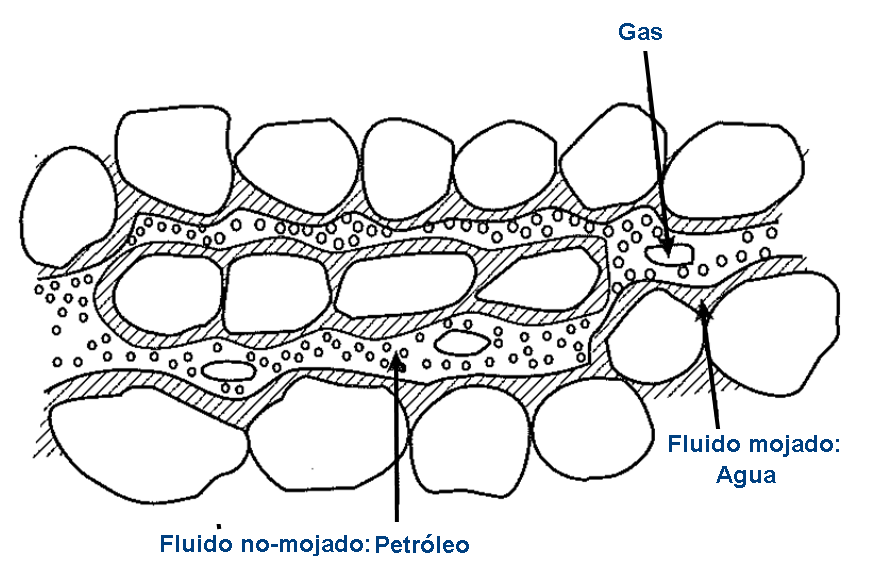
\includegraphics[width=8cm]{Imagenes/Mojabilidad.png}
\caption[Distribución de los fluidos mojado y no-mojado]{Distribución de los fluidos mojado y no-mojado. Modificado de Rosa et al.(2006) \cite{Rosa2006EngenhariaPetroleo}}
\label{fig:fig32}
\end{figure}
%/////////////////////////////////////////////////////////////////////////////////////////

En un suelo parcialmente saturado, es el agua quien moja preferencialmente los sólidos del suelo, y por eso se le denomina al agua como el \textit{fluido mojado}. El aire en los vacíos del suelo presenta una menor tendencia de mojar los sólidos del suelo y por eso se le considera como el \textit{fluido no-mojado}.\newpage



%........................................................................................
% TITULO DE LA SUBSECCIÓN 3.2.2.1
\subsubsection{Definiciones Iniciales}~\hypertarget{sec:sec3221}{}
\label{sec:sec3221}

Para empezar la determinación del modelo geomecánico de un medio poroso parcialmente saturado, se deben hacer primero unas definiciones.\bigskip


\textbf{A. Saturación}
\\
El grado de saturación ($S$) se define como la razón entre el volumen de vacíos y el volumen total del medio poroso. Para un suelo saturado, el grado de saturación del fluido es 100\%. Para un medio parcialmente saturado, el grado de saturación es la suma de la saturación del \textit{fluido mojado} más la saturación del \textit{fluido no-mojado}:

%----------------------------------------------------------------------------------------
% ECUACIÓN 3.24
\begin{ceqn} 
\begin{gather} \label{eq:equ324} 
S_w + S_n = 1
\end{gather}  
\end{ceqn}
%----------------------------------------------------------------------------------------
\\
donde ($S_w$) es la saturación del \textit{fluido mojado} y ($S_n$) es la saturación del fluido \textit{fluido no-mojado}.\bigskip


\textbf{B. Presión Capilar}
\\
Cuando se habla de flujo bifásico se debe tener en cuenta la presión capilar ($P_c$). La presión capilar es la diferencia de presión a través de la interfase que separa dos fluidos inmiscibles, cuando se ponen en contacto en un medio poroso. Con ayuda de la presión capilar se establece la relación que existe entre la presión de poros del \textit{fluido mojado} y la del fluido \textit{fluido no-mojado}:

%----------------------------------------------------------------------------------------
% ECUACIÓN 3.25
\begin{ceqn} 
\begin{gather} \label{eq:equ325} 
P_c = p_n - p_w
\end{gather}  
\end{ceqn}
%----------------------------------------------------------------------------------------
\\
donde ($p_w$) es la presión de poros del fluido \textit{fluido mojado} y ($p_n$) es la presión de poros del fluido \textit{fluido no-mojado}, ($P_c$) es la presión capilar.\bigskip


\textbf{C. Tasa de Saturación}
\\
En flujo bifásico es importante determinar cuál es la tasa de cambio de la saturación de los fluidos mojado y no-mojado, referente al tiempo. Con ayuda de la regla de la cadena se puede escribir:

%----------------------------------------------------------------------------------------
% ECUACIÓN 3.26
\begin{ceqn} 
\begin{subequations} \label{eq:equ326} 
\begin{align}
\shortintertext{Fluido mojado:} &\frac{\partial S_w}{\partial t} = \frac{\partial S_w}{\partial P_c}\frac{\partial P_c}{\partial t} \label{eq:equ326a} \\[10pt]
\shortintertext{Fluido no-mojado:} 			&\frac{\partial S_n}{\partial t} = \frac{\partial S_n}{\partial P_c}\frac{\partial P_c}{\partial t} \label{eq:equ326b}
\end{align}
\end{subequations} 
\end{ceqn}
%----------------------------------------------------------------------------------------

\bigskip
Remplazando la \textbf{Ecuación} \textbf{\ref{eq:equ325}} en la \textbf{Ecuación} \textbf{\ref{eq:equ326}} se obtiene:

%----------------------------------------------------------------------------------------
% ECUACIÓN 3.27
\begin{ceqn} 
\begin{subequations} \label{eq:equ327} 
\begin{align}
\shortintertext{Fluido mojado:}     &\frac{\partial S_w}{\partial t} = \frac{\partial S_w}{\partial P_c}\left[\frac{\partial p_n}{\partial t}-\frac{\partial p_w}{\partial t}\right] = S'_w\left[\frac{\partial p_n}{\partial t}-\frac{\partial p_w}{\partial t}\right] \label{eq:equ327a} \\[10pt]
\shortintertext{Fluido no-mojado:} 	&\frac{\partial S_n}{\partial t} = \frac{\partial S_n}{\partial P_c}\left[\frac{\partial p_w}{\partial t}-\frac{\partial p_w}{\partial t}\right] = -S'_w\left[\frac{\partial p_w}{\partial t}-\frac{\partial p_w}{\partial t}\right] \label{eq:equ327b}
\end{align}
\end{subequations} 
\end{ceqn}
%----------------------------------------------------------------------------------------

\bigskip
Utilizando la siguiente nomenclatura para las derivadas en el tiempo:

%----------------------------------------------------------------------------------------
% ECUACIÓN 3.28
\begin{ceqn} 
\begin{gather} \label{eq:equ328} 
\frac{\partial x}{\partial t} = \dot{x}
\end{gather}  
\end{ceqn}
%----------------------------------------------------------------------------------------

la \textbf{Ecuación} \textbf{\ref{eq:equ327}} se puede escribir:

%----------------------------------------------------------------------------------------
% ECUACIÓN 3.29
\begin{ceqn} 
\begin{subequations} \label{eq:equ329} 
%\begin{gather}
\begin{align}
\shortintertext{Fluido mojado:}     &\dot{S_w} = S'_w\left[\dot{p_n}-\dot{ p_w}\right] \label{eq:equ329a} \\[10pt]
\shortintertext{Fluido no-mojado:} 	&\dot{S_n} = -S'_w\left[\dot{p_n}-\dot{ p_w}\right] \label{eq:equ329b}
\end{align}
%\end{gather}  
\end{subequations} 
\end{ceqn}
%----------------------------------------------------------------------------------------
%\bigskip

\textbf{D. Presión de Poros Promedio}
\\
En presencia de flujo bifásico se puede determinar la presión promedio de poros como la suma de las contribuciones de presión de poros de cada fluido, ponderadas con sus respectivas saturaciones:

%----------------------------------------------------------------------------------------
% ECUACIÓN 3.30
\begin{ceqn} 
\begin{gather} \label{eq:equ330} 
\overline{p} = S_w p_w + S_n p_n
\end{gather}  
\end{ceqn}
%----------------------------------------------------------------------------------------
\\
\textbf{E. Tasa de Presión de Poros Promedio}
\\
Como se puede ver en la \textbf{Ecuación} \textbf{\ref{eq:equ329}} es necesario determinar la tasa de variación de la presión de poros. Para tener en cuenta las presiones de poros de los \textit{fluidos mojado y no-mojado} es necesario derivar la \textbf{Ecuación} \textbf{\ref{eq:equ330}} con respecto al tiempo. Con ayuda de la regla de la cadena se obtiene:\bigskip

%----------------------------------------------------------------------------------------
% ECUACIÓN 3.31
\begin{ceqn} 
\begin{gather} \label{eq:equ331}
\dot{\overline{p}} = p_w\dot{S_w} + S_w\dot{p_w} + p_n\dot{S_n} + S_n\dot{p_n}
\end{gather}  
\end{ceqn}
%----------------------------------------------------------------------------------------
\\
Substituyendo la \textbf{Ecuación} \textbf{\ref{eq:equ329}} en la \textbf{Ecuación} \textbf{\ref{eq:equ331}} se obtiene:

%----------------------------------------------------------------------------------------
% ECUACIÓN 3.32
\begin{ceqn} 
\begin{subequations} \label{eq:equ332} 
\begin{gather}
\dot{\overline{p}} = p_w S'_w\left[\dot{p_n}-\dot{p_w}\right] + S_w\dot{p_w}  - p_n S'_w\left[\dot{p_n}-\dot{p_w}\right] + S_n\dot{p_n} \label{eq:equ332a} \\[12pt]
\dot{\overline{p}} = S''_w\dot{p_w} + S''_n\dot{p_n}  \label{eq:equ332b}
\end{gather}  
\end{subequations} 
\end{ceqn}
%----------------------------------------------------------------------------------------
%\bigskip

\textbf{F. Gradiente de la Presión de Poros Promedio}
\\
De la misma forma como se determino la \textbf{Ecuación} \textbf{\ref{eq:equ332b}}, se puede obtener la variación de la presión de poros promedio respecto al espacio:

%----------------------------------------------------------------------------------------
% ECUACIÓN 3.33
\begin{ceqn} 
\begin{gather} \label{eq:equ333} 
\nabla \overline{p} = S''_w\nabla p_w + S''_n\nabla p_n
\end{gather}  
\end{ceqn}
%----------------------------------------------------------------------------------------


\bigskip
\textbf{G. Relación entre la Presión Capilar y la Saturación del fluido mojado ($P_c$ vs. $S_w$)}
\\
Finalmente



\bigskip
\textbf{H. Permeabilidades Relativas}
\\
Finalmente





%........................................................................................
% TITULO DE LA SUBSECCIÓN 3.2.2.2
\subsubsection{Modelo Geomecánico}~\hypertarget{sec:sec3222}{}
\label{sec:sec3221}


Para obtener el modelo geomecánico para un medio poroso parcialmente saturado. Se substituye la \textbf{Ecuación} \textbf{\ref{eq:equ333}} en la \textbf{Ecuación} \textbf{\ref{eq:equ314}} y se obtiene:\bigskip

%----------------------------------------------------------------------------------------
% ECUACIÓN 3.34

\begin{ceqn} 
\begin{subequations} \label{eq:equ334} 
\begin{gather}
\tikzmarkin{equ335}(0.5,-0.5)(-0.5,0.7)
\normalsize{\mathbf{S}^T[\mathbf{D}]\mathbf{S}\{\mathbf{u}\} - 
\alpha S''_w\nabla p_w + \alpha S''_n\nabla p_n + \{\mathbf{b}\} = \{\mathbf{0}\}}
\tikzmarkend{equ335}\label{eq:equ334a} \\[12pt]
S''_w = S_w + P_c\frac{\partial S_w}{\partial P_c}  \label{eq:equ334b} \\[12pt]
S''_n = S_n - P_c\frac{\partial S_n}{\partial P_c}  \label{eq:equ334c}
\end{gather}
\end{subequations} 
\end{ceqn}
%----------------------------------------------------------------------------------------
\\
Esta ecuación gobierna el comportamiento mecánico de medios porosos parcialmente saturados en presencia de flujo bifásico. Las incógnitas de esta ecuación sigue siendo el campo de desplazamientos, pero se suma ahora la presión de poros del \textit{fluido mojado} ($p_w$), la presión de poros del \textit{fluido no-mojado} ($p_n$), la saturación del \textit{fluido mojado} ($S_w$) y la saturación del \textit{fluido no-mojado} ($S_n$). Como hay mas incógnitas que ecuaciones, para solucionar el problema se debe adoptar una técnica implícita o explicita en el modelo numérico que solucione este inconveniente.\bigskip


% \textbf{H. Modelo Geomecánico Medio Poroso Parcialmente Saturado - Caso Elástico}
% \\
% Para el caso especial que el medio poroso sea elástico e isotrópico la \textbf{Ecuación} \textbf{\ref{eq:equ338}} se puede escribir de la siguiente forma:\bigskip


% %----------------------------------------------------------------------------------------
% % ECUACIÓN 3.39
% \hfsetfillcolor{black!20}
% \hfsetbordercolor{black}
% \begin{ceqn} 
% \begin{subequations} \label{eq:equ339} 
% \begin{gather}
% %\begin{align}
% \tikzmarkin{equ336}(0.25,-0.7)(-0.25,0.9)
% \normalsize{G\nabla^2 \{\mathbf{u}\}
% +\frac{G}{1-2\nu} \nabla\left( \nabla\cdot \{\mathbf{u}\}\right)
% - \alpha S''_w\nabla p_w - \alpha S''_n\nabla p_n + \{\mathbf{b}\} = \{\mathbf{0}\}}
% \tikzmarkend{equ336}\label{eq:equ339a} \\[12pt]
% S''_w = S_w + P_c\frac{\partial S_w}{\partial P_c}  \label{eq:equ339b} \\[12pt]
% S''_n = S_n - P_c\frac{\partial S_n}{\partial P_c}  \label{eq:equ339c} \\[12pt]
% P_c = \mathnormal{f}(S_w) = p_n - p_w  \label{eq:equ339d} 
% %\end{align}
% \end{gather}  
% \end{subequations} 
% \end{ceqn}
% %----------------------------------------------------------------------------------------


%........................................................................................
% TITULO DE LA SUBSECCIÓN 3.2.2.3
\subsubsection{Modelo de Flujo}~\hypertarget{sec:sec3323}{}
\label{sec:sec3323}

Para obtener el modelo de flujo bifásico se utiliza la misma metodología usada por Zienkiewicz et al.(1999) \cite{Zienkiewicz1999ComputationalGeomechanics}, para determinar la tasa de acumulación de fluidos en un medio poroso, como ya se mostró en la determinación de la \textbf{Ecuación} \textbf{\ref{eq:equ315}}. Para un medio poroso parcialmente saturado la tasa de acumulación de fluido mojado se puede expresar de la siguiente forma:\bigskip

%----------------------------------------------------------------------------------------
% ECUACIÓN 3.40
\begin{ceqn} %\label{eq:equ340}
\begin{gather}\label{eq:equ340}
\nabla^T \{\mathbf{w}_{\pi}\} + S_{\pi} \frac{\alpha - \phi}{K_m}\frac{\partial \overline{p}}{\partial t} + \phi\frac{\partial S_{\pi}}{\partial t} + \alpha S_{\pi}\frac{\partial\mathbf{I}^T \{\mathbf{\epsilon}\}}{\partial t} + S_{\pi}\frac{\phi}{K_{\pi}}\frac{\partial p_{\pi}}{\partial t} = 0
\end{gather}   
\end{ceqn}
%----------------------------------------------------------------------------------------
\bigskip

Esta ecuación aplica para cualquier tipo de fluido. Aplicando esta ecuación al fluido mojado ($w$) y cambiando la terminología de las derivadas parciales con respecto al tiempo como en la \textbf{Ecuación} \textbf{\ref{eq:equ332}}, se obtiene:

%----------------------------------------------------------------------------------------
% ECUACIÓN 3.41
\begin{ceqn} %\label{eq:equ341}
\begin{gather}\label{eq:equ341}
\nabla^T \{\mathbf{w}_{w}\} + S_{w} \frac{\alpha - \phi}{K_m}\dot{\overline{p}}+ \phi\dot{S_{w}} + \alpha S_{w}\mathbf{I}^T \dot{\{\mathbf{\epsilon}\}} + S_{w}\frac{\phi}{K_{w}}\dot{p_{w}} = 0
\end{gather}   
\end{ceqn}
%----------------------------------------------------------------------------------------
\bigskip
y para el fluido no-mojado se obtiene:

%----------------------------------------------------------------------------------------
% ECUACIÓN 3.42
\begin{ceqn} %\label{eq:equ342}
\begin{gather}\label{eq:equ342}
\nabla^T \{\mathbf{w}_{n}\} + S_{n} \frac{\alpha - \phi}{K_m}\dot{\overline{p}}+ \phi\dot{S_{n}} + \alpha S_{n}\mathbf{I}^T \dot{\{\mathbf{\epsilon}\}} + S_{n}\frac{\phi}{K_{n}}\dot{p_{n}} = 0
\end{gather}   
\end{ceqn}
%----------------------------------------------------------------------------------------
\bigskip
La ley de Darcy \cite{Zienkiewicz1999ComputationalGeomechanics} para flujo bifásico establece:

%----------------------------------------------------------------------------------------
% ECUACIÓN 3.43
\begin{ceqn} 
\begin{subequations} \label{eq:equ343} 
\begin{gather}
%\begin{align}
\normalsize{\{\mathbf{w}_{\pi}\} = \frac{[\mathbf{k}] k_{r\pi}}{\mu_{\pi}}\nabla p_{\pi}} \label{eq:equ343a}\\[10pt]
\normalsize{[\mathbf{k}]=\begin{bmatrix} 
k_{x} & 0\\[1em]
0 & k_{y}
\end{bmatrix} } \label{eq:equ343b}
%\end{align}
\end{gather}  
\end{subequations} 
\end{ceqn}
%----------------------------------------------------------------------------------------

donde ($\mathbf{k}$) es la matriz de permeabilidad absoluta del medio poroso, ($k_{r\pi}$) es la permeabilidad relativa del fluido ($\pi$), ($p_{\pi}$) y  ($\mu_{\pi}$) son la presión de poros y la viscosidad dinámica del fluido ($\pi$) respectivamente.\bigskip

Substituyendo las \textbf{Ecuaciones} \textbf{\ref{eq:equ343}}, \textbf{\ref{eq:equ336b}} y \textbf{\ref{eq:equ333}} en la \textbf{Ecuación} \textbf{\ref{eq:equ341}} se obtiene para el fluido mojado:\bigskip

%----------------------------------------------------------------------------------------
% ECUACIÓN 3.44
\begin{ceqn} 
\begin{subequations} \label{eq:equ344} 
\begin{gather}
\begin{multlined}
\nabla^T \left[\frac{[\mathbf{k}] k_{rw}}{\mu_{w}}\nabla p_{w}\right]
+ \alpha S_{w}\mathbf{I}^T \dot{\{\mathbf{\epsilon}\}} + S_{w}\frac{\phi}{K_{w}}\dot{p_{w}} + \phi\dot{S_{w}}\\[10pt]
+ S_{w} \frac{\alpha - \phi}{K_m}\left[S_w + P_c S'_w\right]\dot{p_w} 
+ S_{w} \frac{\alpha - \phi}{K_m}\left[S_n - P_c S'_w\right]\dot{p_n} = 0
\end{multlined}
\end{gather}  
\end{subequations} 
\end{ceqn}
%----------------------------------------------------------------------------------------
\bigskip
y para el fluido no mojado

%----------------------------------------------------------------------------------------
% ECUACIÓN 3.45
\begin{ceqn} 
\begin{subequations} \label{eq:equ345} 
\begin{gather}
\begin{multlined}
\nabla^T \left[\frac{[\mathbf{k}] k_{rn}}{\mu_{n}}\nabla p_{n}\right]
+ \alpha S_{n}\mathbf{I}^T \dot{\{\mathbf{\epsilon}\}} + S_{n}\frac{\phi}{K_{n}}\dot{p_{n}} + \phi\dot{S_{n}}\\[10pt]
+ S_{n} \frac{\alpha - \phi}{K_m}\left[S_n + P_c S'_w\right]\dot{p_n} 
+ S_{n} \frac{\alpha - \phi}{K_m}\left[S_w - P_c S'_w\right]\dot{p_w} = 0
\end{multlined}
\end{gather}  
\end{subequations} 
\end{ceqn}
%----------------------------------------------------------------------------------------
\\
Simplificando y reordenando, se obtiene la ecuación de flujo para el fluido mojado:
\\
%----------------------------------------------------------------------------------------
% ECUACIÓN 3.46
\hfsetfillcolor{black!20}
\hfsetbordercolor{black}
\begin{ceqn} 
\begin{subequations} \label{eq:equ346} 
\begin{gather}
\begin{multlined}
\tikzmarkin{equ346}(0.25,-0.5)(-0.25,0.7)
\nabla^T \left[\frac{[\mathbf{k}] k_{rw}}{\mu_{w}}\nabla p_w\right] = \left[S_w \frac{\alpha - \phi}{K_m}S''_w + \phi\frac{S_w}{K_w} - \phi\frac{\partial S_w}{\partial P_c}\right]\dot{p_w} \\[10pt]
+ \left[S_w \frac{\alpha - \phi}{K_m}S''_n + \phi\frac{\partial S_w}{\partial P_c}\right]\dot{p_n} +\alpha S_w \nabla^T \dot{\{\mathbf{u}\}} \tikzmarkend{equ346} \label{eq:equ346a}
\end{multlined}\\[12pt]
S''_w = S_w + P_c\frac{\partial S_w}{\partial P_c}  \label{eq:equ346b}\\[10pt]
S''_n = S_n - P_c\frac{\partial S_w}{\partial P_c}  \label{eq:equ346c}
\end{gather}  
\end{subequations} 
\end{ceqn}
%----------------------------------------------------------------------------------------
\\
Con el mismo procedimiento se obtiene la ecuación de flujo para el fluido no-mojado:
\\
%----------------------------------------------------------------------------------------
% ECUACIÓN 3.47
\hfsetfillcolor{black!20}
\hfsetbordercolor{black}
\begin{ceqn} 
\begin{subequations} \label{eq:equ347} 
\begin{gather}
\begin{multlined}
\tikzmarkin{equ347}(0.25,-0.5)(-0.25,0.7)
\nabla^T \left[\frac{k k_{rn}}{\mu_{n}}\nabla p_n\right] = \left[S_n \frac{\alpha - \phi}{K_m}S''_n + \phi\frac{S_n}{K_n} - \phi\frac{\partial S_w}{\partial P_c}\right]\dot{p_n} \\[10pt]
+ \left[S_n \frac{\alpha - \phi}{K_m}S''_w + \phi\frac{\partial S_w}{\partial P_c}\right]\dot{p_w} +\alpha S_n \nabla^T \dot{\{\mathbf{u}\}} \tikzmarkend{equ347} \label{eq:equ347a}
\end{multlined}\\[12pt]
S''_w = S_w + P_c\frac{\partial S_w}{\partial P_c}  \label{eq:equ347b}\\[10pt]
S''_n = S_n - P_c\frac{\partial S_w}{\partial P_c}  \label{eq:equ347c}
\end{gather}  
\end{subequations} 
\end{ceqn}
%----------------------------------------------------------------------------------------

Para la condición de elasticidad e isotropía, las \textbf{Ecuaciones} \textbf{\ref{eq:equ346}} y \textbf{\ref{eq:equ347}} tienen la misma validez, es solo igualar el valor de ($\alpha$) igual a la \textbf{Ecuación} \textbf{\ref{eq:equ316b}}.
\bigskip


%........................................................................................
% TITULO DE LA SUBSECCIÓN 3.3.2.3
\subsubsection{Modelo de Flujo - Forma ($\mathbf{p_w-S_w}$)}~\hypertarget{sec:sec3323}{}
\label{sec:sec3323}

En muchas implementaciones de acoplamiento flujo-geomecánico, en presencia de flujo bifásico, se utiliza una forma distinta de las ecuaciones rigen el fenómeno físico. Hasta este punto se determino ecuaciones cuyas incógnitas son los desplazamientos y las presiones de poros tanto del fluido mojado con del no-mojado. Existe otra forma que se conoce como ($\mathbf{p_w-S_w}$), donde las incógnitas son los desplazamientos, la presión de poros y la saturación del fluido mojado. En Asadi \& Ataie-Ashtiani (2015) \cite{Asadi2015}, se ha demostrado que esta forma aunque es un poco mas exigente computacionalmente hablando, trae muchos beneficios en la precisión y exactitud de los resultados. Para determinar esta forma, se parte de las \textbf{Ecuaciones} \textbf{\ref{eq:equ313}}, \textbf{\ref{eq:equ346}} y \textbf{\ref{eq:equ347}}.



\bigskip
\textbf{A. Modelo Geomecánico - Forma ($\mathbf{p_w-S_w}$)}
\\
Para determinar el modelo geomecánico se determina la presión de poros promedio como esta en la \textbf{Ecuación} \textbf{\ref{eq:equ334}}, solo en función de la presión de poros del fluido mojado y la presión capilar:

%----------------------------------------------------------------------------------------
% ECUACIÓN 3.48
\begin{ceqn} 
\begin{gather} \label{eq:equ348} 
\overline{p} = p_w + (1-S_w)P_c
\end{gather}  
\end{ceqn}
%----------------------------------------------------------------------------------------
\\
Usando la regla de la cadena se puede definir:

%----------------------------------------------------------------------------------------
% ECUACIÓN 3.49
\begin{ceqn} 
%\begin{subequations}
\label{eq:equ349} 
\begin{gather}
%\begin{align}
\nabla S_w = S'_w \nabla P_c
%\end{align}
\end{gather}  
%\end{subequations} 
\end{ceqn}
%----------------------------------------------------------------------------------------
\bigskip
Diferenciando en el espacio la \textbf{Ecuación} \textbf{\ref{eq:equ348}} y reemplazando la \textbf{Ecuación} \textbf{\ref{eq:equ349}} se obtiene:

%----------------------------------------------------------------------------------------
% ECUACIÓN 3.50
\begin{ceqn} 
\begin{gather} \label{eq:equ350} 
\nabla \overline{p} = \nabla p_w + \left[\frac{(1-S_w)}{S'_w}-P_c\right]\nabla S_w
\end{gather}  
\end{ceqn}
%----------------------------------------------------------------------------------------
\bigskip
Reemplazando la \textbf{Ecuación} \textbf{\ref{eq:equ350}} en la \textbf{Ecuación} \textbf{\ref{eq:equ313}} se obtiene:

%----------------------------------------------------------------------------------------
% ECUACIÓN 3.51
\hfsetfillcolor{black!20}
\hfsetbordercolor{black}
\begin{ceqn} 
\begin{gather} \label{eq:equ351}
\tikzmarkin{equ351}(0.3,-0.6)(-0.3,0.7)
\normalsize{\mathbf{S}^T[\mathbf{D}]\mathbf{S}\{\mathbf{u}\} - 
\alpha\mathbf{\nabla}p_w
- \alpha \left[(1-S_w) \frac{\partial P_c}{\partial S_w} -P_c\right] \mathbf{\nabla}S_w 
+ \{\mathbf{b}\} = \{\mathbf{0}\}}
\tikzmarkend{equ351}
\end{gather}  
\end{ceqn}
%----------------------------------------------------------------------------------------
\\
Esta ecuación rige el comportamiento geomecánico de un medio poroso en presencia de flujo bifásico. Las incógnitas son la presión de poros y la saturación del fluido mojado.


\vspace{0.7cm}
\textbf{B. Modelo de Flujo - Forma ($\mathbf{p_w-S_w}$)}
\\
Para determinar el modelo de flujo de la forma ($\mathbf{p_w-S_w}$) se debe reemplazar las \textbf{Ecuaciones} \textbf{\ref{eq:equ328}}, \textbf{\ref{eq:equ329}} y \textbf{\ref{eq:equ333}} en las \textbf{Ecuaciones} \textbf{\ref{eq:equ346}} y \textbf{\ref{eq:equ347}}. Haciendo ese reemplazo y dejando todo en función de ($p_w$) y ($S_w$) se obtiene para el fluido mojado:


%----------------------------------------------------------------------------------------
% ECUACIÓN 3.52
\hfsetfillcolor{black!20}
\hfsetbordercolor{black}
\begin{ceqn} 
\begin{subequations} \label{eq:equ352} 
\begin{gather}
%\begin{align}
\tikzmarkin{equ352a}(0.45,-0.5)(-0.25,0.7)
\nabla^T \left[\frac{[\mathbf{k}] k_{rw}}{\mu_{w}}\nabla p_w\right] = 
\frac{1}{Q_{ww}} \dot{p_w} + \frac{1}{Q_{ws}} \dot{S_w} +\alpha S_w \nabla^T \dot{\{\mathbf{u}\}} 
\tikzmarkend{equ352a}
\label{eq:equ352a} \\[12pt]
\frac{1}{Q_{ww}} = S_w \left[ \frac{\alpha - \phi}{K_m} + \frac{\phi}{K_w} \right]  \label{eq:equ352b} \\[12pt]
\frac{1}{Q_{ws}} = S_w \frac{\alpha - \phi}{K_m} \left[(1-S_w)\frac{\partial P_c}{\partial S_w} - P_c \right] + \phi  \label{eq:equ352c}
%\end{align}
\end{gather}  
\end{subequations} 
\end{ceqn}
%----------------------------------------------------------------------------------------

% En esta ecuación la derivada de la presión capilar respecto a la saturación del fluido mojado se debe determinar de una curva experimental que se obtiene de varia pruebas de laboratorio. Con esa curva $S_w$ vs. $P_c$ se puede determinar tanto la presión capilar como su variación. Después con este valor se puede determinar la presión de poros del fluido no-mojado.\bigskip

La ecuación de la saturación del fluido mojado es:\bigskip

%----------------------------------------------------------------------------------------
% ECUACIÓN 3.53
\hfsetfillcolor{black!20}
\hfsetbordercolor{black}
\begin{ceqn} 
\begin{subequations} \label{eq:equ353} 
\begin{gather}
%\begin{align}
\tikzmarkin{equ353}(0.5,-0.5)(-0.25,0.7)
\nabla^T \left[\frac{[\mathbf{k}] k_{rn}}{\mu_{n}}\nabla (p_w + P_c)\right] = 
\frac{1}{Q_{ss}} \dot{S_w} + \frac{1}{Q_{sw}} \dot{p_w} +\alpha (1-S_w) \nabla^T \dot{\{\mathbf{u}\}} 
\tikzmarkend{equ353}\label{eq:equ353a} \\[12pt]
\frac{1}{Q_{ss}} = (1-S_w) \frac{\alpha - \phi}{K_m} \left[(1-S_w) \frac{\partial P_c}{\partial S_w} - P_c\right] - \phi +  (1-S_w)\frac{\phi}{K_n}\frac{\partial P_c}{\partial S_w} \label{eq:equ353b} \\[12pt]
\frac{1}{Q_{sw}} = (1-S_w) \left[ \frac{\alpha - \phi}{K_m} + \frac{\phi}{K_n} \right]  \label{eq:equ353c}
%\end{align}
\end{gather}  
\end{subequations} 
\end{ceqn}
%----------------------------------------------------------------------------------------

%\bigskip

\newpage

%----------------------------------------------------------------------------------------
% TITULO DE LA SECCIÓN 3.4
\section{Modelo Numérico}~\hypertarget{sec:sec340}{}
\label{sec:sec340}

En la actualidad, el modelamiento numérico se usa ampliamente en la simulación del comportamiento mecánico de suelos y rocas en varios proyectos geotécnicos. Los métodos numéricos utilizados en el modelamiento de estos geomateriales incluyen el método de elementos finitos (MEF), el método de elementos de contorno (MEC), el método de diferencias finitas (MDF) y el método de elementos discretos (MED) \cite{Li2018RockboltingApplications}.\bigskip 

Cualquiera que sea el método que se escoja para la simulación numérica del problema físico que se desee resolver, es necesario partir de formulaciones matemáticas, como las de la sección anterior, y discretizar tanto en el dominio del espacio como en el dominio del tiempo.\bigskip

En esta sección se utilizó el método de los elementos finitos, para obtener el modelo numérico del problema físico de acoplamiento flujo-geomecánico. Se obtendrá tanto para un medio saturado como para un medio parcialmente saturado.\bigskip

La metodología adoptada para obtener este modelo numérico se observa en la \textbf{Figura} \textbf{\ref{fig:fig35}} y que es una adaptación a modelos de flujo y geomecánico de la metodología utilizada por Fish et al.(2007) \cite{Fish2007AElements}. Básicamente se realiza los siguientes pasos: (1) Obtener la forma "\textit{Strong}" del modelo matemático; (2) Obtener la forma "\textit{Weak}" del modelo matemático; (3) Discretizar en el espacio la forma "\textit{Weak}"; (4) Integrar numéricamente con la metodología de la cuadratura de Gauss; (5) Integrar en el tiempo las variables transitorias.\bigskip


%////////////////////////////////////////////////////////////////////////////////////////
% Figura 3.5
\begin{figure}[!ht]
\centering
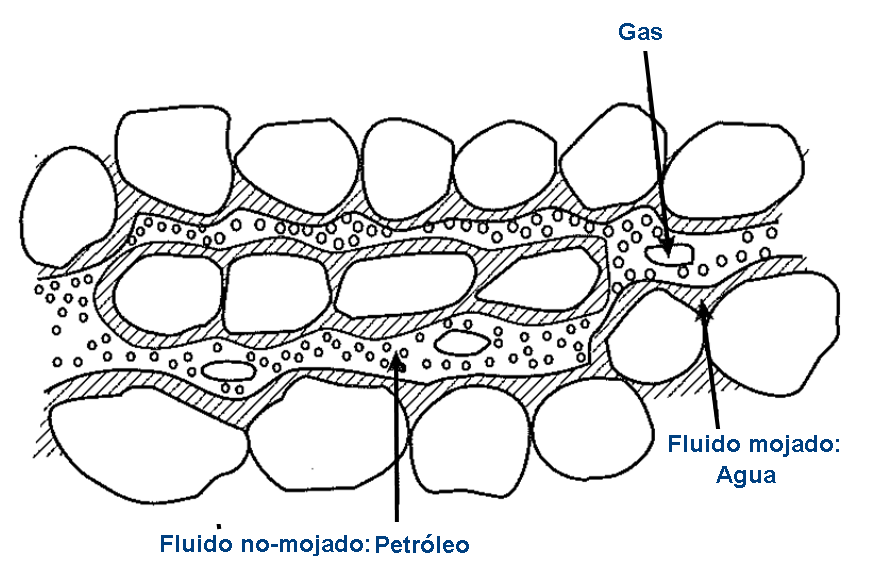
\includegraphics[width=8cm]{Imagenes/Mojabilidad.png}
\caption[Distribución de los fluidos mojado y no-mojado]{Distribución de los fluidos mojado y no-mojado. Modificado de Rosa et al.(2006) \cite{Rosa2006EngenhariaPetroleo}}
\label{fig:fig35}
\end{figure}
%/////////////////////////////////////////////////////////////////////////////////////////
\newpage

%........................................................................................
% TITULO DE LA SUBSECCIÓN 3.4.1
\subsection{Discretización en el Espacio}~\hypertarget{sec:sec341}{}
\label{sec:sec341}

Para la discretización en el domino del espacio se utilizó el método de los residuos ponderados, que se puede consultar con más detalle en los libros de Zienkiewicz et al.(2013) \cite{Zienkiewicz2013TheFundamentals}, Rao (2011) \cite{Rao2011TheEngineering} o Fish et al.(2007) \cite{Fish2007AElements}. Típicamente para la resolución de ecuaciones diferenciales parciales como las que rigen el acoplamiento flujo-geomecánico, se pueden escribir de manera general de la siguiente forma:

%----------------------------------------------------------------------------------------
% ECUACIÓN 3.54
\begin{ceqn} %\label{eq:equ354}
\begin{gather}\label{eq:equ354}
\mathbf{A}\ddot{\Phi} + \mathbf{B}\dot{\Phi} + \mathbf{L}(\Phi) = 0
\end{gather}   
\end{ceqn}
%----------------------------------------------------------------------------------------

donde ($\mathbf{A}$) y ($\mathbf{B}$) son matrices de términos constantes, ($\mathbf{L}$) es un operador diferencial en el espacio de primer orden ($\partial/\partial x$, $\partial/\partial y$ o $\partial/\partial z$) o de segundo orden ($\partial^2/\partial x^2$, $\partial^2/\partial y^2$ o $\partial^2/\partial z^2$) y donde,

%----------------------------------------------------------------------------------------
% ECUACIÓN 3.55
\begin{ceqn} 
\begin{subequations} \label{eq:equ355} 
\begin{gather}
\dot{\Phi}  = \frac{\partial \Phi}{\partial t} \label{eq:equ355a}\\[12pt]
\ddot{\Phi}  = \frac{\partial^2 \Phi}{\partial t^2}  \label{eq:equ355b}
\end{gather}  
\end{subequations} 
\end{ceqn}
%----------------------------------------------------------------------------------------

son las derivadas parciales con respecto al tiempo de primer grado y segundo grado. El termino ($\Phi$) se refiere al vector de incógnitas transitorias que se quieren encontrar, que para esta investigación es el campo de desplazamientos y la presión de poro. Estas incógnitas, son 'discretizadas' o aproximadas por un conjunto finito de parámetros ($\overline{\Phi}$) y funciones de forma ($N$) que se especifican en todo el dominio ($\Omega$), de la siguiente forma:

%----------------------------------------------------------------------------------------
% ECUACIÓN 3.56
\begin{ceqn} %\label{eq:equ356}
\begin{gather}\label{eq:equ356}
\Phi \cong \Phi^h = \displaystyle\sum_{k=1}^{n} N_k\overline{\Phi}_k
\end{gather}   
\end{ceqn}
%----------------------------------------------------------------------------------------


Reemplazando el valor de la función aproximada ($\Phi^h$) en la \textbf{Ecuación} \textbf{\ref{eq:equ354}} obtenemos un residuo que no es igual a cero, pero para el cual
podemos escribir un conjunto de ecuaciones residuales ponderadas de la forma:

%----------------------------------------------------------------------------------------
% ECUACIÓN 3.57
\begin{ceqn} %\label{eq:equ357}
\begin{gather}\label{eq:equ357}
\int\limits_\Omega \mathbf{W}_j\left(\mathbf{A}\ddot{\Phi}^h + \mathbf{B}\dot{\Phi}^h + \mathbf{L}(\Phi^h)\right)\mathbf{d\Omega} = 0
\end{gather}   
\end{ceqn}
%----------------------------------------------------------------------------------------

donde ($\mathbf{W}$) es una función de ponderación arbitraria, cuyo principal requisito es que anule en el contorno. Una opción muy adecuada para la función de ponderación es asumirla igual a las funciones de forma ($N_j$). Esta es la adopción básica adoptada en el método de Galerkin, pero que no hace parte en este estudio. El dominio y contorno adoptado en este estudio se representa en la \textbf{Figura} \textbf{\ref{fig:fig36}}.\bigskip


Después de la integración, la \textbf{Ecuación} \textbf{\ref{eq:equ357}} queda reducida a una ecuación diferencial ordinaria:

%----------------------------------------------------------------------------------------
% ECUACIÓN 3.58
\begin{ceqn} %\label{eq:equ358}
\begin{gather}\label{eq:equ358}
\mathbf{M}\ddot{\overline{\Phi}} + \mathbf{C}\dot{\overline{\Phi}} + \mathbf{P}(\overline{\Phi}) = 0
\end{gather}   
\end{ceqn}
%----------------------------------------------------------------------------------------

donde ($\mathbf{M}$), ($\mathbf{C}$) y ($\mathbf{P}$) son matrices o vectores cuya dimensión corresponde a la dimensión del conjunto total de variables numéricas ($\overline{\Phi}_k$). Por lo general, los parámetros ($\overline{\Phi}$) representan los valores de ($\Phi^h$) en puntos llamados nodos y las funciones de forma, que generalmente son polinomios, describen la interpolación dentro de cada elemento finito, que divide el dominio ($\Omega$). A continuación, se discretizará en el espacio las ecuaciones geomecánicas y de flujo determinadas en el modelo matemático de la sección anterior tanto para medios porosos saturados como parcialmente saturados. En la~\MYhref[blue]{sec:sec343}{Sección 3.4.3} se hará la discretización en el tiempo del modelo geomecánico acoplado.\bigskip


%////////////////////////////////////////////////////////////////////////////////////////
% Figura 3.6

\begin{figure}[!ht]
\centering
\begin{subfigure}[b]{.45\textwidth}
        \centering
        \includegraphics[width=7cm]{Imagenes/Kap_03/Dominio_Real.png}
        \caption{}
        \label{fig:fig36a}
\end{subfigure}
\hfill
\begin{subfigure}[b]{.45\textwidth}
        \centering
        \includegraphics[width=7cm]{Imagenes/Kap_03/Dominio_FEM.png}
        \caption{}
        \label{fig:fig36b}
\end{subfigure}
\captionsetup{format=plain}
\caption[Dominio y contorno del modelo numérico]{Dominio y contorno del modelo numérico. (\subref{fig:fig36a}) Dominio y contorno real; (\subref{fig:fig36b}) Dominio y contorno discretizado.} 
%\vspace*{1cm}
\label{fig:fig36}
\end{figure}
%////////////////////////////////////////////////////////////////////////////////////////



%........................................................................................
% TITULO DE LA SUBSECCIÓN 3.4.1.1
\subsubsection{Medio Poroso Saturado}~\hypertarget{sec:sec3411}{}
\label{sec:sec3411}

El primer paso en la metodología es establecer la forma "\textit{Strong}" del modelo matemático. Esta forma se refiere a la EDP que define el comportamiento del fenómeno físico con sus condiciones de contorno. 

\vspace{0.7cm}
\textbf{A. Forma "\textit{Strong}" del Modelo Geomecánico}\\
Un medio poroso saturado elastoplástico y anisotrópico, su forma "\textit{Strong}" del modelo geomecánico es la siguiente:

%----------------------------------------------------------------------------------------
% ECUACIÓN 3.59
\hfsetfillcolor{gray!50}
\hfsetbordercolor{black}
\begin{ceqn}
\begin{subequations}\label{eq:equ359}
\tikzmarkin{equ352}(4.25,-0.4)(-0.1,-0.4)
\begin{gather}
%\begin{align}
\shortintertext{\textbf{   Forma "\textit{Strong}"}: Medio Poroso Saturado - Modelo Geomecánico}
\normalsize{\mathbf{S}^T\{\mathbf{\sigma}\} + \{\mathbf{b}\} = \{\mathbf{0}\}}
\label{eq:equ359a} %\\[4pt]
\shortintertext{   Condiciones de Contorno} 	
u = \overline{u}\ \text{en}\ \Gamma_u \text{;}\quad \mathbf{\sigma}\cdot\mathbf{\vec{n}} = \mathbf{\overline{t}}\ \text{en}\ \Gamma_t \text{;}\quad \Gamma = \Gamma_u \cup \Gamma_t \label{eq:equ359b} %\\[4pt]
\shortintertext{   donde:}
\normalsize{\{\mathbf{\sigma}\} = [\mathbf{D}]\mathbf{S}\{\mathbf{u}\} - \alpha\{\mathbf{I}\}^T p} \label{eq:equ359c}
\tikzmarkend{equ352}
%\end{align}
\end{gather}
\end{subequations}
\end{ceqn}
%\bigskip
%----------------------------------------------------------------------------------------

\bigskip
\textbf{B. Forma "\textit{Weak}" del Modelo Geomecánico}\\
El siguiente paso es encontrar la forma "\textit{Weak}" de la \textbf{Ecuación} \textbf{\ref{eq:equ359}}. Para eso se debe pre-multiplicar esta ecuación por una función arbitraria ($\mathbf{w}$), cuyo principal requisito es que se desvanezca en el contorno ($\Gamma_{u}$). Luego se integra en todo el dominio ($\Omega$) y se iguala a cero. Estas operaciones en 2-Dimensiones resultan en:


%----------------------------------------------------------------------------------------
% ECUACIÓN 3.60
\begin{ceqn} %\label{eq:equ360}
\begin{gather}\label{eq:equ360}
\iint \limits_\Omega \{\mathbf{w}\}^T \left(\mathbf{S}^T\{\mathbf{\sigma}\} + \{\mathbf{b}\}\right)\mathbf{dV} = \{\mathbf{0}\}
\end{gather}   
\end{ceqn}
%----------------------------------------------------------------------------------------
\\
Reordenando se obtiene:

%----------------------------------------------------------------------------------------
% ECUACIÓN 3.61
\begin{ceqn} %\label{eq:equ361}
\begin{gather}\label{eq:equ361}
\iint \limits_\Omega \{\mathbf{w}\}^T \mathbf{S}^T\{\mathbf{\sigma}\} \mathbf{dV}+ 
\iint \limits_\Omega \{\mathbf{w}\}^T \{\mathbf{b}\} \mathbf{dV} = \{\mathbf{0}\}
\end{gather}   
\end{ceqn}
%----------------------------------------------------------------------------------------
\bigskip
Se debe integrar por partes el primer término de la  \textbf{Ecuación} \textbf{\ref{eq:equ361}}, con ayuda de la fórmula de Green. Para cualquier campo escalar ($\mathbf{r}(x,y)$) y cualquier vector escalar ($\mathbf{s}(x,y)$) se define la ecuación de Green como:

%----------------------------------------------------------------------------------------
% ECUACIÓN 3.62
\begin{ceqn} %\label{eq:equ362}
\begin{gather}\label{eq:equ362}
\iint \limits_\Omega [\mathbf{r}](\nabla \cdot \{\mathbf{s}\})\ dV = 
\oint \limits_\Gamma [\mathbf{r}](\{\mathbf{s}\} \cdot \mathbf{\vec{n}})\ dS -
\iint \limits_\Omega (\nabla [\mathbf{r}]) \cdot \{\mathbf{s}\}\ dV
\end{gather}   
\end{ceqn}
%----------------------------------------------------------------------------------------

\bigskip
Aplicando esta fórmula al primer término de la \textbf{Ecuación} \textbf{\ref{eq:equ361}} se obtiene:

%----------------------------------------------------------------------------------------
% ECUACIÓN 3.63
\begin{ceqn} %\label{eq:equ363}
\begin{gather}\label{eq:equ363}
\iint \limits_\Omega \{\mathbf{w}\}^T \mathbf{S}^T\{\mathbf{\sigma}\} \mathbf{dV} = 
\int \limits_\Gamma \{\mathbf{w}\}^T(\{\mathbf{\sigma}\} \cdot \mathbf{\vec{n}})\ dS -
\iint \limits_\Omega (\{\mathbf{w}\}^T \mathbf{S}^T) \cdot \{\mathbf{\sigma}\}\ dV
\end{gather}   
\end{ceqn}
%----------------------------------------------------------------------------------------

\bigskip
La integral evaluada en el dominio ($\Gamma$) de la \textbf{Ecuación} \textbf{\ref{eq:equ363}} se puede desglosar en el contorno ($\Gamma_{u}$) y el contorno ($\Gamma_{t}$):

%----------------------------------------------------------------------------------------
% ECUACIÓN 3.64
\begin{ceqn} %\label{eq:equ364}
\begin{gather}\label{eq:equ364}
\int \limits_\Gamma \{\mathbf{w}\}^T(\{\mathbf{\sigma}\} \cdot \mathbf{\vec{n}})\ dS =
\int \limits_{\Gamma_{u}} \{\mathbf{w}\}^T(\{\mathbf{\sigma}\} \cdot \mathbf{\vec{n}})\ dS +
\int \limits_{\Gamma_{t}} \{\mathbf{w}\}^T(\{\mathbf{\sigma}\} \cdot \mathbf{\vec{n}})\ dS
\end{gather}   
\end{ceqn}
%----------------------------------------------------------------------------------------

como $\{\mathbf{w}\} = 0$ en $\Gamma_{u}$ y $\{\mathbf{\sigma}\}\cdot \mathbf{\vec{n}} = \{\overline{t}\}$ en $\Gamma_{u}$

%----------------------------------------------------------------------------------------
% ECUACIÓN 3.65
\begin{ceqn} %\label{eq:equ365}
\begin{gather}\label{eq:equ365}
\int \limits_\Gamma \{\mathbf{w}\}^T(\{\mathbf{\sigma}\} \cdot \mathbf{\vec{n}})\ dS =
\int \limits_{\Gamma_{t}} \{\mathbf{w}\}^T \{\overline{t}\}\ dS
\end{gather}   
\end{ceqn}
%----------------------------------------------------------------------------------------

\bigskip
Si descomponemos el lado derecho de la \textbf{Ecuación} \textbf{\ref{eq:equ365}} en sus componentes en 2-Dimensiones se obtiene:

%----------------------------------------------------------------------------------------
% ECUACIÓN 3.66
\begin{ceqn} %\label{eq:equ366}
\begin{gather}\label{eq:equ366}
\int \limits_{\Gamma_{t}} \{\mathbf{w}\}^T \overline{t}\ dS = 
\int \limits_{\Gamma_{tx}} \{\mathbf{w}\}^T \{t_x\}\ dS +
\int \limits_{\Gamma_{ty}} \{\mathbf{w}\}^T \{t_y\}\ dS
\end{gather}   
\end{ceqn}
%----------------------------------------------------------------------------------------

donde 

%----------------------------------------------------------------------------------------
% ECUACIÓN 3.67
\begin{ceqn} %\label{eq:equ367}
\begin{gather}\label{eq:equ367}
\{t_x\} = \begin{Bmatrix} \overline{t}_x \\ 0 \end{Bmatrix}\ \text{;}\quad
\{t_y\} = \begin{Bmatrix} 0 \\ \overline{t}_y \end{Bmatrix}\
\end{gather}   
\end{ceqn}
%----------------------------------------------------------------------------------------

\bigskip
Por lo tanto, la \textbf{Ecuación} \textbf{\ref{eq:equ363}} se convierte en:

%----------------------------------------------------------------------------------------
% ECUACIÓN 3.68
\begin{ceqn} %\label{eq:equ368}
\begin{gather}\label{eq:equ368}
\iint \limits_\Omega \{\mathbf{w}\}^T \mathbf{S}^T\{\mathbf{\sigma}\} \mathbf{dV} = 
\int \limits_{\Gamma_{tx}} \{\mathbf{w}\}^T \{t_x\}\ dS +
\int \limits_{\Gamma_{ty}} \{\mathbf{w}\}^T \{t_y\}\ dS -
\iint \limits_\Omega (\{\mathbf{w}\}^T \mathbf{S}^T) \cdot \{\mathbf{\sigma}\}\ dV
\end{gather}   
\end{ceqn}
%----------------------------------------------------------------------------------------

\bigskip
Reemplazando la \textbf{Ecuación} \textbf{\ref{eq:equ368}} en la \textbf{Ecuación} \textbf{\ref{eq:equ361}} se obtiene la forma "\textit{Weak}" del modelo geomecánico para un medio poroso saturado:

%----------------------------------------------------------------------------------------
% ECUACIÓN 3.69
\hfsetfillcolor{gray!50}
\hfsetbordercolor{black}
\begin{ceqn}
\begin{subequations}\label{eq:equ369}
\tikzmarkin{equ369}(5.25,-0.4)(-0.1,-0.4)
\begin{gather}
%\begin{align}
\shortintertext{\textbf{   Forma "\textit{Weak}"}: Medio Poroso Saturado - Modelo Geomecánico}
\iint \limits_\Omega (\{\mathbf{w}\}^T \mathbf{S}^T) \cdot \{\mathbf{\sigma}\}\ dV = 
\iint \limits_\Omega \{\mathbf{w}\}^T \{\mathbf{b}\} \mathbf{dV} +
\int \limits_{\Gamma_{tx}} \{\mathbf{w}\}^T \{t_x\}\ dS +
\int \limits_{\Gamma_{ty}} \{\mathbf{w}\}^T \{t_y\}\ dS 
\label{eq:equ369a} %\\[4pt]
\shortintertext{   Condiciones de Contorno} 	
u = \overline{u}\ \text{en}\ \Gamma_u \text{;}\quad \mathbf{\sigma_x}\cdot\mathbf{\vec{n}} = \mathbf{\overline{t}_x}\ \text{en}\ \Gamma_{tx} \text{;}\quad 
\mathbf{\sigma_y}\cdot\mathbf{\vec{n}} = \mathbf{\overline{t}_y}\ \text{en}\ \Gamma_{ty} \text{;}\quad
\Gamma = \Gamma_u \cup \Gamma_t \label{eq:equ369b} %\\[4pt]
\shortintertext{   donde:}
\normalsize{\{\mathbf{\sigma}\} = [\mathbf{D}]\mathbf{S}\{\mathbf{u}\} - \alpha\{\mathbf{I}\}^T p} \label{eq:equ369c}\\[4pt]
\normalsize{\{\mathbf{w}\} = 0\quad \text{en}\quad \Gamma_{u}} \label{eq:equ362d}
\tikzmarkend{equ369}
%\end{align}
\end{gather}
\end{subequations}
\end{ceqn}
%\bigskip
%----------------------------------------------------------------------------------------


\bigskip\bigskip
\textbf{C. Discretización en el Espacio del Modelo Geomecánico}\\
Para realizar la discretización de la forma "\textit{Weak}" del modelo geomecánico se deben plantear las siguientes definiciones:


%----------------------------------------------------------------------------------------
% ECUACIÓN 3.70
\begin{ceqn} 
\begin{subequations} \label{eq:equ370} 
\begin{gather}
\{\mathbf{u}^e\} \cong  \left[\mathbf{N_u}\right] \{\mathbf{U}^e\} \label{eq:equ370a}\\[10pt]
\mathbf{p}^e \cong  \left[\mathbf{N_p}\right] \mathbf{P}^e \label{eq:equ370b}\\[10pt]
\{\mathbf{w}^e\} \cong \{\mathbf{w_u}^e\} = \left[\mathbf{N_u}\right] \{\mathbf{W_u}^e\}\ \label{eq:equ370c}\\[10pt]
\{\mathbf{w}^e\} \cong \{\mathbf{w_p}^e\} = \left[\mathbf{N_p}\right] \{\mathbf{W_p}^e\}\ \label{eq:equ370d}
\end{gather}  
\end{subequations} 
\end{ceqn}
%----------------------------------------------------------------------------------------

\bigskip
donde ($\mathbf{u}^e$) es el campo vectorial de desplazamientos, ($\mathbf{N_u}$) es la matriz de funciones de forma de los desplazamientos, ($\mathbf{U}^e$) es el vector de valores nodales de desplazamientos, ($\mathbf{p}^e$) es el campo escalar de presiones de poros, ($\mathbf{N_p}$) es la matriz de funciones de forma de las presiones de poros, ($\mathbf{P}^e$) son los valores nodales de la presión, ($\mathbf{w_u}^e$) es el vector de funciones de ponderación y ($\mathbf{W_u}^e$) es el vector de valores nodales de la función de ponderación. Todas estas magnitudes tienen el superíndice ($e$) que significa que son evaluados en un solo elemento finito. Por lo tanto, se evalúan estos valores en cada elemento finito del dominio discretizado y luego se suman todas las contribuciones de cada elemento en un solo esquema global.\bigskip

El siguiente paso es reemplazar las expresiones de la \textbf{Ecuación} \textbf{\ref{eq:equ370}} en la \textbf{Ecuación} \textbf{\ref{eq:equ369}} y con esto se evalúa la contribución que hace al problema un solo elemento finito. Pero antes de hacer esto se debe escribir de la manera siguiente la \textbf{Ecuación} \textbf{\ref{eq:equ369}}:\bigskip

%----------------------------------------------------------------------------------------
% ECUACIÓN 3.71
\begin{ceqn} 
%\begin{subequations}  
\begin{gather}\label{eq:equ371}
\begin{multlined}
\iint \limits_{\Omega^e} \{\mathbf{w}^e\}^T \mathbf{S}^T[\mathbf{D}^e]\mathbf{S}\{\mathbf{u}^e\}\ dV = 
\iint \limits_{\Omega^e} \{\mathbf{w_u}^e\}^T \alpha \nabla p^e\ dV +
\iint \limits_{\Omega^e} \{\mathbf{w_u}^e\}^T \{\mathbf{b}^e\}\ dV\ +\\[10pt]
\int \limits_{\Gamma^e_{tx}} \{\mathbf{w_u}^e\}^T \{t^e_x\}\ dS\ +
\int \limits_{\Gamma^e_{ty}} \{\mathbf{w_u}^e\}^T \{t^e_y\}\ dS
%\label{eq:equ346a}
\end{multlined}
\end{gather}  
%\end{subequations} 
\end{ceqn}
%----------------------------------------------------------------------------------------

Reemplazando la \textbf{Ecuación} \textbf{\ref{eq:equ370}} en cada miembro de la \textbf{Ecuación} \textbf{\ref{eq:equ371}} resulta en una ecuación que evalúa el aporte de un elemento finito cualquiera en todo el esquema global. Por ejemplo, para el lado izquierdo de la \textbf{Ecuación} \textbf{\ref{eq:equ362}} resulta en:\bigskip


%----------------------------------------------------------------------------------------
% ECUACIÓN 3.72
\begin{ceqn} %\label{eq:equ372}
\begin{gather}\label{eq:equ372}
\iint \limits_{\Omega^e} \{\mathbf{w}^e\}^T \mathbf{S}^T[\mathbf{D}^e]\mathbf{S}\{\mathbf{u}^e\}\ dV = 
\iint \limits_{\Omega^e} \{\mathbf{W_u}^e\}^T \{\mathbf{N_u}^e\}^T \mathbf{S}^T  [\mathbf{D}^e] \{\mathbf{W_u}^e\} \mathbf{S} \{\mathbf{N_u}^e\} \{\mathbf{U}^e\}\ dV
\end{gather}   
\end{ceqn}
%----------------------------------------------------------------------------------------
\\
Definiendo para el modelo geomecánico:

%----------------------------------------------------------------------------------------
% ECUACIÓN 3.73
\begin{ceqn} 
\begin{subequations} \label{eq:equ373} 
\begin{gather}
[\mathbf{B_u}^e] = \mathbf{S} \{\mathbf{N_u}^e\} \label{eq:equ373a}\\[10pt]
[\mathbf{B_u}^e]^T = \{\mathbf{N_u}^e\}^T \mathbf{S}^T  \label{eq:equ373b}\\[10pt]
\mathbf{P}^e =  \left[\mathbf{L^e}\right] \mathbf{P} \label{eq:equ373c}\\[10pt]
\{\mathbf{W_u}^e\} = \left[\mathbf{L^e}\right] \{\mathbf{W_u}\}  \label{eq:equ373d}\\[10pt]
\{\mathbf{W_u}^e\}^T = \{\mathbf{W_u}\}^T \left[\mathbf{L^e}\right]^T  \label{eq:equ373e}
\end{gather}  
\end{subequations} 
\end{ceqn}
%----------------------------------------------------------------------------------------
\\
Reemplazando la \textbf{Ecuación} \textbf{\ref{eq:equ373}} en cada miembro de la \textbf{Ecuación} \textbf{\ref{eq:equ372}} resulta en:

%----------------------------------------------------------------------------------------
% ECUACIÓN 3.74
\begin{ceqn} %\label{eq:equ374}
\begin{gather}\label{eq:equ374}
\iint \limits_{\Omega^e} \{\mathbf{w}^e\}^T \mathbf{S}^T[\mathbf{D}^e]\mathbf{S}\{\mathbf{u}^e\}\ dV = 
\{\mathbf{W_u}\}^T \left[\mathbf{L}^e\right]^T \left( \iint \limits_{\Omega^e}  [\mathbf{B_u}^e]^T [\mathbf{D}^e] [\mathbf{B_u}^e]\ dV \right) \left[\mathbf{L}^e\right] \{\mathbf{U}\}
\end{gather}   
\end{ceqn}
%----------------------------------------------------------------------------------------
\\
donde ($\mathbf{B}^e$) es la matriz de deformación-desplazamiento, ($\mathbf{L}^e$) es la matriz de ensamblaje del elemento, ($U$) es el campo de deformaciones de todo el dominio del problema, ($\mathbf{W}$) es la matriz de ponderación de todo el dominio del problema.\bigskip 

La función de la matriz ($\mathbf{L}^e$) es ensamblar la contribución que realiza cada elemento en el esquema global del problema. Realizando este mismo procedimiento para el resto de miembros de la  \textbf{Ecuación} \textbf{\ref{eq:equ371}} se obtiene:

%----------------------------------------------------------------------------------------
% ECUACIÓN 3.75
\begin{ceqn} %\label{eq:equ375}
\begin{gather}\label{eq:equ375}
\iint \limits_{\Omega^e} \{\mathbf{w}^e\}^T \alpha \nabla p^e\ dV = 
\{\mathbf{W_u}\}^T \left[\mathbf{L}^e\right]^T \left( \iint \limits_{\Omega^e}  [\mathbf{N_u}^e]^T \alpha \nabla [\mathbf{N_p}^e]\ dV \right) \left[\mathbf{L}^e\right] \{\mathbf{P}\}
\end{gather}   
\end{ceqn}
%----------------------------------------------------------------------------------------

%----------------------------------------------------------------------------------------
% ECUACIÓN 3.76
\begin{ceqn} %\label{eq:equ376}
\begin{gather}\label{eq:equ376}
\iint \limits_{\Omega^e} \{\mathbf{w}^e\}^T \{\mathbf{b}^e\}\ dV\ = 
\{\mathbf{W_u}\}^T \left[\mathbf{L}^e\right]^T \left( \iint \limits_{\Omega^e}  [\mathbf{N_u}^e]^T  \{\mathbf{b}^e\}\ dV \right) \left[\mathbf{L}^e\right]
\end{gather}   
\end{ceqn}
%----------------------------------------------------------------------------------------

%----------------------------------------------------------------------------------------
% ECUACIÓN 3.77
\begin{ceqn} %\label{eq:equ377}
\begin{gather}\label{eq:equ377}
\int \limits_{\Gamma^e_{tx}} \{\mathbf{w}^e\}^T \{t^e_x\}\ dS\ = 
\{\mathbf{W_u}\}^T \left[\mathbf{L}^e\right]^T \left( \int \limits_{\Gamma^e_{tx}} [\mathbf{N_u}^e]^T  \{t^e_x\}\ dV \right) \left[\mathbf{L}^e\right]
\end{gather}   
\end{ceqn}
%----------------------------------------------------------------------------------------

%----------------------------------------------------------------------------------------
% ECUACIÓN 3.78
\begin{ceqn} %\label{eq:equ378}
\begin{gather}\label{eq:equ378}
\int \limits_{\Gamma^e_{ty}} \{\mathbf{w}^e\}^T \{t^e_y\}\ dS\ = 
\{\mathbf{W_u}\}^T \left[\mathbf{L}^e\right]^T \left( \int \limits_{\Gamma^e_{ty}} [\mathbf{N_u}^e]^T  \{t^e_y\}\ dV \right) \left[\mathbf{L}^e\right]
\end{gather}   
\end{ceqn}
%----------------------------------------------------------------------------------------

\bigskip
Uniendo las \textbf{Ecuaciones} \textbf{\ref{eq:equ374}}, \textbf{\ref{eq:equ375}}, \textbf{\ref{eq:equ376}}, \textbf{\ref{eq:equ377}} y \textbf{\ref{eq:equ378}} y sumando todas las contribuciones de los elementos se obtiene una ecuación general:

%----------------------------------------------------------------------------------------
% ECUACIÓN 3.79
\begin{ceqn} 
\begin{gather}\label{eq:equ379}
\begin{multlined}
 \{\mathbf{W_u}\}^T  \displaystyle\sum_{e=1}^{N_e} \left[ \left[\mathbf{L}^e\right]^T \left( \iint \limits_{\Omega^e}  [\mathbf{B}^e]^T [\mathbf{D}^e] [\mathbf{B}^e]\ dV \right) \left[\mathbf{L}^e\right] \right] \{\mathbf{U}\}\\[10pt]
-\ \{\mathbf{W_u}\}^T \displaystyle\sum_{e=1}^{N_e} \left[ \left[\mathbf{L}^e\right]^T \left( \iint \limits_{\Omega^e}  [\mathbf{N_u}^e]^T \alpha \nabla [\mathbf{N_p}^e]\ dV \right) \left[\mathbf{L}^e\right] \right] \{\mathbf{P}\} \\[10pt]
-\ \{\mathbf{W_u}\}^T \displaystyle\sum_{e=1}^{N_e} \left[ \left[\mathbf{L}^e\right]^T \left( \iint \limits_{\Omega^e}  [\mathbf{N_u}^e]^T  \{\mathbf{b}^e\}\ dV \right) \left[\mathbf{L}^e\right] \right] \\[10pt]
-\ \{\mathbf{W_u}\}^T \displaystyle\sum_{e=1}^{N_e} \left[ \left[\mathbf{L}^e\right]^T \left( \int \limits_{\Gamma^e_{tx}} [\mathbf{N_u}^e]^T  \{t^e_x\}\ dV \right) \left[\mathbf{L}^e\right] \right] \\[10pt]
-\ \{\mathbf{W_u}\}^T \displaystyle\sum_{e=1}^{N_e} \left[ \left[\mathbf{L}^e\right]^T \left( \int \limits_{\Gamma^e_{ty}} [\mathbf{N_u}^e]^T  \{t^e_y\}\ dV \right) \left[\mathbf{L}^e\right] \right]  = 0 \\[10pt]
\end{multlined}
\end{gather}  
\end{ceqn}
%----------------------------------------------------------------------------------------

Como $\{\mathbf{W_u}\}^T$ es factor común de todos los términos de la \textbf{Ecuación} \textbf{\ref{eq:equ379}} se puede descartar y por tanto, queda discretizada la forma "\textit{Weak}" del modelo geomecánico para un suelo saturado.
\newpage


%----------------------------------------------------------------------------------------
% ECUACIÓN 3.80
\hfsetfillcolor{gray!50}
\hfsetbordercolor{black}
\begin{ceqn}
\begin{subequations}\label{eq:equ373}
\tikzmarkin{equ380}(0.95,-0.4)(-0.1,-0.4)
\begin{gather}
%\begin{align}
\shortintertext{\textbf{   Forma Discretizada}: Medio Poroso Saturado - Modelo Geomecánico}
[\mathbf{M}]\{\mathbf{U}\} - [\mathbf{C}]\{\mathbf{P}\} = \{\mathbf{f_u}\}
\label{eq:equ380a} %\\[4pt]
\shortintertext{   donde:}
[\mathbf{M}] = \displaystyle\sum_{e=1}^{N_e} [\mathbf{L}^e]^T [\mathbf{M}^e]   [\mathbf{L}^e] \label{eq:equ380b}\\[4pt]
[\mathbf{M}^e] = \iint \limits_{\Omega^e}  [\mathbf{B_u}^e]^T [\mathbf{D}^e] [\mathbf{B_u}^e]\ dV \label{eq:equ380c}\\[4pt]
[\mathbf{C}] = \displaystyle\sum_{e=1}^{N_e} [\mathbf{L}^e]^T [\mathbf{C}^e]   [\mathbf{L}^e] \label{eq:equ380d}\\[4pt]
[\mathbf{C}^e] = \iint \limits_{\Omega^e}  [\mathbf{N_u}^e]^T \alpha \nabla [\mathbf{N_p}^e]\ dV \label{eq:equ380e}\\[4pt]
\{\mathbf{f_u}\} = \displaystyle\sum_{e=1}^{N_e} [\mathbf{L}^e]^T \{\mathbf{f_u}^e\} \label{eq:equ380f}\\[4pt]
\{\mathbf{f_u}^e\} = \iint \limits_{\Omega^e}  [\mathbf{N_u}^e]^T  \{\mathbf{b}^e\}\ dV +
\int \limits_{\Gamma^e_{tx}} [\mathbf{N_u}^e]^T  \{t^e_x\}\ dV + \int \limits_{\Gamma^e_{ty}} [\mathbf{N_u}^e]^T  \{t^e_y\}\ dV
\label{eq:equ380g}\\[4pt]
\shortintertext{   Condiciones de Contorno} 	
u = \overline{u}\ \text{en}\ \Gamma_u \text{;}\quad \mathbf{\sigma_x}\cdot\mathbf{\vec{n}} = \mathbf{\overline{t}_x}\ \text{en}\ \Gamma_{tx} \text{;}\quad 
\mathbf{\sigma_y}\cdot\mathbf{\vec{n}} = \mathbf{\overline{t}_y}\ \text{en}\ \Gamma_{ty} \text{;}\quad
\Gamma = \Gamma_u \cup \Gamma_t \label{eq:equ380h} %\\[4pt]
\tikzmarkend{equ380}
%\end{align}
\end{gather}
\end{subequations}
\end{ceqn}
%\bigskip
%----------------------------------------------------------------------------------------

\vspace{1cm}
\textbf{D. Forma "\textit{Strong}" del Modelo de Flujo}\\
 Para el modelo de flujo de un medio poroso saturado se utilizó el mismo procedimiento que se utilizó en el modelo geomecánico. Por lo tanto, para un medio poroso saturado con características elastoplásticas y anisotrópicas la forma "\textit{Strong}" del modelo de flujo es la siguiente:

%----------------------------------------------------------------------------------------
% ECUACIÓN 3.81
\hfsetfillcolor{gray!50}
\hfsetbordercolor{black}
\begin{ceqn}
\begin{subequations}\label{eq:equ381}
\tikzmarkin{equ381}(3.5,-0.5)(-0.1,-0.5)
\begin{gather}
%\begin{align}
\shortintertext{\textbf{   Forma "\textit{Strong}"}: Medio Poroso Saturado - Modelo de Flujo}
\nabla^T \left[\frac{[\mathbf{K}]}{\mu}\nabla p\right] = \alpha \nabla^T \{\mathbf{\dot{u}}\} + \frac{1}{Q} \dot{p}
\label{eq:equ381a} \\[8pt]
\shortintertext{   Condiciones de Contorno} 	
p = \overline{p}\ \text{en}\ \Gamma_p \text{;}\quad \nabla p \cdot\mathbf{\vec{n}} = \mathbf{\overline{q}}\ \text{en}\ \Gamma_q \text{;}\quad \Gamma = \Gamma_p \cup \Gamma_q \label{eq:equ381b} %\\[4pt]
\shortintertext{   donde:}
\frac{1}{Q} = \frac{\phi}{K_f} + \frac{(1-\phi)}{K_m}-\frac{\{\mathbf{I}\}[\mathbf{D}]\{\mathbf{I}\}^T}{(3K_{m})^{2}} \label{eq:equ381c}
\tikzmarkend{equ381}
%\end{align}
\end{gather}
\end{subequations}
\end{ceqn}
%\bigskip
%----------------------------------------------------------------------------------------
%\\


\textbf{E. Forma "\textit{Weak}" del Modelo de Flujo}\\
El siguiente paso es encontrar la forma "\textit{Weak}" de la \textbf{Ecuación} \textbf{\ref{eq:equ381}}. Pre-multiplicando esta ecuación por $\{\mathbf{w}\}^T$ y reordenando se obtiene:\bigskip

%----------------------------------------------------------------------------------------
% ECUACIÓN 3.82
\begin{ceqn} %\label{eq:equ382}
\begin{gather}\label{eq:equ382}
\iint \limits_\Omega \{\mathbf{w_p}\}^T \nabla^T \left[\frac{[\mathbf{K}]}{\mu}\nabla p\right] dV - 
\iint \limits_\Omega \{\mathbf{w_p}\}^T \alpha \nabla^T \{\mathbf{\dot{u}}\}\ dV -
\iint \limits_\Omega \{\mathbf{w_p}\}^T \frac{1}{Q} \dot{p} dV = \{\mathbf{0}\}
\end{gather}   
\end{ceqn}
%----------------------------------------------------------------------------------------

\bigskip
Aplicando la fórmula de Green en el primer término de la \textbf{Ecuación} \textbf{\ref{eq:equ382}} y aplicando las condiciones de contorno respectivas se obtiene:

%----------------------------------------------------------------------------------------
% ECUACIÓN 3.83
\begin{ceqn} %\label{eq:equ383}
\begin{gather}\label{eq:equ383}
\iint \limits_\Omega \{\mathbf{w_p}\}^T \nabla^T \left[\frac{[\mathbf{K}]}{\mu}\nabla p\right] dV = 
\int \limits_{\Gamma_{q}} \{\mathbf{w_p}\}^T q\ dS -
\iint \limits_\Omega \{\mathbf{w_p}\}^T \nabla^T \cdot \frac{[\mathbf{K}]}{\mu}\nabla p\ dV
\end{gather}   
\end{ceqn}
%----------------------------------------------------------------------------------------

\bigskip
Reemplazando la \textbf{Ecuación} \textbf{\ref{eq:equ383}} en la \textbf{Ecuación} \textbf{\ref{eq:equ382}} se obtiene la forma "\textit{Weak}" del modelo de flujo para un medio poroso saturado:

%----------------------------------------------------------------------------------------
% ECUACIÓN 3.84
\hfsetfillcolor{gray!50}
\hfsetbordercolor{black}
\begin{ceqn}
\begin{subequations}\label{eq:equ384}
\tikzmarkin{equ384a}(4.0,-0.5)(-0.1,-0.4)
\begin{gather}
%\begin{align}
\shortintertext{\textbf{   Forma "\textit{Weak}"}: Medio Poroso Saturado - Modelo de Flujo}
\iint \limits_\Omega \{\mathbf{w}\}^T \nabla^T \cdot \frac{[\mathbf{K}]}{\mu}\nabla p\ dV = \iint \limits_\Omega \{\mathbf{w}\}^T \frac{1}{Q} \dot{p}\ dV +
\iint \limits_\Omega \{\mathbf{w}\}^T \alpha \nabla^T \{\mathbf{\dot{u}}\}\ dV +
\int \limits_{\Gamma_{q}} \{\mathbf{w}\}^T q\ dS 
\label{eq:equ384a} %\\[4pt]
\shortintertext{   Condiciones de Contorno} 	
p = \overline{p}\ \text{en}\ \Gamma_u \text{;}\quad \nabla p \cdot \mathbf{\vec{n}} = \overline{q}\ \text{en}\ \Gamma_{q} \text{;}\quad
\Gamma = \Gamma_p \cup \Gamma_q \label{eq:equ384b} %\\[4pt]
\shortintertext{   donde:}
\frac{1}{Q} = \frac{\phi}{K_f} + \frac{(1-\phi)}{K_m}-\frac{\{\mathbf{I}\}[\mathbf{D}]\{\mathbf{I}\}^T}{(3K_{m})^{2}} \label{eq:equ384c}
\tikzmarkend{equ384a}
%\end{align}
\end{gather}
\end{subequations}
\end{ceqn}
%\bigskip
%----------------------------------------------------------------------------------------

\bigskip\bigskip
\textbf{F. Discretización en el Espacio del Modelo de Flujo}\\
Para realizar la discretización de la forma "\textit{Weak}" del modelo de flujo se remplazan las expresiones de la \textbf{Ecuación} \textbf{\ref{eq:equ363}} en la \textbf{Ecuación} \textbf{\ref{eq:equ384}} y con esto se evalúa la contribución que hace al problema un solo elemento finito. Pero antes de hacer esto se debe escribir de la manera siguiente la \textbf{Ecuación} \textbf{\ref{eq:equ370}}:\bigskip

%----------------------------------------------------------------------------------------
% ECUACIÓN 3.85
\begin{ceqn} 
%\begin{subequations}  
\begin{gather}\label{eq:equ385}
\begin{multlined}
\iint \limits_{\Omega^e} \{\mathbf{w}^e\}^T \nabla^T \cdot \frac{[\mathbf{K}^e]}{\mu^e}\nabla p^e\ dV + \iint \limits_{\Omega^e} \{\mathbf{w}^e\}^T \frac{1}{Q^e}\ \dot{p^e}\ dV \\[8pt]
+ \iint \limits_{\Omega^e}\{\mathbf{w}^e\}^T \alpha \nabla^T \{\mathbf{\dot{u}}^e\}\ dV -
\int \limits_{\Gamma_{q}^e} \{\mathbf{w}^e\}^T \overline{q}^e\ dS = \{\mathbf{0}\}
%\label{eq:equ346a}
\end{multlined}
\end{gather}  
%\end{subequations} 
\end{ceqn}
%----------------------------------------------------------------------------------------


Reemplazando la \textbf{Ecuación} \textbf{\ref{eq:equ363}} en cada miembro de la \textbf{Ecuación} \textbf{\ref{eq:equ385}} resulta en una ecuación que evalúa el aporte de un elemento finito cualquiera en todo el esquema global. Por ejemplo, para el lado izquierdo de la \textbf{Ecuación} \textbf{\ref{eq:equ385}} resulta en:\bigskip


%----------------------------------------------------------------------------------------
% ECUACIÓN 3.86
\begin{ceqn} %\label{eq:equ386}
\begin{gather}\label{eq:equ386}
\iint \limits_{\Omega^e} \{\mathbf{w}^e\}^T \nabla^T \cdot \frac{[\mathbf{K}^e]}{\mu^e} \nabla p^e\ dV = 
\iint \limits_{\Omega^e} \{\mathbf{W_p}^e\}^T \{\mathbf{N_p}^e\}^T \nabla^T  \frac{[\mathbf{K}^e]}{\mu^e} \{\mathbf{W_p}^e\} \nabla \{\mathbf{N_p}^e\} \{\mathbf{P}^e\}\ dV
\end{gather}   
\end{ceqn}
%----------------------------------------------------------------------------------------

Definiendo para el modelo de flujo:
%\vspace{-0.5cm}
%----------------------------------------------------------------------------------------
% ECUACIÓN 3.87
\begin{ceqn} 
\begin{subequations} \label{eq:equ387} 
\begin{gather}
[\mathbf{B_p}^e] = \nabla \{\mathbf{N_p}^e\} \label{eq:equ387a}\\[10pt]
[\mathbf{B_p}^e]^T = \{\mathbf{N_p}^e\}^T \nabla^T  \label{eq:equ387b}\\[10pt]
\{\mathbf{W_p}^e\}^T = \{\mathbf{W_p}\}^T \left[\mathbf{L^e}\right]^T  \label{eq:equ387c}
\end{gather}  
\end{subequations} 
\end{ceqn}
%----------------------------------------------------------------------------------------

Reemplazando la \textbf{Ecuación} \textbf{\ref{eq:equ387}} en cada miembro de la \textbf{Ecuación} \textbf{\ref{eq:equ385}} resulta en:

%----------------------------------------------------------------------------------------
% ECUACIÓN 3.88
\begin{ceqn} %\label{eq:equ388}
\begin{gather}\label{eq:equ388}
\iint \limits_{\Omega^e} \{\mathbf{w}^e\}^T \nabla^T \cdot \frac{[\mathbf{K}^e]}{\mu^e} \nabla p^e\ dV = 
\{\mathbf{W_p}\}^T \left[\mathbf{L}^e\right]^T \left( \iint \limits_{\Omega^e}  [\mathbf{B_p}^e]^T \frac{[\mathbf{K}^e]}{\mu^e} [\mathbf{B_p}^e]\ dV \right) \left[\mathbf{L}^e\right] \mathbf{P}
\end{gather}   
\end{ceqn}
%----------------------------------------------------------------------------------------

donde ($\mathbf{B_p}^e$) es la matriz de presiones-caudales, ($\mathbf{W_p}$) es la matriz de ponderación de presiones de poros para todo el dominio del problema. Realizando este mismo procedimiento para el resto de miembros de la  \textbf{Ecuación} \textbf{\ref{eq:equ385}} se obtiene:
%\vspace{-0.5cm}
%----------------------------------------------------------------------------------------
% ECUACIÓN 3.89
\begin{ceqn} %\label{eq:equ389}
\begin{gather}\label{eq:equ389}
\iint \limits_{\Omega^e} \{\mathbf{w}^e\}^T \frac{1}{Q^e}\ \dot{p^e} = 
\{\mathbf{W_p}\}^T \left[\mathbf{L}^e\right]^T \left( \iint \limits_{\Omega^e}  [\mathbf{N_p}^e]^T \frac{1}{Q^e}\ [\mathbf{N_p}^e]\ dV \right) \left[\mathbf{L}^e\right] \mathbf{\dot{P}}
\end{gather}   
\end{ceqn}
%----------------------------------------------------------------------------------------

%----------------------------------------------------------------------------------------
% ECUACIÓN 3.90
\begin{ceqn} %\label{eq:equ390}
\begin{gather}\label{eq:equ390}
\iint \limits_{\Omega^e}\{\mathbf{w}^e\}^T \alpha \nabla^T \{\mathbf{\dot{u}}^e\}\ dV\ = 
\{\mathbf{W_p}\}^T \left[\mathbf{L}^e\right]^T \left( \iint \limits_{\Omega^e}  [\mathbf{N_p}^e]^T  \alpha \nabla^T [\mathbf{N_u}^e]\ dV \right) \left[\mathbf{L}^e\right]\{\mathbf{\dot{U}}\}
\end{gather}   
\end{ceqn}
%----------------------------------------------------------------------------------------

%----------------------------------------------------------------------------------------
% ECUACIÓN 3.91
\begin{ceqn} %\label{eq:equ391}
\begin{gather}\label{eq:equ391}
\int \limits_{\Gamma_{q}^e} \{\mathbf{w}^e\}^T q^e\ dS\ = 
\{\mathbf{W_p}\}^T \left[\mathbf{L}^e\right]^T \left( \int \limits_{\Gamma^e_{tx}} [\mathbf{N_p}^e]^T \overline{q}\ dV \right) \left[\mathbf{L}^e\right]
\end{gather}   
\end{ceqn}
%----------------------------------------------------------------------------------------

\vspace{0.5cm}
Uniendo las \textbf{Ecuaciones} \textbf{\ref{eq:equ388}}, \textbf{\ref{eq:equ389}}, \textbf{\ref{eq:equ390}}, y \textbf{\ref{eq:equ391}} y sumando todas las contribuciones de los elementos se obtiene la ecuación general:

%----------------------------------------------------------------------------------------
% ECUACIÓN 3.92
\begin{ceqn} 
\begin{gather}\label{eq:equ392}
\begin{multlined}
 \{\mathbf{W_p}\}^T  \displaystyle\sum_{e=1}^{N_e} \left[ \left[\mathbf{L}^e\right]^T \left( \iint \limits_{\Omega^e}  [\mathbf{B_p}^e]^T \frac{[\mathbf{K}^e]}{\mu^e} [\mathbf{B_p}^e]\ dV \right) \left[\mathbf{L}^e\right] \right] \mathbf{P}\\[10pt]
+\ \{\mathbf{W_p}\}^T \displaystyle\sum_{e=1}^{N_e} \left[ \left[\mathbf{L}^e\right]^T \left( \iint \limits_{\Omega^e}  [\mathbf{N_p}^e]^T \frac{1}{Q^e}\ [\mathbf{N_p}^e]\ dV \right) \left[\mathbf{L}^e\right] \right] \mathbf{\dot{P}} \\[10pt]
+\ \{\mathbf{W_p}\}^T \displaystyle\sum_{e=1}^{N_e} \left[ \left[\mathbf{L}^e\right]^T \left( \iint \limits_{\Omega^e}  [\mathbf{N_p}^e]^T  \alpha \nabla^T [\mathbf{N_u}^e]\ dV \right) \left[\mathbf{L}^e\right] \right]\{\mathbf{\dot{U}}\}  \\[10pt]
-\ \{\mathbf{W_p}\}^T \displaystyle\sum_{e=1}^{N_e} \left[ \left[\mathbf{L}^e\right]^T \left(  \int \limits_{\Gamma^e_{tx}} [\mathbf{N_p}^e]^T \overline{q}\ dV \right) \left[\mathbf{L}^e\right] \right] = \{\mathbf{0}\}
\end{multlined}
\end{gather}  
\end{ceqn}
%----------------------------------------------------------------------------------------

Como $\{\mathbf{W_p}\}^T$ es factor común de todos los términos de la \textbf{Ecuación} \textbf{\ref{eq:equ392}} se puede descartar y por tanto, queda discretizada la forma "\textit{Weak}" del modelo geomecánico para un suelo saturado.


%----------------------------------------------------------------------------------------
% ECUACIÓN 3.93
\hfsetfillcolor{gray!50}
\hfsetbordercolor{black}
\begin{ceqn}
\begin{subequations}\label{eq:equ393}
\tikzmarkin{equ393a}(2.8,-0.5)(-0.1,-0.4)
\begin{gather}
%\begin{align}
\shortintertext{\textbf{   Forma Discretizada}: Medio Poroso Saturado - Modelo de Flujo}
[\mathbf{H}]\mathbf{P} + [\mathbf{S}]\mathbf{\dot{P}} + [\mathbf{C}]^T\{\mathbf{\dot{U}}\} = \{\mathbf{f_p}\}
\label{eq:equ393a} %\\[4pt]
\shortintertext{   donde:}
[\mathbf{H}] = \displaystyle\sum_{e=1}^{N_e} [\mathbf{L}^e]^T [\mathbf{H}^e]   [\mathbf{L}^e] \label{eq:equ393b}\\[4pt]
[\mathbf{H}^e] = \iint \limits_{\Omega^e}  [\mathbf{B_p}^e]^T \frac{[\mathbf{K}^e]}{\mu^e} [\mathbf{B_p}^e]\ dV \label{eq:equ393c}\\[4pt]
[\mathbf{S}] = \displaystyle\sum_{e=1}^{N_e} [\mathbf{L}^e]^T [\mathbf{S}^e]   [\mathbf{L}^e] \label{eq:equ393d}\\[4pt]
[\mathbf{S}^e] = \iint \limits_{\Omega^e}  [\mathbf{N_p}^e]^T \frac{1}{Q^e}\ [\mathbf{N_p}^e]\ dV \label{eq:equ393e}\\[4pt]
[\mathbf{C}]^T = \displaystyle\sum_{e=1}^{N_e} [\mathbf{L}^e]^T [\mathbf{C}^e]   [\mathbf{L}^e] \label{eq:equ393f}\\[4pt]
[\mathbf{C}^e] = \iint \limits_{\Omega^e}  [\mathbf{N_p}^e]^T  \alpha \nabla^T [\mathbf{N_u}^e]\ dV \label{eq:equ393g}\\[4pt]
\{\mathbf{f_p}\} = \displaystyle\sum_{e=1}^{N_e} [\mathbf{L}^e]^T \int \limits_{\Gamma^e_{tx}} [\mathbf{N_p}^e]^T \overline{q}\ dV \label{eq:equ386h}\\[4pt]
% \{\mathbf{f_p}^e\} = \int \limits_{\Gamma^e_{tx}} [\mathbf{N_p}^e]^T \overline{q}\ dV 
% \label{eq:equ386g}\\[4pt]
\shortintertext{   Condiciones de Contorno} 	
p = \overline{p}\ \text{en}\ \Gamma_p \text{;}\quad \nabla p \cdot\mathbf{\vec{n}} = \mathbf{\overline{q}}\ \text{en}\ \Gamma_{q} \text{;}\quad \Gamma = \Gamma_p \cup \Gamma_q \label{eq:equ393i} %\\[4pt]
\tikzmarkend{equ393a}
%\end{align}
\end{gather}
\end{subequations}
\end{ceqn}
%\bigskip
%----------------------------------------------------------------------------------------


\textbf{G. Modelo Totalmente Acoplado en Medio Poroso Saturado}\\
La discretización en elementos finitos del modelo flujo-geomecánico totalmente acoplado para un medio poroso saturado se puede expresar de la siguiente manera:

%--------------------------------------------------------------------------------------
% ECUACIÓN 3.94
\begin{ceqn} %\label{eq:equ394}
\begin{subequations}\label{eq:equ394}
\tikzmarkin{equ394}(2.50,-0.4)(-0.1,-0.4)
\begin{gather}
\shortintertext{\textbf{Modelo Totalmente Acoplado Flujo-Geomecánico}}
\begin{bmatrix}
      \mathbf{[M]}  & \mathbf{-[C]}   \\[0.3em]
      0		   & \mathbf{[H]}       		
\end{bmatrix}
\begin{Bmatrix}
      \{\mathbf{U}\}    \\[0.3em]
      \mathbf{P}      		
\end{Bmatrix}
+
\begin{bmatrix}
      0             & 0           \\[0.3em]
      \mathbf{[C]}^T  & \mathbf{[S]}       		
\end{bmatrix}
\begin{Bmatrix}
      \{\mathbf{\dot{U}}\}    \\[0.3em]
      \mathbf{\dot{P}}      		
\end{Bmatrix}
= 
\begin{Bmatrix}
      \{\mathbf{f_u}\}    \\[0.3em]
      \{\mathbf{f_p}\}      		
\end{Bmatrix} \label{eq:equ394a}\\[12pt]
\shortintertext{   Condiciones de Contorno} 
u = \overline{u}\ \text{en}\ \Gamma_u \text{;}\quad \mathbf{\sigma} \cdot \mathbf{n} = \overline{t}\ \text{en}\ \Gamma_t \text{;}\quad \Gamma = \Gamma_u \cup \Gamma_t \label{eq:equ394b}\\[12pt]
p = \overline{p}\ \text{en}\ \Gamma_p \text{;}\quad  \mathbf{w} \cdot \mathbf{n} = \overline{q}\ \text{en}\ \Gamma_q \text{;}\quad \Gamma = \Gamma_p \cup \Gamma_q \label{eq:equ394c}
\tikzmarkend{equ394}
\end{gather}
\end{subequations}
\end{ceqn}
%--------------------------------------------------------------------------------------
\\
donde ($\mathbf{M}$) es la matriz de rigidez, ($\mathbf{C}$) es la matriz de acoplamiento, ($\mathbf{H}$) es la matriz de rigidez de flujo, ($\mathbf{S}$) es la matriz de capacidad de flujo, $[\{\mathbf{U}\}, \mathbf{P} ]^T$ es el vector de incógnitas (i.e. desplazamientos y presiones de poros),  $[\{\mathbf{\dot{U}}\},\mathbf{\dot{P}}]^T$ es el vector de las derivadas en el tiempo, $[\{\mathbf{f_u}\}, \{\mathbf{f_p}\}]^T$ es el vector de cargas nodales y fuentes de flujo.\bigskip


%........................................................................................
% TITULO DE LA SUBSECCIÓN 3.4.1.2
\subsubsection{Medio Poroso Parcialmente Saturado}~\hypertarget{sec:sec3412}{}
\label{sec:sec3412}

Para un medio poroso parcialmente saturado con características elastoplásticas y anisotrópicas el modelo matemático es el siguiente:


\bigskip
\textbf{A. Forma "\textit{Strong}" del Modelo Geomecánico Parcialmente Saturado}\\
Para un medio poroso con características mecánicas elastoplásticas la forma "\textit{Strong}" del modelo geomecánico en presencia de un flujo bifásico se basa en el mismo procedimiento que se utilizó para determinar la \textbf{Ecuación} \textbf{\ref{eq:equ337}} y se expresa en la siguiente ecuación:



%----------------------------------------------------------------------------------------
% ECUACIÓN 3.88
\hfsetfillcolor{gray!50}
\hfsetbordercolor{black}
\begin{ceqn}
\begin{subequations}\label{eq:equ388}
\tikzmarkin{equ388}(3.25,-0.4)(-0.1,-0.4)
\begin{gather}
%\begin{align}
\shortintertext{\textbf{   Forma "\textit{Strong}"}: Medio Poroso Parcialmente Saturado - Modelo Geomecánico}
\normalsize{\mathbf{S}^T\{\mathbf{\sigma}\} + \{\mathbf{b}\} = \{\mathbf{0}\}}
\label{eq:equ388a} %\\[4pt]
\shortintertext{   Condiciones de Contorno} 	
u = \overline{u}\ \text{en}\ \Gamma_u \text{;}\quad \mathbf{\sigma}\cdot\mathbf{\vec{n}} = \mathbf{\overline{t}}\ \text{en}\ \Gamma_t \text{;}\quad \Gamma = \Gamma_u \cup \Gamma_t \label{eq:equ388b} %\\[4pt]
\shortintertext{   donde:}
\normalsize{\{\mathbf{\sigma}\} = [\mathbf{D}]\mathbf{S}\{\mathbf{u}\} - \alpha S''_w \nabla p_w - \alpha S''_n \nabla p_n} \label{eq:equ388c} \\[4pt]
\normalsize{S''_w = S_w + P_c \frac{\partial S_w}{\partial P_c}\ \text{;}\ S''_n = S_n - P_c \frac{\partial S_w}{\partial P_c}} \label{eq:equ388d}
\tikzmarkend{equ388}
%\end{align}
\end{gather}
\end{subequations}
\end{ceqn}
%\bigskip
%----------------------------------------------------------------------------------------
\bigskip
\textbf{B. Forma "\textit{Weak}" del Modelo Geomecánico Parcialmente Saturado}\\
Para encontrar la forma "\textit{Weak}" del modelo geomecánico en presencia de un flujo bifásico se usa la misma metodología del modelo geomecánico saturado con el que se obtuvo la \textbf{Ecuación} \textbf{\ref{eq:equ362}}. Por lo tanto la forma "\textit{Weak}" de la \textbf{Ecuación} \textbf{\ref{eq:equ388}} es:


%----------------------------------------------------------------------------------------
% ECUACIÓN 3.89
\hfsetfillcolor{gray!50}
\hfsetbordercolor{black}
\begin{ceqn}
\begin{subequations}\label{eq:equ389}
\tikzmarkin{equ389}(3.25,-0.4)(-0.1,-0.4)
\begin{gather}
%\begin{align}
\shortintertext{\textbf{   Forma "\textit{Weak}"}: Medio Poroso Parcialmente Saturado - Modelo Geomecánico}
\iint \limits_\Omega (\{\mathbf{w}\}^T \mathbf{S}^T) \cdot \{\mathbf{\sigma}\}\ dV = 
\iint \limits_\Omega \{\mathbf{w}\}^T \{\mathbf{b}\} \mathbf{dV} +
\int \limits_{\Gamma_{tx}} \{\mathbf{w}\}^T \{t_x\}\ dS +
\int \limits_{\Gamma_{ty}} \{\mathbf{w}\}^T \{t_y\}\ dS 
\label{eq:equ389a} %\\[4pt]
\shortintertext{   Condiciones de Contorno} 	
u = \overline{u}\ \text{en}\ \Gamma_u \text{;}\quad \mathbf{\sigma_x}\cdot\mathbf{\vec{n}} = \mathbf{\overline{t}_x}\ \text{en}\ \Gamma_{tx} \text{;}\quad 
\mathbf{\sigma_y}\cdot\mathbf{\vec{n}} = \mathbf{\overline{t}_y}\ \text{en}\ \Gamma_{ty} \text{;}\quad
\Gamma = \Gamma_u \cup \Gamma_t \label{eq:equ389b} %\\[4pt]
\shortintertext{   donde:}
\normalsize{\{\mathbf{\sigma}\} = [\mathbf{D}]\mathbf{S}\{\mathbf{u}\} - \alpha S''_w \nabla p_w - \alpha S''_n \nabla p_n} \label{eq:equ389c} \\[4pt]
\normalsize{S''_w = S_w + P_c \frac{\partial S_w}{\partial P_c}\ \text{;}\ S''_n = S_n - P_c \frac{\partial S_w}{\partial P_c}} \label{eq:equ389d}
\tikzmarkend{equ389}
%\end{align}
\end{gather}
\end{subequations}
\end{ceqn}
%\bigskip
%----------------------------------------------------------------------------------------

\bigskip
\textbf{C. Discretización en el Espacio del Modelo Geomecánico Parcialmente Saturado}\\
Para la discretización del modelo geomecánico parcialmente saturado se utiliza la misma metodología utilizada con el modelo saturado. Se requiere hacer unas definiciones adicionales para diferenciar los aportes de las presiones de poros tanto del fluido mojado como del fluido no-mojado:

%----------------------------------------------------------------------------------------
% ECUACIÓN 3.90
\begin{ceqn} 
\begin{subequations} \label{eq:equ390} 
\begin{gather}
\{\mathbf{u}^e\} \cong  \left[\mathbf{N_u}\right] \{\mathbf{U}^e\} \label{eq:equ390a}\\[10pt]
\mathbf{p_w}^e \cong  \left[\mathbf{N_p}\right] \mathbf{P_w}^e \label{eq:equ390b}\\[10pt]
\mathbf{p_n}^e \cong  \left[\mathbf{N_p}\right] \mathbf{P_n}^e \label{eq:equ390c}\\[10pt]
\{\mathbf{w}^e\} \cong \{\mathbf{w_u}^e\} = \left[\mathbf{N_u}\right] \{\mathbf{W_u}^e\}\ \label{eq:equ390d}\\[10pt]
\{\mathbf{w}^e\} \cong \{\mathbf{w_p}^e\} = \left[\mathbf{N_p}\right] \{\mathbf{W_p}^e\}\ \label{eq:equ390e}
\end{gather}  
\end{subequations} 
\end{ceqn}
%----------------------------------------------------------------------------------------

donde ($\mathbf{p_w}^e$) es el campo escalar de presiones de poros del fluido mojado, ($\mathbf{p_n}^e$) es el campo escalar de presiones de poros del fluido no-mojado, ($\mathbf{N_p}$) es la matriz de funciones de forma de las presiones de poros, ($\mathbf{P_w}^e$) son los valores nodales de la presión de poros del fluido mojado, ($\mathbf{P_n}^e$) son los valores nodales de la presión de poros del fluido no-mojado. Todas estas magnitudes tienen el superíndice ($e$) que significa que son evaluados en un solo elemento finito. Por lo tanto, se evalúan estos valores en cada elemento finito del dominio discretizado y luego se suman todas las contribuciones de cada elemento en un solo esquema global.\bigskip

Como en el modelo saturado se necesita evaluar la \textbf{Ecuación} \textbf{\ref{eq:equ389}} en un elemento finito arbitrario y reorganizando la ecuación se obtiene:

%----------------------------------------------------------------------------------------
% ECUACIÓN 3.91
\begin{ceqn} 
%\begin{subequations}  
\begin{gather}\label{eq:equ391}
\begin{multlined}
\iint \limits_{\Omega^e} \{\mathbf{w}^e\}^T \mathbf{S}^T[\mathbf{D}^e]\mathbf{S}\{\mathbf{u}^e\}\ dV = 
\iint \limits_{\Omega^e} \{\mathbf{w_u}^e\}^T \alpha S''_w \nabla p_w^e\ dV +
\iint \limits_{\Omega^e} \{\mathbf{w_u}^e\}^T \alpha S''_n \nabla p_n^e\ dV  \\[10pt]
+ \iint \limits_{\Omega^e} \{\mathbf{w_u}^e\}^T \{\mathbf{b}^e\}\ dV\ +
\int \limits_{\Gamma^e_{tx}} \{\mathbf{w_u}^e\}^T \{t^e_x\}\ dS\ +
\int \limits_{\Gamma^e_{ty}} \{\mathbf{w_u}^e\}^T \{t^e_y\}\ dS
%\label{eq:equ346a}
\end{multlined}
\end{gather}  
%\end{subequations} 
\end{ceqn}
%----------------------------------------------------------------------------------------

Reemplazando la \textbf{Ecuación} \textbf{\ref{eq:equ390}} en la \textbf{Ecuación} \textbf{\ref{eq:equ390}} y reorganizando la ecuación se obtiene:


%----------------------------------------------------------------------------------------
% ECUACIÓN 3.92
\begin{ceqn} 
\begin{gather}\label{eq:equ392}
\begin{multlined}
 \{\mathbf{W_u}\}^T  \displaystyle\sum_{e=1}^{N_e} \left[ \left[\mathbf{L}^e\right]^T \left( \iint \limits_{\Omega^e}  [\mathbf{B}^e]^T [\mathbf{D}^e] [\mathbf{B}^e]\ dV \right) \left[\mathbf{L}^e\right] \right] \{\mathbf{U}\}\\[10pt]
-\ \{\mathbf{W_u}\}^T \displaystyle\sum_{e=1}^{N_e} \left[ \left[\mathbf{L}^e\right]^T \left( \iint \limits_{\Omega^e}  [\mathbf{N_u}^e]^T \alpha S''_w \nabla [\mathbf{N_p}^e]\ dV \right) \left[\mathbf{L}^e\right] \right] \{\mathbf{P_w}\} \\[10pt]
-\ \{\mathbf{W_u}\}^T \displaystyle\sum_{e=1}^{N_e} \left[ \left[\mathbf{L}^e\right]^T \left( \iint \limits_{\Omega^e}  [\mathbf{N_u}^e]^T \alpha S''_n \nabla [\mathbf{N_p}^e]\ dV \right) \left[\mathbf{L}^e\right] \right] \{\mathbf{P_n}\} \\[10pt]
-\ \{\mathbf{W_u}\}^T \displaystyle\sum_{e=1}^{N_e} \left[ \left[\mathbf{L}^e\right]^T \left( \iint \limits_{\Omega^e}  [\mathbf{N_u}^e]^T  \{\mathbf{b}^e\}\ dV \right) \left[\mathbf{L}^e\right] \right] \\[10pt]
-\ \{\mathbf{W_u}\}^T \displaystyle\sum_{e=1}^{N_e} \left[ \left[\mathbf{L}^e\right]^T \left( \int \limits_{\Gamma^e_{tx}} [\mathbf{N_u}^e]^T  \{t^e_x\}\ dV \right) \left[\mathbf{L}^e\right] \right] \\[10pt]
-\ \{\mathbf{W_u}\}^T \displaystyle\sum_{e=1}^{N_e} \left[ \left[\mathbf{L}^e\right]^T \left( \int \limits_{\Gamma^e_{ty}} [\mathbf{N_u}^e]^T  \{t^e_y\}\ dV \right) \left[\mathbf{L}^e\right] \right]  = 0 \\[10pt]
\end{multlined}
\end{gather}  
\end{ceqn}
%----------------------------------------------------------------------------------------

Como $\{\mathbf{W_u}\}^T$ es factor común de todos los términos de la \textbf{Ecuación} \textbf{\ref{eq:equ392}} se puede descartar y por tanto, queda discretizada la forma "\textit{Weak}" del modelo geomecánico para un suelo parcialmente saturado.
\newpage


%----------------------------------------------------------------------------------------
% ECUACIÓN 3.93
\hfsetfillcolor{gray!50}
\hfsetbordercolor{black}
\begin{ceqn}
\begin{subequations}\label{eq:equ393}
\tikzmarkin{equ393}(0.95,-0.4)(-0.1,-0.4)
\begin{gather}
%\begin{align}
\shortintertext{\textbf{   Forma Discretizada}: Medio Poroso Parcialmente Saturado - Modelo Geomecánico}
[\mathbf{M}]\{\mathbf{U}\} + [\mathbf{C_{sw}}]\{\mathbf{P_w}\} + [\mathbf{C_{sn}}]\{\mathbf{P_n}\} = \{\mathbf{f_u}\}
\label{eq:equ393a} %\\[4pt]
\shortintertext{   donde:}
[\mathbf{M}] = \displaystyle\sum_{e=1}^{N_e} [\mathbf{L}^e]^T [\mathbf{M}^e]   [\mathbf{L}^e] \label{eq:equ393b}\\[4pt]
[\mathbf{M}^e] = \iint \limits_{\Omega^e}  [\mathbf{B_u}^e]^T [\mathbf{D}^e] [\mathbf{B_u}^e]\ dV \label{eq:equ393c}\\[4pt]
[\mathbf{C_{sw}}] = \displaystyle\sum_{e=1}^{N_e} [\mathbf{L}^e]^T [\mathbf{C_{sw}}^e]   [\mathbf{L}^e] \label{eq:equ393d}\\[4pt]
[\mathbf{C_{sw}}^e] = \iint \limits_{\Omega^e}  [\mathbf{N_u}^e]^T \alpha S''_w \nabla [\mathbf{N_p}^e]\ dV \label{eq:equ393e}\\[4pt]
[\mathbf{C_{sn}}] = \displaystyle\sum_{e=1}^{N_e} [\mathbf{L}^e]^T [\mathbf{C_{sn}}^e]   [\mathbf{L}^e] \label{eq:equ393f}\\[4pt]
[\mathbf{C_{sn}}^e] = \iint \limits_{\Omega^e}  [\mathbf{N_u}^e]^T \alpha S''_n \nabla [\mathbf{N_p}^e]\ dV \label{eq:equ393g}\\[4pt]
\{\mathbf{f_u}\} = \displaystyle\sum_{e=1}^{N_e} [\mathbf{L}^e]^T \{\mathbf{f_u}^e\} \label{eq:equ393h}\\[4pt]
\{\mathbf{f_u}^e\} = \iint \limits_{\Omega^e}  [\mathbf{N_u}^e]^T  \{\mathbf{b}^e\}\ dV +
\int \limits_{\Gamma^e_{tx}} [\mathbf{N_u}^e]^T  \{t^e_x\}\ dV + \int \limits_{\Gamma^e_{ty}} [\mathbf{N_u}^e]^T  \{t^e_y\}\ dV
\label{eq:equ393i}\\[4pt]
\shortintertext{   Condiciones de Contorno} 	
u = \overline{u}\ \text{en}\ \Gamma_u \text{;}\quad \mathbf{\sigma_x}\cdot\mathbf{\vec{n}} = \mathbf{\overline{t}_x}\ \text{en}\ \Gamma_{tx} \text{;}\quad 
\mathbf{\sigma_y}\cdot\mathbf{\vec{n}} = \mathbf{\overline{t}_y}\ \text{en}\ \Gamma_{ty} \text{;}\quad
\Gamma = \Gamma_u \cup \Gamma_t \label{eq:equ393j} %\\[4pt]
\tikzmarkend{equ393}
%\end{align}
\end{gather}
\end{subequations}
\end{ceqn}
%\bigskip
%----------------------------------------------------------------------------------------


\vspace{1cm}
\textbf{D. Forma "\textit{Strong}" del Modelo de Flujo Parcialmente Saturado}\\
 Para el modelo de flujo de un medio poroso parcialmente saturado se utilizan las \textbf{Ecuaciones} \textbf{\ref{eq:equ345}} y \textbf{\ref{eq:equ346}}. Para encontrar la forma "\textit{Strong}" se definen las siguientes expresiones:\bigskip
 
%----------------------------------------------------------------------------------------
% ECUACIÓN 3.94
\begin{ceqn} 
\begin{subequations} \label{eq:equ394} 
\begin{gather}
\frac{1}{Q_{ww}} = S_w \frac{\alpha - \phi}{K_m}S''_w + \phi\frac{S_w}{K_w} - \phi\frac{\partial S_w}{\partial P_c} \label{eq:equ394a}\\[10pt]
\frac{1}{Q_{wn}} = S_w \frac{\alpha - \phi}{K_m}S''_n + \phi\frac{\partial S_w}{\partial P_c} \label{eq:equ394b}\\[10pt]
\frac{1}{Q_{nn}} = S_n \frac{\alpha - \phi}{K_m}S''_n + \phi\frac{S_n}{K_n} - \phi\frac{\partial S_w}{\partial P_c} \label{eq:equ394c}\\[10pt]
\frac{1}{Q_{nw}} = S_n \frac{\alpha - \phi}{K_m}S''_w + \phi\frac{\partial S_w}{\partial P_c} \label{eq:equ394d}
\end{gather}  
\end{subequations} 
\end{ceqn}
%----------------------------------------------------------------------------------------

Reemplazando estas expresiones en las \textbf{Ecuaciones} \textbf{\ref{eq:equ345}} y \textbf{\ref{eq:equ346}} se obtiene la forma "\textit{Strong}" del Modelo de Flujo Parcialmente Saturado para el fluido mojado:


%----------------------------------------------------------------------------------------
% ECUACIÓN 3.95
\hfsetfillcolor{gray!50}
\hfsetbordercolor{black}
\begin{ceqn}
\begin{subequations}\label{eq:equ395}
\tikzmarkin{equ395}(3.5,-0.5)(-0.1,-0.3)
\begin{gather}
%\begin{align}
\shortintertext{\textbf{   Forma "\textit{Strong}"}: Modelo de Flujo - Fluido Mojado}
\nabla^T \left[\frac{[\mathbf{k}] k_{rw}}{\mu_w}\nabla p_w\right] = \alpha S_w \nabla^T \{\mathbf{\dot{u}}\} + \frac{1}{Q_{ww}} \dot{p_w} + \frac{1}{Q_{wn}} \dot{p_n}
\label{eq:equ395a} \\[8pt]
\shortintertext{   Condiciones de Contorno} 	
p = \overline{p}_w\ \text{en}\ \Gamma_p \text{;}\quad \nabla p_w \cdot\mathbf{\vec{n}} = \mathbf{\overline{q}_w}\ \text{en}\ \Gamma_q  \label{eq:equ395b} \\[4pt]
p = \overline{p}_n\ \text{en}\ \Gamma_p \text{;}\quad \nabla p_n \cdot\mathbf{\vec{n}} = \mathbf{\overline{q}_n}\ \text{en}\ \Gamma_q \text{;}\quad   \Gamma = \Gamma_p \cup \Gamma_q \label{eq:equ395c}
\shortintertext{   donde:}
\frac{1}{Q_{ww}} = S_w \frac{\alpha - \phi}{K_m}S''_w + \phi\frac{S_w}{K_w} - \phi\frac{\partial S_w}{\partial P_c} \label{eq:equ395d} \\[4pt]
\frac{1}{Q_{wn}} = S_w \frac{\alpha - \phi}{K_m}S''_n + \phi\frac{\partial S_w}{\partial P_c} \label{eq:equ395e}
\tikzmarkend{equ395}
%\end{align}
\end{gather}
\end{subequations}
\end{ceqn}
%\bigskip
%----------------------------------------------------------------------------------------

\vspace{0.5cm}
Y la a forma "\textit{Strong}" para el fluido no-mojado:

%----------------------------------------------------------------------------------------
% ECUACIÓN 3.96
\hfsetfillcolor{gray!50}
\hfsetbordercolor{black}
\begin{ceqn}
\begin{subequations}\label{eq:equ396}
\tikzmarkin{equ396}(3.5,-0.5)(-0.1,-0.3)
\begin{gather}
%\begin{align}
\shortintertext{\textbf{   Forma "\textit{Strong}"}: Modelo de Flujo - Fluido No-Mojado}
\nabla^T \left[\frac{[\mathbf{k}] k_{rn}}{\mu_n}\nabla p_n\right] = \alpha S_n \nabla^T \{\mathbf{\dot{u}}\} + \frac{1}{Q_{nn}} \dot{p_n} + \frac{1}{Q_{nw}} \dot{p_w}
\label{eq:equ396a} \\[8pt]
\shortintertext{   Condiciones de Contorno} 	
p = \overline{p}_w\ \text{en}\ \Gamma_p \text{;}\quad \nabla p_w \cdot\mathbf{\vec{n}} = \mathbf{\overline{q}_w}\ \text{en}\ \Gamma_q  \label{eq:equ396b} \\[4pt]
p = \overline{p}_n\ \text{en}\ \Gamma_p \text{;}\quad \nabla p_n \cdot\mathbf{\vec{n}} = \mathbf{\overline{q}_n}\ \text{en}\ \Gamma_q \text{;}\quad   \Gamma = \Gamma_p \cup \Gamma_q \label{eq:equ396c}
\shortintertext{   donde:}
\frac{1}{Q_{nn}} = S_n \frac{\alpha - \phi}{K_m}S''_n + \phi\frac{S_n}{K_n} - \phi\frac{\partial S_w}{\partial P_c} \label{eq:equ396d} \\[4pt]
\frac{1}{Q_{nw}} = S_n \frac{\alpha - \phi}{K_m}S''_w + \phi\frac{\partial S_w}{\partial P_c} \label{eq:equ396e}
\tikzmarkend{equ396}
%\end{align}
\end{gather}
\end{subequations}
\end{ceqn}
%\bigskip
%----------------------------------------------------------------------------------------

\vspace{0.5cm}
\textbf{E. Forma "\textit{Weak}" del Modelo de Flujo Parcialmente Saturado}\\
Para encontrar la forma "\textit{Weak}" de las \textbf{Ecuaciones} \textbf{\ref{eq:equ395}} y \textbf{\ref{eq:equ396}} se consigue pre-multiplicando la estas ecuaciones por $\{\mathbf{w}\}^T$ e integrando en todo el dominio. \bigskip

Usando la foómula de Green se integra por partes en el primer miembro de las \textbf{Ecuaciones} \textbf{\ref{eq:equ397}} y \textbf{\ref{eq:equ398}} se obtienen las forma "\textit{Weak}" de las ecuaciones del modelo de flujo parcialmente saturado. Para el flujo mojado se obtiene:

%----------------------------------------------------------------------------------------
% ECUACIÓN 3.97
\begin{ceqn} %\label{eq:equ397}
\begin{gather}\label{eq:equ397}
\begin{multlined}
\iint \limits_\Omega \{\mathbf{w_p}\}^T \nabla^T  \cdot \left[\frac{[\mathbf{k}] k_{rw}}{\mu_w}\nabla p_w\right] dV + 
\iint \limits_\Omega \{\mathbf{w_p}\}^T \alpha S_w \nabla^T \{\mathbf{\dot{u}}\}\ dV \\[4pt]
+\iint \limits_\Omega \{\mathbf{w_p}\}^T \frac{1}{Q_{ww}} \dot{p_w} dV 
+\iint \limits_\Omega \{\mathbf{w_p}\}^T \frac{1}{Q_{wn}} \dot{p_n} dV 
-\int \limits_{\Gamma_{q}} \{\mathbf{w_p}\}^T \overline{q}_w\ dV= \{\mathbf{0}\}
\end{multlined}
\end{gather}   
\end{ceqn}
%----------------------------------------------------------------------------------------

y para el fluido no-mojado:

%----------------------------------------------------------------------------------------
% ECUACIÓN 3.98
\begin{ceqn} %\label{eq:equ398}
\begin{gather}\label{eq:equ398}
\begin{multlined}
\iint \limits_\Omega \{\mathbf{w_p}\}^T \nabla^T \cdot \left[\frac{[\mathbf{k}] k_{rn}}{\mu_n}\nabla p_n\right] dV + 
\iint \limits_\Omega \{\mathbf{w_p}\}^T \alpha S_n \nabla^T \{\mathbf{\dot{u}}\}\ dV \\[4pt]
+\iint \limits_\Omega \{\mathbf{w_p}\}^T \frac{1}{Q_{nn}} \dot{p_n} dV 
+\iint \limits_\Omega \{\mathbf{w_p}\}^T \frac{1}{Q_{nw}} \dot{p_w} dV 
-\int \limits_{\Gamma_{q}} \{\mathbf{w_p}\}^T \overline{q}_w\ dV= \{\mathbf{0}\}
\end{multlined}
\end{gather}   
\end{ceqn}
%----------------------------------------------------------------------------------------
\bigskip
Adicionando las condiciones de contorno se obtiene la forma "\textit{Weak}" para el fluido mojado:

%----------------------------------------------------------------------------------------
% ECUACIÓN 3.99
\hfsetfillcolor{gray!50}
\hfsetbordercolor{black}
\begin{ceqn}
\begin{subequations}\label{eq:equ399}
\tikzmarkin{equ399}(4.0,-0.5)(-0.1,-0.4)
\begin{gather}
%\begin{align}
\shortintertext{\textbf{   Forma "\textit{Weak}"}: Medio Poroso Parcialmente Saturado - Modelo de Flujo}
\begin{multlined}
\iint \limits_\Omega \{\mathbf{w_p}\}^T \nabla^T  \cdot \left[\frac{[\mathbf{k}] k_{rw}}{\mu_w}\nabla p_w\right] dV + 
\iint \limits_\Omega \{\mathbf{w_p}\}^T \alpha S_w \nabla^T \{\mathbf{\dot{u}}\}\ dV \\[4pt]
+\iint \limits_\Omega \{\mathbf{w_p}\}^T \frac{1}{Q_{ww}} \dot{p_w} dV 
+\iint \limits_\Omega \{\mathbf{w_p}\}^T \frac{1}{Q_{wn}} \dot{p_n} dV 
-\int \limits_{\Gamma_{q}} \{\mathbf{w_p}\}^T \overline{q}_w\ dV= \{\mathbf{0}\}
\end{multlined}
\label{eq:equ399a} %\\[4pt]
\shortintertext{   Condiciones de Contorno} 	
p = \overline{p}_w\ \text{en}\ \Gamma_p \text{;}\quad \nabla p_w \cdot\mathbf{\vec{n}} = \mathbf{\overline{q}_w}\ \text{en}\ \Gamma_q  \label{eq:equ399b} \\[4pt]
p = \overline{p}_n\ \text{en}\ \Gamma_p \text{;}\quad \nabla p_n \cdot\mathbf{\vec{n}} = \mathbf{\overline{q}_n}\ \text{en}\ \Gamma_q \text{;}\quad   \Gamma = \Gamma_p \cup \Gamma_q \label{eq:equ399c}
\shortintertext{   donde:}
\frac{1}{Q_{ww}} = S_w \frac{\alpha - \phi}{K_m}S''_w + \phi\frac{S_w}{K_w} - \phi\frac{\partial S_w}{\partial P_c} \label{eq:equ399d} \\[4pt]
\frac{1}{Q_{wn}} = S_w \frac{\alpha - \phi}{K_m}S''_n + \phi\frac{\partial S_w}{\partial P_c} \label{eq:equ399e}
\tikzmarkend{equ399}
%\end{align}
\end{gather}
\end{subequations}
\end{ceqn}
%\bigskip
%----------------------------------------------------------------------------------------
\newpage
y para el fluido no-mojado:

%----------------------------------------------------------------------------------------
% ECUACIÓN 3.100
\hfsetfillcolor{gray!50}
\hfsetbordercolor{black}
\begin{ceqn}
\begin{subequations}\label{eq:equ3100}
\tikzmarkin{equ3100}(4.0,-0.5)(-0.1,-0.4)
\begin{gather}
%\begin{align}
\shortintertext{\textbf{   Forma "\textit{Weak}"}: Medio Poroso Parcialmente Saturado - Modelo de Flujo}
\begin{multlined}
\iint \limits_\Omega \{\mathbf{w_p}\}^T \nabla^T \cdot \left[\frac{[\mathbf{k}] k_{rn}}{\mu_n}\nabla p_n\right] dV + 
\iint \limits_\Omega \{\mathbf{w_p}\}^T \alpha S_n \nabla^T \{\mathbf{\dot{u}}\}\ dV \\[4pt]
+\iint \limits_\Omega \{\mathbf{w_p}\}^T \frac{1}{Q_{nn}} \dot{p_n} dV 
+\iint \limits_\Omega \{\mathbf{w_p}\}^T \frac{1}{Q_{nw}} \dot{p_w} dV 
-\int \limits_{\Gamma_{q}} \{\mathbf{w_p}\}^T \overline{q}_w\ dV= \{\mathbf{0}\}
\end{multlined}
\label{eq:equ3100a} %\\[4pt]
\shortintertext{   Condiciones de Contorno} 	
p = \overline{p}_w\ \text{en}\ \Gamma_p \text{;}\quad \nabla p_w \cdot\mathbf{\vec{n}} = \mathbf{\overline{q}_w}\ \text{en}\ \Gamma_q  \label{eq:equ3100b} \\[4pt]
p = \overline{p}_n\ \text{en}\ \Gamma_p \text{;}\quad \nabla p_n \cdot\mathbf{\vec{n}} = \mathbf{\overline{q}_n}\ \text{en}\ \Gamma_q \text{;}\quad   \Gamma = \Gamma_p \cup \Gamma_q \label{eq:equ3100c}
\shortintertext{   donde:}
\frac{1}{Q_{nn}} = S_n \frac{\alpha - \phi}{K_m}S''_n + \phi\frac{S_n}{K_n} - \phi\frac{\partial S_w}{\partial P_c} \label{eq:equ3100d} \\[4pt]
\frac{1}{Q_{nw}} = S_n \frac{\alpha - \phi}{K_m}S''_w + \phi\frac{\partial S_w}{\partial P_c} \label{eq:equ3100e}
\tikzmarkend{equ3100}
%\end{align}
\end{gather}
\end{subequations}
\end{ceqn}
%\bigskip
%----------------------------------------------------------------------------------------



\bigskip\bigskip
\textbf{F. Discretización en el Espacio del Modelo de Flujo Parcialmente Saturado}\\
Para realizar la discretización de la forma "\textit{Weak}" del modelo de flujo en un medio poroso parcialmente saturado se hace reemplazando la \textbf{Ecuación} \textbf{\ref{eq:equ363}} en cada miembro de las \textbf{Ecuaciones} \textbf{\ref{eq:equ399}}  y \textbf{\ref{eq:equ3100}}, resultando en un par de ecuaciones que evalúan el aporte de un elemento finito cualquiera en todo el esquema global. Por ejemplo, para el lado izquierdo de la \textbf{Ecuación} \textbf{\ref{eq:equ399}}, para el fluido mojado resulta en:\bigskip

%----------------------------------------------------------------------------------------
% ECUACIÓN 3.101
\begin{ceqn} %\label{eq:equ3101}
\begin{gather}\label{eq:equ3101}
\begin{multlined}
\iint \limits_{\Omega^e}  \{\mathbf{w_p}^e\}^T \nabla^T  \cdot \left[\frac{[\mathbf{k}^e] k_{rw}^e}{\mu_w^e} \nabla p_w^e\right] dV = \\[4pt]
\iint \limits_{\Omega^e} \{\mathbf{W_p}^e\}^T \{\mathbf{N_p}^e\}^T \nabla^T  \frac{[\mathbf{k}^e] k_{rw}^e}{\mu_w^e} \{\mathbf{W_p}^e\} \nabla \{\mathbf{N_p}^e\} \{\mathbf{P_w}^e\}\ dV
\end{multlined}
\end{gather}   
\end{ceqn}
%----------------------------------------------------------------------------------------
 
 y para el fluido no-mojado:
 
 %----------------------------------------------------------------------------------------
% ECUACIÓN 3.102
\begin{ceqn} %\label{eq:equ3102}
\begin{gather}\label{eq:equ3102}
\begin{multlined}
\iint \limits_{\Omega^e}  \{\mathbf{w_p}^e\}^T \nabla^T \cdot \left[\frac{[\mathbf{k}^e] k_{rn}^e}{\mu_n^e} \nabla p_n^e\right] dV = \\[4pt]
\iint \limits_{\Omega^e} \{\mathbf{W_p}^e\}^T \{\mathbf{N_p}^e\}^T \nabla^T  \frac{[\mathbf{k}^e] k_{rn}^e}{\mu_n^e} \{\mathbf{W_p}^e\} \nabla \{\mathbf{N_p}^e\} \{\mathbf{P_n}^e\}\ dV
\end{multlined}
\end{gather}   
\end{ceqn}
%----------------------------------------------------------------------------------------
 
\newpage

Para el resto de los miembros de las \textbf{Ecuaciones} \textbf{\ref{eq:equ399}}  y \textbf{\ref{eq:equ3100}} para el fluido mojado resulta en:

%----------------------------------------------------------------------------------------
% ECUACIÓN 3.103
\begin{ceqn} 
\begin{gather}\label{eq:equ3103}
\begin{multlined}
 \{\mathbf{W_p}\}^T  \displaystyle\sum_{e=1}^{N_e} \left[ \left[\mathbf{L}^e\right]^T \left( \iint \limits_{\Omega^e}  [\mathbf{B_p}^e]^T \frac{[\mathbf{k}^e] k_{rw}^e}{\mu_w^e} [\mathbf{B_p}^e]\ dV \right) \left[\mathbf{L}^e\right] \right] \mathbf{P_w}\\[10pt]
+\ \{\mathbf{W_p}\}^T \displaystyle\sum_{e=1}^{N_e} \left[ \left[\mathbf{L}^e\right]^T \left( \iint \limits_{\Omega^e}  [\mathbf{N_p}^e]^T \frac{1}{Q_{ww}^e}\ [\mathbf{N_p}^e]\ dV \right) \left[\mathbf{L}^e\right] \right] \mathbf{\dot{P_w}} \\[10pt]
+\ \{\mathbf{W_p}\}^T \displaystyle\sum_{e=1}^{N_e} \left[ \left[\mathbf{L}^e\right]^T \left( \iint \limits_{\Omega^e}  [\mathbf{N_p}^e]^T \frac{1}{Q_{wn}^e}\ [\mathbf{N_p}^e]\ dV \right) \left[\mathbf{L}^e\right] \right] \mathbf{\dot{P_n}} \\[10pt]
+\ \{\mathbf{W_p}\}^T \displaystyle\sum_{e=1}^{N_e} \left[ \left[\mathbf{L}^e\right]^T \left( \iint \limits_{\Omega^e}  [\mathbf{N_p}^e]^T  \alpha S_w^e \nabla^T [\mathbf{N_u}^e]\ dV \right) \left[\mathbf{L}^e\right] \right]\{\mathbf{\dot{U}}\}  \\[10pt]
-\ \{\mathbf{W_p}\}^T \displaystyle\sum_{e=1}^{N_e} \left[ \left[\mathbf{L}^e\right]^T \left(  \int \limits_{\Gamma^e_{tx}} [\mathbf{N_p}^e]^T \overline{q_w}\ dV \right) \left[\mathbf{L}^e\right] \right] = \{\mathbf{0}\}
\end{multlined}
\end{gather}  
\end{ceqn}
%----------------------------------------------------------------------------------------

y para el fluido no-mojado:

%----------------------------------------------------------------------------------------
% ECUACIÓN 3.104
\begin{ceqn} 
\begin{gather}\label{eq:equ3104}
\begin{multlined}
 \{\mathbf{W_p}\}^T  \displaystyle\sum_{e=1}^{N_e} \left[ \left[\mathbf{L}^e\right]^T \left( \iint \limits_{\Omega^e}  [\mathbf{B_p}^e]^T \frac{[\mathbf{k}^e] k_{rn}^e}{\mu_n^e} [\mathbf{B_p}^e]\ dV \right) \left[\mathbf{L}^e\right] \right] \mathbf{P_n}\\[10pt]
+\ \{\mathbf{W_p}\}^T \displaystyle\sum_{e=1}^{N_e} \left[ \left[\mathbf{L}^e\right]^T \left( \iint \limits_{\Omega^e}  [\mathbf{N_p}^e]^T \frac{1}{Q_{nn}^e}\ [\mathbf{N_p}^e]\ dV \right) \left[\mathbf{L}^e\right] \right] \mathbf{\dot{P_{n}}} \\[10pt]
+\ \{\mathbf{W_p}\}^T \displaystyle\sum_{e=1}^{N_e} \left[ \left[\mathbf{L}^e\right]^T \left( \iint \limits_{\Omega^e}  [\mathbf{N_p}^e]^T \frac{1}{Q_{nw}^e}\ [\mathbf{N_p}^e]\ dV \right) \left[\mathbf{L}^e\right] \right] \mathbf{\dot{P_{w}}} \\[10pt]
+\ \{\mathbf{W_p}\}^T \displaystyle\sum_{e=1}^{N_e} \left[ \left[\mathbf{L}^e\right]^T \left( \iint \limits_{\Omega^e}  [\mathbf{N_p}^e]^T  \alpha S_n^e  \nabla^T [\mathbf{N_u}^e]\ dV \right) \left[\mathbf{L}^e\right] \right]\{\mathbf{\dot{U}}\}  \\[10pt]
-\ \{\mathbf{W_p}\}^T \displaystyle\sum_{e=1}^{N_e} \left[ \left[\mathbf{L}^e\right]^T \left(  \int \limits_{\Gamma^e_{tx}} [\mathbf{N_p}^e]^T \overline{q_n}\ dV \right) \left[\mathbf{L}^e\right] \right] = \{\mathbf{0}\}
\end{multlined}
\end{gather}  
\end{ceqn}
%----------------------------------------------------------------------------------------


Como $\{\mathbf{W_p}\}^T$ es factor común de todos los términos de las \textbf{Ecuaciones} \textbf{\ref{eq:equ3102}} y \textbf{\ref{eq:equ3103}} se puede descartar y por tanto, queda discretizada la forma "\textit{Weak}" del modelo flujo para un suelo parcialmente saturado.\newpage


%----------------------------------------------------------------------------------------
% ECUACIÓN 3.105
\hfsetfillcolor{gray!50}
\hfsetbordercolor{black}
\begin{ceqn}
\begin{subequations}\label{eq:equ3105}
\tikzmarkin{equ3105}(2.6,-0.4)(-0.1,-0.4)
\begin{gather}
%\begin{align}
\shortintertext{\textbf{   Forma Discretizada}: Medio Poroso Saturado - Modelo de Flujo}
[\mathbf{H_{ww}}]\mathbf{P_w} + [\mathbf{R_{ww}}]\mathbf{\dot{P_w}} + [\mathbf{C_{wn}}]\mathbf{\dot{P_n}} + [\mathbf{C_{ws}}]^T\{\mathbf{\dot{U}}\} = \{\mathbf{f_w}\}
\label{eq:equ3105a} %\\[4pt]
\shortintertext{   donde:}
[\mathbf{H_{ww}}] = \displaystyle\sum_{e=1}^{N_e} [\mathbf{L}^e]^T [\mathbf{H_{ww}}^e]   [\mathbf{L}^e] \label{eq:equ3105b}\\[4pt]
[\mathbf{H_{ww}}^e] = \iint \limits_{\Omega^e}  [\mathbf{B_p}^e]^T \frac{[\mathbf{k}^e ] k_{rw}^e }{\mu_w^e } [\mathbf{B_p}^e]\ dV \label{eq:equ3105c}\\[4pt]
[\mathbf{R_{ww}}] = \displaystyle\sum_{e=1}^{N_e} [\mathbf{L}^e]^T [\mathbf{R_{ww}}^e]   [\mathbf{L}^e] \label{eq:equ3105d}\\[4pt]
[\mathbf{R_{ww}}^e] = \iint \limits_{\Omega^e}  [\mathbf{N_p}^e]^T \frac{1}{Q_{ww}^e}\ [\mathbf{N_p}^e]\ dV \label{eq:equ3105e}\\[4pt]
[\mathbf{C_{wn}}] = \displaystyle\sum_{e=1}^{N_e} [\mathbf{L}^e]^T [\mathbf{C_{wn}}^e]   [\mathbf{L}^e] \label{eq:equ3105f}\\[4pt]
[\mathbf{C_{wn}}^e] = \iint \limits_{\Omega^e}  [\mathbf{N_p}^e]^T \frac{1}{Q_{wn}^e}\ [\mathbf{N_p}^e]\ dV \label{eq:equ3105g}\\[4pt]
[\mathbf{C_{ws}}]^T = \displaystyle\sum_{e=1}^{N_e} [\mathbf{L}^e]^T [\mathbf{C_{ws}}^e]   [\mathbf{L}^e] \label{eq:equ3105h}\\[4pt]
[\mathbf{C_{ws}}^e] = \iint \limits_{\Omega^e}  [\mathbf{N_p}^e]^T  \alpha S_w^e  \nabla^T [\mathbf{N_u}^e]\ dV \label{eq:equ3105i}\\[4pt]
\{\mathbf{f_w}\} = \displaystyle\sum_{e=1}^{N_e} [\mathbf{L}^e]^T \{\mathbf{f_w}^e\} \label{eq:equ3105j}\\[4pt]
\{\mathbf{f_w}^e\} = \int \limits_{\Gamma^e_{q}} [\mathbf{N_p}^e]^T \overline{q}_w\ dV 
\label{eq:equ3105k}\\[4pt]
\shortintertext{   Condiciones de Contorno} 	
p = \overline{p}_w\ \text{en}\ \Gamma_p \text{;}\quad \nabla p \cdot\mathbf{\vec{n}} = \mathbf{\overline{q}_w}\ \text{en}\ \Gamma_{q} \text{;}\quad \Gamma = \Gamma_p \cup \Gamma_q \label{eq:equ3105l} %\\[4pt]
\tikzmarkend{equ3105}
%\end{align}
\end{gather}
\end{subequations}
\end{ceqn}
%\bigskip
%----------------------------------------------------------------------------------------

\newpage

%----------------------------------------------------------------------------------------
% ECUACIÓN 3.106
\hfsetfillcolor{gray!50}
\hfsetbordercolor{black}
\begin{ceqn}
\begin{subequations}\label{eq:equ3106}
\tikzmarkin{equ3106}(2.6,-0.4)(-0.1,-0.4)
\begin{gather}
%\begin{align}
\shortintertext{\textbf{   Forma Discretizada}: Medio Poroso Saturado - Modelo de Flujo}
[\mathbf{H_{ww}}]\mathbf{P_w} + [\mathbf{R_{ww}}]\mathbf{\dot{P_w}} + [\mathbf{C_{wn}}]\mathbf{\dot{P_n}} + [\mathbf{C_{ws}}]^T\{\mathbf{\dot{U}}\} = \{\mathbf{f_w}\}
\label{eq:equ3106a} %\\[4pt]
\shortintertext{   donde:}
[\mathbf{H_{ww}}] = \displaystyle\sum_{e=1}^{N_e} [\mathbf{L}^e]^T [\mathbf{H_{ww}}^e]   [\mathbf{L}^e] \label{eq:equ3106b}\\[4pt]
[\mathbf{H_{ww}}^e] = \iint \limits_{\Omega^e}  [\mathbf{B_p}^e]^T \frac{[\mathbf{k}^e ] k_{rw}^e }{\mu_w^e } [\mathbf{B_p}^e]\ dV \label{eq:equ3106c}\\[4pt]
[\mathbf{R_{ww}}] = \displaystyle\sum_{e=1}^{N_e} [\mathbf{L}^e]^T [\mathbf{R_{ww}}^e]   [\mathbf{L}^e] \label{eq:equ3106d}\\[4pt]
[\mathbf{R_{ww}}^e] = \iint \limits_{\Omega^e}  [\mathbf{N_p}^e]^T \frac{1}{Q_{ww}^e}\ [\mathbf{N_p}^e]\ dV \label{eq:equ3106e}\\[4pt]
[\mathbf{C_{wn}}] = \displaystyle\sum_{e=1}^{N_e} [\mathbf{L}^e]^T [\mathbf{C_{wn}}^e]   [\mathbf{L}^e] \label{eq:equ3106f}\\[4pt]
[\mathbf{C_{wn}}^e] = \iint \limits_{\Omega^e}  [\mathbf{N_p}^e]^T \frac{1}{Q_{wn}^e}\ [\mathbf{N_p}^e]\ dV \label{eq:equ3106g}\\[4pt]
[\mathbf{C_{ws}}]^T = \displaystyle\sum_{e=1}^{N_e} [\mathbf{L}^e]^T [\mathbf{C_{ws}}^e]   [\mathbf{L}^e] \label{eq:equ3106h}\\[4pt]
[\mathbf{C_{ws}}^e] = \iint \limits_{\Omega^e}  [\mathbf{N_p}^e]^T  \alpha S_n^e  \nabla^T [\mathbf{N_u}^e]\ dV \label{eq:equ3106i}\\[4pt]
\{\mathbf{f_w}\} = \displaystyle\sum_{e=1}^{N_e} [\mathbf{L}^e]^T \{\mathbf{f_w}^e\} \label{eq:equ3106j}\\[4pt]
\{\mathbf{f_w}^e\} = \int \limits_{\Gamma^e_{q}} [\mathbf{N_p}^e]^T \overline{q}_n\ dV 
\label{eq:equ3106k}\\[4pt]
\shortintertext{   Condiciones de Contorno} 	
p = \overline{p}_w\ \text{en}\ \Gamma_p \text{;}\quad \nabla p \cdot\mathbf{\vec{n}} = \mathbf{\overline{q}_w}\ \text{en}\ \Gamma_{q} \text{;}\quad \Gamma = \Gamma_p \cup \Gamma_q \label{eq:equ3106l} %\\[4pt]
\tikzmarkend{equ3106}
%\end{align}
\end{gather}
\end{subequations}
\end{ceqn}
%\bigskip
%----------------------------------------------------------------------------------------



\newpage
\textbf{G. Modelo Totalmente Acoplado en Medio Poroso Parcialmente Saturado}\\
La discretización en elementos finitos del modelo flujo-geomecánico totalmente acoplado para un medio poroso parcialmente saturado se puede expresar de la siguiente manera:\bigskip

%--------------------------------------------------------------------------------------
% ECUACIÓN 3.107
\hfsetfillcolor{gray!50}
\hfsetbordercolor{black}
\begin{ceqn} %\label{eq:equ3107}
\begin{subequations}\label{eq:equ3107}
\tikzmarkin{equ3107}(2.5,-0.4)(-0.1,-0.3)
\begin{gather}
\shortintertext{  \textbf{Modelo Totalmente Acoplado Flujo-Geomecánico Parcialmente Saturado}} 
\begin{bmatrix}
      [\mathbf{M}]  & -[\mathbf{C_{sw}}]   & -[\mathbf{C_{sn}}]\\[0.3em]
      0		        & [\mathbf{H_{ww}}]    & 0\\[0.3em]
      0		        & 0                    & [\mathbf{H_{nn}}]
\end{bmatrix}
\begin{Bmatrix}
      \{\mathbf{\overline{U}}\}    \\[0.3em]
      \mathbf{\overline{P}_w}      \\[0.3em]
      \mathbf{\overline{P}_n}
\end{Bmatrix}
+
\begin{bmatrix}
      0                  & 0                    & 0 \\[0.3em]
      [\mathbf{C_{ws}}]  & [\mathbf{R_{ww}}]    & [\mathbf{C_{wn}}] \\[0.3em]
      [\mathbf{C_{ns}}]  & [\mathbf{C_{nw}}]    & [\mathbf{R_{nn}}]
\end{bmatrix}
\begin{Bmatrix}
      \{\mathbf{\dot{\overline{U}}}\}    \\[0.3em]
      \mathbf{\dot{\overline{P}}_w}    \\[0.3em]
      \mathbf{\dot{\overline{P}}_n}
\end{Bmatrix}
= 
\begin{Bmatrix}
      \{\mathbf{f_u}\}    \\[0.3em]
      \{\mathbf{f_w}\}    \\[0.3em]
      \{\mathbf{f_n}\}
\end{Bmatrix} \label{eq:equ3107a}\\[12pt]
\shortintertext{   Condiciones de Contorno} 
u = \overline{u}\ \text{en}\ \Gamma_u \text{;}\quad \mathbf{\sigma} \cdot \mathbf{n} = \overline{t}\ \text{en}\ \Gamma_t \text{;}\quad \Gamma = \Gamma_u \cup \Gamma_t \label{eq:equ3107b}\\[4pt]
p = \overline{p}_w\ \text{en}\ \Gamma_p \text{;}\quad  \nabla\mathbf{\sigma} \cdot \mathbf{n} = \overline{q}_w\ \text{en}\ \Gamma_q \text{;}\quad \Gamma = \Gamma_p \cup \Gamma_q \label{eq:equ3107c}\\[4pt]
p = \overline{p}_n\ \text{en}\ \Gamma_p \text{;}\quad  \nabla\mathbf{\sigma} \cdot \mathbf{n} = \overline{q}_n\ \text{en}\ \Gamma_q \text{;}\quad \Gamma = \Gamma_p \cup \Gamma_q \label{eq:equ3107d}
\tikzmarkend{equ3107}
\end{gather}
\end{subequations}
\end{ceqn}
%--------------------------------------------------------------------------------------
\\
donde ($\mathbf{M}$) es la matriz de rigidez, ($\mathbf{C_{sw}}$) y ($\mathbf{C_{sn}}$) son matrices de acoplamiento, ($\mathbf{H_{ww}}$) y ($\mathbf{H_{nn}}$) son matrices de rigidez del fluido mojado y no-mojado respectivamente, ($\mathbf{R_{ww}}$) y ($\mathbf{R_{nn}}$) son matrices de capacidad de flujo,  $[\{\mathbf{U}\}, \mathbf{P_w}, \mathbf{P_n} ]^T$ es el vector de incógnitas (i.e. desplazamientos y presiones de poros),  $[\{\mathbf{\dot{U}}\},\mathbf{\dot{P}_w},\mathbf{\dot{P}_n}]^T$ es el vector de las derivadas en el tiempo (i.e. $\partial \{\mathbf{U}\}/\partial t$, $\partial \mathbf{P}/\partial t$), $[\{\mathbf{f_u}\}, \{\mathbf{f_w}\}, \{\mathbf{f_n}\}^T$ es el vector de cargas nodales y fuentes de flujo.


\vspace{1cm}
%........................................................................................
% TITULO DE LA SUBSECCIÓN 3.4.2
\subsection{Integración Numérica}~\hypertarget{sec:sec342}{}
\label{sec:sec342}

Como se puede ver en las \textbf{Ecuaciones} \textbf{\ref{eq:equ373}}, \textbf{\ref{eq:equ386}}, \textbf{\ref{eq:equ393}}, \textbf{\ref{eq:equ3105}} y\textbf{\ref{eq:equ3106}}, existen integrales que faltan resolver para tener una solución del problema. Una forma de hacer esas integrales es a través de la integracion directa de las funciones de forma y otra forma es a través de integración numérica.\bigskip

En este proyecto se usó la integración numérica para evaluar las integrales de esas ecuaciones con la ayuda de la cuadratura de Gauss . En esta sección se muestra el procedimiento adoptado para evaluar esas integrales y como al final queda un sistema lineal de ecuaciones que se puede resolver con alguna metodología numérica de álgebra lineal.\bigskip


%........................................................................................
% TITULO DE LA SUBSECCIÓN 3.4.2.1
\subsubsection{Tipos de elementos finitos}~\hypertarget{sec:sec3421}{}
\label{sec:sec3421}

Para hacer la discretización en el espacio del problema, el dominio se divide en elementos finitos. Para este estudio se usaran dos tipos de elementos finitos: (1) Elemento finito Cuadrilateral de 4-Nodos(Lineal); (2) Elemento finito Cuadrilateral de 8-Nodos(Cuadrático). Generalmente se usa el primero para el modelo de flujo y el segundo para el modelo geomecánico. En la  \textbf{Figura} \textbf{\ref{fig:fig32}} se puede ver las características de estos elementos.\bigskip


% %////////////////////////////////////////////////////////////////////////////////////////
% % Figura 3.3

% \begin{figure}[!ht]
% \centering
% \begin{subfigure}[b]{.45\textwidth}
%         \centering
%         \includegraphics[width=7cm]{Imagenes/Dominio_Real.png}
%         \caption{}
%         \label{fig:fig32a}
% \end{subfigure}
% \hfill
% \begin{subfigure}[b]{.45\textwidth}
%         \centering
%         \includegraphics[width=7cm]{Imagenes/Dominio_FEM.png}
%         \caption{}
%         \label{fig:fig32b}
% \end{subfigure}
% \captionsetup{format=plain}
% \caption[Dominio y contorno del modelo numérico]{Dominio y contorno del modelo numérico. (\subref{fig:fig32a}) Dominio y contorno real; (\subref{fig:fig32b}) Dominio y contorno discretizado.} 
% %\vspace*{1cm}
% \label{fig:fig32}
% \end{figure}
% %////////////////////////////////////////////////////////////////////////////////////////

\bigskip
\textbf{A. Elemento Cuadrilateral de 4-Nodos}\\
Este tipo de elemento





\bigskip
\textbf{B. Elemento Cuadrilateral de 8-Nodos}\\
Este tipo de elemento







% %........................................................................................
% % TITULO DE LA SUBSECCIÓN 3.4.3
% \subsection{Discretización en el tiempo}~\hypertarget{sec:sec343}{}
% \label{sec:sec343}

% Para una solución completa del problema acoplado, se debe discretizar en el dominio del tiempo el conjunto de ecuaciones diferenciales ordinarias que rigen el problema físico, como lo son las \textbf{Ecuaciones} \textbf{\ref{eq:equ357}} y \textbf{\ref{eq:equ374}}, por uno de los muchos esquemas disponibles. Hay muchos esquemas similares unos basados en elementos finitos y otros basados en diferencias finitas, ambos ponderados en el dominio del tiempo. En esta sección se presentarán tres esquemas de discretización en el tiempo que se usarán en simulaciones posteriores.\bigskip


% %........................................................................................
% % TITULO DE LA SUBSECCIÓN 3.4.3.1
% \subsubsection{Método basado en elementos finitos}~\hypertarget{sec:sec3431}{}
% \label{sec:sec3431}


% Una manera general de representar problemas transitorios como el flujo en medios porosos o el acoplamiento geomecánico es por medio de la siguiente ecuación diferencial ordinaria:\bigskip

% %----------------------------------------------------------------------------------------
% % ECUACIÓN 3.75
% \begin{ceqn} %\label{eq:equ375}
% \begin{gather}\label{eq:equ375}
%  \mathbf{C}\mathbf{\dot{a}} + \mathbf{K}\mathbf{a} + \mathbf{F} = \mathbf{0}
% \end{gather}   
% \end{ceqn}
% %----------------------------------------------------------------------------------------
% \\
% donde ($C$) y ($K$), son matrices definidas en la discretización espacial, ($F$) es un vector de fuerzas externas y ($a$) es el vector de incógnitas, que para el modelo de acoplamiento geomecánico son los desplazamientos y presiones de poros desconocidas, ($\dot{a}$) es la variación del vector de incógnitas en el tiempo (i.e. $d\mathbf{a}/dt$).\bigskip

% El objetivo es obtener aproximaciones de ($a_{n+1}$) para un instante de tiempo ($t=t_{n+1}$), conociendo ($a_{n}$) y el vector de fuerza ($F$) que actúa en
% el intervalo de tiempo ($\Delta t$). En cada intervalo de tiempo, como se aplica en todas las aproximaciones de elementos finitos, suponemos que ($a$) varía como un polinomio y se puede expresar como:

% %----------------------------------------------------------------------------------------
% % ECUACIÓN 3.76
% \begin{ceqn} 
% \begin{subequations} \label{eq:equ376} 
% \begin{gather}
% \mathbf{a} \cong  \mathbf{\hat{a}}(\tau) = \mathbf{a_n} + \frac{\tau}{\Delta t}(\mathbf{a_{n+1}} - \mathbf{a_n})\label{eq:equ376a}\\[12pt]
% \mathbf{\dot{\hat{a}}} = \frac{d\mathbf{\hat{a}}(\tau)}{d\tau}  = \frac{1}{\Delta t}(\mathbf{a_{n+1}} - \mathbf{a_n}) \label{eq:equ376b}
% \end{gather}  
% \end{subequations} 
% \end{ceqn}
% %----------------------------------------------------------------------------------------
% \\
% donde ($\tau = t-t_n$). Siguiendo la misma metodología de los residuos ponderados la \textbf{Ecuación} \textbf{\ref{eq:equ375}} se pre-multiplica por una función de ponderación arbitraria y se integra en todo en el dominio del tiempo:

% %----------------------------------------------------------------------------------------
% % ECUACIÓN 3.77
% \begin{ceqn} %\label{eq:equ377}
% \begin{gather}\label{eq:equ377}
%  \int\limits_{\Delta \tau} \mathbf{W(\tau)}\left(\mathbf{C}\mathbf{\dot{\hat{a}}} + \mathbf{K}\mathbf{\hat{a}} + \mathbf{F}\right)\mathbf{d\tau} = \mathbf{0}
% \end{gather}   
% \end{ceqn}
% %----------------------------------------------------------------------------------------
% \\
% Reordenando se obtiene:

% %----------------------------------------------------------------------------------------
% % ECUACIÓN 3.78
% \begin{ceqn} %\label{eq:equ378}
% \begin{gather}\label{eq:equ378}
%  \int\limits_0^{\Delta t} \mathbf{W(\tau)}\mathbf{C}\mathbf{\dot{\hat{a}}}\mathbf{d\tau} + \int\limits_0^{\Delta t} \mathbf{W(\tau)}\mathbf{K}\mathbf{\hat{a}}\mathbf{dd\tau} +  \int\limits_0^{\Delta t} \mathbf{W(\tau)}\mathbf{F}\mathbf{d\tau}  = \mathbf{0}
% \end{gather}   
% \end{ceqn}
% %----------------------------------------------------------------------------------------
% \\
% Reemplazando la \textbf{Ecuación} \textbf{\ref{eq:equ376}} en la \textbf{Ecuación} \textbf{\ref{eq:equ378}} y ordenando se obtiene:

% %----------------------------------------------------------------------------------------
% % ECUACIÓN 3.79
% \begin{ceqn} %\label{eq:equ379}
% \begin{gather}\label{eq:equ379}
% \int\limits_0^{\Delta t} \mathbf{W(\tau)}\mathbf{C}\frac{1}{\Delta t}(\mathbf{a_{n+1}} - \mathbf{a_n})\mathbf{d\tau} + \int\limits_0^{\Delta t} \mathbf{W(\tau)}\mathbf{K}\left[\mathbf{a_n} + \frac{\tau}{\Delta t}(\mathbf{a_{n+1}} - \mathbf{a_n}) \right]\mathbf{d\tau} +  \int\limits_0^{\Delta t} \mathbf{W(\tau)}\mathbf{F}\mathbf{d\tau}  = \mathbf{0}
% \end{gather}   
% \end{ceqn}
% %----------------------------------------------------------------------------------------
% \\
% Simplificando y reordenando se obtiene:

% %----------------------------------------------------------------------------------------
% % ECUACIÓN 3.80
% \begin{ceqn} 
% \begin{gather} \label{eq:equ380} 
% \begin{multlined}
% \frac{\mathbf{C}}{\Delta t}(\mathbf{a_{n+1}} - \mathbf{a_n})\int\limits_0^{\Delta t} \mathbf{W(\tau)}\mathbf{d\tau} + \mathbf{K}\mathbf{a_n}\int\limits_0^{\Delta t} \mathbf{W(\tau)}\mathbf{d\tau}\\[12pt] 
% + \frac{\mathbf{K}}{\Delta t}(\mathbf{a_{n+1}} - \mathbf{a_n})\int\limits_0^{\Delta t} \mathbf{W(\tau)}\tau\mathbf{d\tau} +  \int\limits_0^{\Delta t} \mathbf{W(\tau)}\mathbf{F}\mathbf{d\tau}  = \mathbf{0}
% \end{multlined}
% \end{gather} 
% \end{ceqn}
% %----------------------------------------------------------------------------------------


% %----------------------------------------------------------------------------------------
% % ECUACIÓN 3.81
% \begin{ceqn} %\label{eq:equ381}
% \begin{gather}\label{eq:equ381}
% -\left[\frac{\mathbf{C}}{\Delta t}(\mathbf{a_{n+1}} - \mathbf{a_n}) + \mathbf{K}\mathbf{a_n}\right]\int\limits_0^{\Delta t} \mathbf{W(\tau)}\mathbf{d\tau}
% = \frac{\mathbf{K}}{\Delta t}(\mathbf{a_{n+1}} - \mathbf{a_n})\int\limits_0^{\Delta t} \mathbf{W(\tau)}\tau\mathbf{d\tau} +  \int\limits_0^{\Delta t} \mathbf{W(\tau)}\mathbf{F}\mathbf{d\tau}
% \end{gather}   
% \end{ceqn}
% %----------------------------------------------------------------------------------------

% %----------------------------------------------------------------------------------------
% % ECUACIÓN 3.82
% \begin{ceqn} %\label{eq:equ382}
% \begin{gather}\label{eq:equ382}
% \frac{\mathbf{C}}{\Delta t}(\mathbf{a_{n+1}} - \mathbf{a_n}) + \mathbf{K}\mathbf{a_n}
% + \frac{\mathbf{K}}{\Delta t}(\mathbf{a_{n+1}} - \mathbf{a_n}) \frac{\int\limits_0^{\Delta t} \mathbf{W(\tau)}\tau\mathbf{d\tau}}{\int\limits_0^{\Delta t} \mathbf{W(\tau)}\mathbf{d\tau}} +  \frac{\int\limits_0^{\Delta t} \mathbf{W(\tau)}\mathbf{F}\mathbf{d\tau}}{\int\limits_0^{\Delta t} \mathbf{W(\tau)}\mathbf{d\tau}} = \mathbf{0}
% \end{gather}   
% \end{ceqn}
% %----------------------------------------------------------------------------------------
% \\
% Definiendo:

% %----------------------------------------------------------------------------------------
% % ECUACIÓN 3.83
% \begin{ceqn} 
% \begin{subequations} \label{eq:equ383} 
% \begin{gather}
% \theta = \frac{1}{\Delta t}\frac{\int\limits_0^{\Delta t} \mathbf{W(\tau)}\tau\mathbf{d\tau}}{\int\limits_0^{\Delta t} \mathbf{W(\tau)}\mathbf{d\tau}}\label{eq:equ38a}\\[12pt]
% \mathbf{\overline{f}} = \frac{\int\limits_0^{\Delta t} \mathbf{W(\tau)}\mathbf{F}\mathbf{d\tau}}{\int\limits_0^{\Delta t} \mathbf{W(\tau)}\mathbf{d\tau}} = \mathbf{f_n} + \theta(\mathbf{f_{n+1}}-\mathbf{f_n}) \label{eq:equ383b}
% \end{gather}  
% \end{subequations} 
% \end{ceqn}
% %----------------------------------------------------------------------------------------
% \\
% donde ($\theta$) es un parámetro de ponderación, ($\mathbf{\overline{f}}$) representa el valor promedio de ($F$). Reemplazando la \textbf{Ecuación} \textbf{\ref{eq:equ383}} en la \textbf{Ecuación} \textbf{\ref{eq:equ382}} se obtiene:

% %----------------------------------------------------------------------------------------
% % ECUACIÓN 3.84
% \begin{ceqn} %\label{eq:equ384}
% \begin{gather}\label{eq:equ384}
% \frac{\mathbf{C}}{\Delta t}(\mathbf{a_{n+1}} - \mathbf{a_n}) + \mathbf{K}\mathbf{a_n}
% + \theta\mathbf{K}(\mathbf{a_{n+1}} - \mathbf{a_n}) + \mathbf{\overline{f}} = \mathbf{0}
% \end{gather}   
% \end{ceqn}
% %----------------------------------------------------------------------------------------
% \\
% Despejando ($\mathbf{a_{n+1}}$) se obtiene:

% %----------------------------------------------------------------------------------------
% % ECUACIÓN 3.85
% \begin{ceqn} %\label{eq:equ385}
% \begin{gather}\label{eq:equ385}
% \mathbf{a_{n+1}} = [\mathbf{C} + \theta\Delta t \mathbf{K}]^{-1}[(\mathbf{C} - (1-\theta)\Delta t \mathbf{K})\mathbf{a_n} - \Delta t \mathbf{\overline{f}}]
% \end{gather}   
% \end{ceqn}
% %----------------------------------------------------------------------------------------


% %........................................................................................
% % TITULO DE LA SUBSECCIÓN 3.4.2.2
% \subsubsection{Método Newmark Generalizado}~\hypertarget{sec:sec3422}{}
% \label{sec:sec3422}

% En esta metodología será usado un polinomio arbitrario de grado ($p$), para la aproximación de la función desconocida ($a$). Se debe aclarar que para las ecuaciones diferenciales ordinarias de primer orden se requiere que ($p\geq1$).\bigskip

% Existe un algoritmo llamado SSpj (i.e. paso simple con aproximación de grado ($p$) para ecuación de orden $j=1,2$), que se deriva mediante el uso del proceso residual ponderado y se demuestra que el método de la sección anterior no es más que un caso especial del algoritmo SSpj. Existe otro tipo de esquema presentado en Zienkiewiczet al. (2013) \cite{Zienkiewicz2013TheFundamentals} llamado Método de Newmark Generalizado (GNpj) que está basado en una expansión truncada de la serie Taylor. Para el vector de incógnitas y su derivada en el tiempo de la \textbf{Ecuación} \textbf{\ref{eq:equ375}} se pueden escribir las siguientes series:\bigskip

% %----------------------------------------------------------------------------------------
% % ECUACIÓN 3.86
% \begin{ceqn} 
% \begin{subequations} \label{eq:equ386} 
% \begin{gather}
% \mathbf{a_{n+1}} = \mathbf{a_{n}} + \Delta t \mathbf{\dot{a}_n} + \text{ ... } + \frac{\Delta t^p}{p!}\overset{(p)}{\mathbf{a_{n}}} + \beta_p \frac{\Delta t^p}{p!}\left[\Delta \overset{(p)}{\mathbf{a_{n+1}}} - \Delta \overset{(p)}{\mathbf{a_{n}}} \right] \label{eq:equ386a}\\[12pt]
% \mathbf{\dot{a}_{n+1}} = \mathbf{\dot{a}_{n}} + \Delta t \mathbf{\ddot{a}_n} + \text{ ... } + \frac{\Delta t^{p-1}}{(p-1)!}\overset{(p-1)}{\mathbf{a_{n}}} + \beta_{p-1} \frac{\Delta t^{p-1}}{(p-1)!} \left[\Delta \overset{(p)}{\mathbf{a_{n+1}}} - \Delta \overset{(p)}{\mathbf{a_{n}}} \right] \label{eq:equ386b}
% \end{gather}  
% \end{subequations} 
% \end{ceqn}
% %----------------------------------------------------------------------------------------
% \\
% donde ($\beta$) es un parámetro que se puede elegir para dar buenas propiedades de aproximación al algoritmo, ($p$) es el grado del polinomio, el superíndice ($(p)$) es el orden de la derivada, ($\Delta t$) es el intervalo de tiempo entre iteraciones. En el método (GNpj) se definen las siguientes expresiones:

% %----------------------------------------------------------------------------------------
% % ECUACIÓN 3.87
% \begin{ceqn} 
% \begin{subequations} \label{eq:equ387} 
% \begin{gather}
% \mathbf{\breve{a}_{n+1}} = \mathbf{a_{n}} + \Delta t \mathbf{\dot{a}_n} + \text{ ... } + (1-\beta_p) \frac{\Delta t^p}{p!} \overset{(p)}{\mathbf{a_{n}}}  \label{eq:equ387a}\\[12pt]
% \mathbf{\dot{\breve{a}}_{n+1}} = \mathbf{\dot{a}_{n}} + \Delta t \mathbf{\ddot{a}_n} + \text{ ... } +  (1-\beta_{p-1}) \frac{\Delta t^{p-1}}{(p-1)!} \overset{(p)}{\mathbf{a_{n}}}  \label{eq:equ387b}
% \end{gather}  
% \end{subequations} 
% \end{ceqn}
% %----------------------------------------------------------------------------------------
% \\
% donde ($\breve{a}$) representa valores pronosticados para un instante de tiempo ($t=t_{n+1}$). Reemplazando la \textbf{Ecuación} \textbf{\ref{eq:equ387}} en la \textbf{Ecuación} \textbf{\ref{eq:equ386}} se obtiene:

% %----------------------------------------------------------------------------------------
% % ECUACIÓN 3.88
% \begin{ceqn} 
% \begin{subequations} \label{eq:equ388} 
% \begin{gather}
% \mathbf{a_{n+1}} = \mathbf{\breve{a}_{n+1}} + \beta_p \frac{\Delta t^p}{p!} \overset{(p)}{\mathbf{a_{n+1}}}  \label{eq:equ388a}\\[12pt]
% \mathbf{\dot{a}_{n+1}} = \mathbf{\dot{\breve{a}}_{n+1}} + \beta_{p-1} \frac{\Delta t^{p-1}}{(p-1)!} \overset{(p)}{\mathbf{a_{n+1}}}  \label{eq:equ388b}
% \end{gather}  
% \end{subequations} 
% \end{ceqn}
% %----------------------------------------------------------------------------------------
% \\
% Para la \textbf{Ecuación} \textbf{\ref{eq:equ375}} se asume ($p=1$), por lo tanto las \textbf{Ecuaciones} \textbf{\ref{eq:equ387}} y \textbf{\ref{eq:equ388}} se reducen a:

% %----------------------------------------------------------------------------------------
% % ECUACIÓN 3.89
% \begin{ceqn} 
% \begin{subequations} \label{eq:equ389} 
% \begin{gather}
% \mathbf{\breve{a}_{n+1}} = \mathbf{a_{n}} + (1-\beta_1) \Delta t \mathbf{\dot{a}_{n}} \label{eq:equ389a}\\[12pt]
% \mathbf{a_{n+1}} = \mathbf{\breve{a}_{n+1}} + \beta_1 \Delta t \mathbf{\dot{a}_{n+1}} \label{eq:equ389b}
% \end{gather}  
% \end{subequations} 
% \end{ceqn}
% %----------------------------------------------------------------------------------------

% Evaluando la \textbf{Ecuación} \textbf{\ref{eq:equ375}} para un tiempo ($t=t_{n+1}$):

% %----------------------------------------------------------------------------------------
% % ECUACIÓN 3.90
% \begin{ceqn} %\label{eq:equ390}
% \begin{gather}\label{eq:equ390}
%  \mathbf{C}\mathbf{\dot{a}_{n+1}} + \mathbf{K}\mathbf{a_{n+1}} + \mathbf{F_{n+1}} = \mathbf{0}
% \end{gather}   
% \end{ceqn}
% %----------------------------------------------------------------------------------------
% \\
% Reemplazando la \textbf{Ecuación} \textbf{\ref{eq:equ389b}} en la \textbf{Ecuación} \textbf{\ref{eq:equ390}} se obtiene:

% %----------------------------------------------------------------------------------------
% % ECUACIÓN 3.91
% \begin{ceqn} %\label{eq:equ391}
% \begin{gather}\label{eq:equ391}
%  \mathbf{C}\mathbf{\dot{a}_{n+1}} + \mathbf{K}[\mathbf{\breve{a}_{n+1}} + \beta_1 \Delta t \mathbf{\dot{a}_{n+1}}] + \mathbf{F_{n+1}} = \mathbf{0}
% \end{gather}   
% \end{ceqn}
% %----------------------------------------------------------------------------------------
% \\
% Despejando ($\mathbf{\dot{a}_{n+1}}$) se obtiene:

% %----------------------------------------------------------------------------------------
% % ECUACIÓN 3.92
% \begin{ceqn} %\label{eq:equ392}
% \begin{gather}\label{eq:equ392}
%  \mathbf{\dot{a}_{n+1}} = -[\mathbf{C} + \beta_1 \Delta t \mathbf{K}]^{-1}[\mathbf{K}[\mathbf{\breve{a}_{n+1}} + \mathbf{F_{n+1}}]
% \end{gather}   
% \end{ceqn}
% %----------------------------------------------------------------------------------------
% \\
% De una forma más compacta se puede escribir:

% %----------------------------------------------------------------------------------------
% % ECUACIÓN 3.93
% \begin{ceqn} 
% \begin{subequations} \label{eq:equ393} 
% \begin{gather}
% \mathbf{\dot{a}_{n+1}} = -A^{-1}[\mathbf{K}[\mathbf{\breve{a}_{n+1}} + \mathbf{F_{n+1}}]  \label{eq:equ393a}\\[12pt]
% \mathbf{A} = \mathbf{C} + \beta_1 \Delta t \mathbf{K} \label{eq:equ393b}
% \end{gather}  
% \end{subequations} 
% \end{ceqn}
% %----------------------------------------------------------------------------------------
% \\
% Entonces el algoritmo para determinar las incógnitas para un instante de tiempo ($t=t_{n+1}$) es:

% \begin{enumerate}
%     \item Calcular ($A$) de la \textbf{Ecuación} \textbf{\ref{eq:equ393b}}.
%     \item Calcular ($\mathbf{\breve{a}_{n+1}}$) de la \textbf{Ecuación} \textbf{\ref{eq:equ393a}}.
%     \item Calcular ($\mathbf{\dot{a}_{n+1}}$) de la \textbf{Ecuación} \textbf{\ref{eq:equ392}}.
%     \item Calcular ($\mathbf{a_{n+1}}$) de la \textbf{Ecuación} \textbf{\ref{eq:equ389b}}.
%     \item Avanzar a un siguiente instante de tiempo ($t=t_{n+2}$) y volver al paso 1.
% \end{enumerate}
% \bigskip

% %........................................................................................
% % TITULO DE LA SUBSECCIÓN 3.4.2.3
% \subsubsection{Método del Trapecio}~\hypertarget{sec:sec3423}{}
% \label{sec:sec3423}

% Otro esquema muy común para la discretización en el dominio del tiempo se realiza mediante el método del trapecio generalizado, también conocido como la regla generalizada del punto medio. La aproximación se obtiene a través de la siguiente definición:

% %----------------------------------------------------------------------------------------
% % ECUACIÓN 3.94
% \begin{ceqn} 
% \begin{subequations} \label{eq:equ394} 
% \begin{gather}
% \left.\frac{d\mathbf{a}}{dt}\right|_{(n+\theta)} =  \mathbf{\dot{a}}^{(n+\theta)} = \frac{\mathbf{a_{n+1}} - \mathbf{a_{n}}}{\Delta t} \label{eq:equ394a}\\[12pt]
% \mathbf{a}^{(n+\theta)} = (1-\theta)\mathbf{a_n} + \theta\mathbf{a_{n+1}}\label{eq:equ394b}
% \end{gather}  
% \end{subequations} 
% \end{ceqn}
% %----------------------------------------------------------------------------------------

% Evaluando la \textbf{Ecuación} \textbf{\ref{eq:equ375}} para un tiempo ($t=t_{n+\theta}$):

% %----------------------------------------------------------------------------------------
% % ECUACIÓN 3.95
% \begin{ceqn} %\label{eq:equ395}
% \begin{gather}\label{eq:equ395}
%  \mathbf{C}\mathbf{\dot{a}_{n+\theta}} + \mathbf{K}\mathbf{a_{n+\theta}} + \mathbf{F_{n+\theta}} = \mathbf{0}
% \end{gather}   
% \end{ceqn}
% %----------------------------------------------------------------------------------------
% \\
% Reemplazando la \textbf{Ecuación} \textbf{\ref{eq:equ394}} en la \textbf{Ecuación} \textbf{\ref{eq:equ395}} se obtiene:

% %----------------------------------------------------------------------------------------
% % ECUACIÓN 3.96
% \begin{ceqn} %\label{eq:equ396}
% \begin{gather}\label{eq:equ396}
%  \mathbf{C}\left[\frac{\mathbf{a_{n+1}} - \mathbf{a_{n}}}{\Delta t} \right] + \mathbf{K}\left[(1-\theta)\mathbf{a_n} + \theta\mathbf{a_{n+1}} \right] + \mathbf{F_{n+\theta}} = \mathbf{0}
% \end{gather}   
% \end{ceqn}
% %----------------------------------------------------------------------------------------
% \\
% Simplificando se obtiene:

% %----------------------------------------------------------------------------------------
% % ECUACIÓN 3.97
% \begin{ceqn} %\label{eq:equ397}
% \begin{gather}\label{eq:equ397}
%  [ \mathbf{C} + \Delta t\theta\mathbf{K}]\mathbf{a_{n+1}} = [ \mathbf{C} + \Delta t(\theta-1)\mathbf{K}]\mathbf{a_{n}} + \Delta t\mathbf{F_{n+\theta}}
% \end{gather}   
% \end{ceqn}
% %----------------------------------------------------------------------------------------
% \\
% donde ($\Delta t$) es el intervalo de tiempo entre iteraciones, ($a_n$) e ($a_{n+1}$) son vectores de las incógnitas en los tiempos, ($\theta$) es un parámetro que está en el rango entre ($0\geq1$). Las matrices en la \textbf{Ecuación} \textbf{\ref{eq:equ397}} son evaluadas en un tiempo ($t=t_{n+\theta}$).\bigskip

% La \textbf{Ecuación} \textbf{\ref{eq:equ397}} es la misma \textbf{Ecuación} \textbf{\ref{eq:equ385}}, la diferencia es como se obtuvo una y la otra, la  \textbf{Ecuación} \textbf{\ref{eq:equ385}} fue determinada por medio de la teoría de los elementos finitos y la otra por medio de diferencias finitas. La \textbf{Ecuación} \textbf{\ref{eq:equ394b}} se conoce como la función de interpolación en el tiempo y se puede ver graficada en la La \textbf{Figura} \textbf{\ref{fig:fig34}}. Dependiendo del valor de ($\theta$), se puede tener un esquema ya sea totalmente implícito ($\theta = 1$), implícito ($\theta = 1/2$) o explicito ($\theta = 0$).\bigskip

% %////////////////////////////////////////////////////////////////////////////////////////
% % Figura 3.4
% \begin{figure}[!ht]
% \centering
% 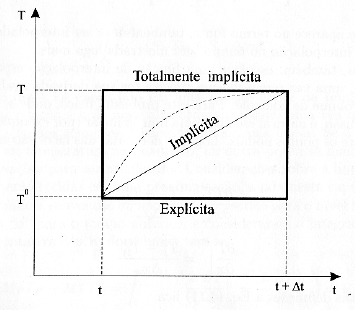
\includegraphics[width=8cm]{Imagenes/Funcion_Interpolacion.png}
% \caption[Función de interpolación en el tiempo]{Función de interpolación en el tiempo. Modificado de Maliska(2006) \cite{Maliska2017TransferenciaEd..}}
% \label{fig:fig34}
% \end{figure}
% %/////////////////////////////////////////////////////////////////////////////////////////


% %........................................................................................
% % TITULO DE LA SUBSECCIÓN 3.4.2.4
% \subsubsection{Medio Poroso Saturado}~\hypertarget{sec:sec3424}{}
% \label{sec:sec3424}




% %........................................................................................
% % TITULO DE LA SUBSECCIÓN 3.4.2.5
% \subsubsection{Medio Poroso Parcialmente Saturado}~\hypertarget{sec:sec3425}{}
% \label{sec:sec34245}





















% %----------------------------------------------------------------------------------------
% % TITULO DE LA SECCIÓN 3.5
% \section{Modelo Computacional}~\hypertarget{sec:sec350}{}
% \label{sec:sec350}


% %........................................................................................
% % TITULO DE LA SUBSECCIÓN 3.5.1
% \subsection{Consolidación Unidimensional}~\hypertarget{sec:sec351}{}
% \label{sec:sec351}

% %........................................................................................
% % TITULO DE LA SUBSECCIÓN 3.5.1.1
% \subsubsection{Realidad}~\hypertarget{sec:sec3511}{}
% \label{sec:sec3511}


% %........................................................................................
% % TITULO DE LA SUBSECCIÓN 3.5.1.2
% \subsubsection{Modelo Conceptual}~\hypertarget{sec:sec3512}{}
% \label{sec:sec3512}


% %........................................................................................
% % TITULO DE LA SUBSECCIÓN 3.5.1.3
% \subsubsection{Modelo Numérico}~\hypertarget{sec:sec3513}{}
% \label{sec:sec3513}


% %........................................................................................
% % TITULO DE LA SUBSECCIÓN 3.5.1.4
% \subsubsection{Modelo Computacional}~\hypertarget{sec:sec3514}{}
% \label{sec:sec3514}


% %........................................................................................
% % TITULO DE LA SUBSECCIÓN 3.5.1.5
% \subsubsection{Resultados de la Simulación}~\hypertarget{sec:sec3515}{}
% \label{sec:sec3515}



% %........................................................................................
% % TITULO DE LA SUBSECCIÓN 3.5.1.6
% \subsubsection{Validación}~\hypertarget{sec:sec3516}{}
% \label{sec:sec3516}


% %........................................................................................
% % TITULO DE LA SUBSECCIÓN 3.5.2
% \subsection{Consolidación Bidimensional}~\hypertarget{sec:sec352}{}
% \label{sec:sec352}


% %........................................................................................
% % TITULO DE LA SUBSECCIÓN 3.5.2.1
% \subsubsection{Realidad}~\hypertarget{sec:sec3521}{}
% \label{sec:sec3521}


% %........................................................................................
% % TITULO DE LA SUBSECCIÓN 3.5.2.2
% \subsubsection{Modelo Conceptual}~\hypertarget{sec:sec3522}{}
% \label{sec:sec3522}



% %........................................................................................
% % TITULO DE LA SUBSECCIÓN 3.5.2.3
% \subsubsection{Modelo Numérico}~\hypertarget{sec:sec3523}{}
% \label{sec:sec3523}


% %........................................................................................
% % TITULO DE LA SUBSECCIÓN 3.5.1.4
% \subsubsection{Modelo Computacional}~\hypertarget{sec:sec3524}{}
% \label{sec:sec3524}


% %........................................................................................
% % TITULO DE LA SUBSECCION 3.5.1.5
% \subsubsection{Resultados de la Simulación}~\hypertarget{sec:sec3525}{}
% \label{sec:sec3525}


% %........................................................................................
% % TITULO DE LA SUBSECCIÓN 3.5.1.6
% \subsubsection{Validación}~\hypertarget{sec:sec3526}{}
% \label{sec:sec3526}



% %........................................................................................
% % TITULO DE LA SUBSECCIÓN 3.5.3
% \subsection{Problema \textit{Five-Spot}}~\hypertarget{sec:sec353}{}
% \label{sec:sec353}


% %........................................................................................
% % TITULO DE LA SUBSECCIÓN 3.5.4
% \subsection{Verificación del Modelo Numérico}~\hypertarget{sec:sec354}{}
% \label{sec:sec354}

